\documentclass[12pt,twoside,english]{book}
\usepackage{lmodern}
\renewcommand{\familydefault}{\rmdefault}
\usepackage[T1]{fontenc}
%\usepackage[latin9]{inputenc}
\usepackage[utf8]{inputenc}
\usepackage[a4paper]{geometry}
\geometry{verbose,tmargin=3cm,bmargin=3cm,lmargin=2cm,rmargin=2cm}
\setcounter{secnumdepth}{2}
\setcounter{tocdepth}{2}
\setlength{\parskip}{\smallskipamount}
\setlength{\parindent}{0pt}
\usepackage[para]{threeparttable}
\usepackage{babel}
\usepackage{float}
\usepackage{epigraph}
\usepackage{textcomp}
\usepackage[version=3]{mhchem}
\usepackage{amsthm}
\usepackage{bm}
\usepackage{amsmath}
\usepackage{graphicx}
%\graphicspath{{./figures/}}
\usepackage{setspace}
\usepackage{amssymb}
\onehalfspacing
\usepackage[unicode=true, 
 bookmarks=true,bookmarksnumbered=false,bookmarksopen=false,
 breaklinks=false,pdfborder={0 0 1},backref=false,colorlinks=false]
 {hyperref}
\hypersetup{
 pdfauthor={Bernardo Kyotoku}}
\author{Bernardo de B. C. Kyotoku}
\title{Applications in Optical Coherence Tomography and Advances into a Photonic Integrated Device} 
%\makeatletter
\date{March 12th 2011}
%%%%%%%%%%%%%%%%%%%%%%%%%%%%%% LyX specific LaTeX commands.
\providecommand*{\perispomeni}{\char126}
\AtBeginDocument{\DeclareRobustCommand{\greektext}{%
 \fontencoding{LGR}\selectfont\def\encodingdefault{LGR}%
 \renewcommand{\~}{\perispomeni}%
}}
\DeclareRobustCommand{\textgreek}[1]{\leavevmode{\greektext #1}}
\DeclareFontEncoding{LGR}{}{}

% Because converters don't know tabularnewline
\providecommand{\tabularnewline}{\\}

%%%%%%%%%%%%%%%%%%%%%%%%%%%%%% Textclass specific LaTeX commands.
\numberwithin{equation}{section}
\numberwithin{figure}{section}

%%%%%%%%%%%%%%%%%%%%%%%%%%%%%% User specified LaTeX commands.
\usepackage{soul}
\usepackage{color}
\usepackage{graphics}
\usepackage{hyperref}
\usepackage{array}
\usepackage[toc,sanitize={description=false}]{glossaries}
\newcommand\fnurl[2]{%
 \href{#2}{#1}\footnote{\url{#2}}%
}
\usepackage[natbib=true,bibstyle=numeric,citestyle=authortitle-icomp,firstinits,doi=false,url=false,isbn=false,labelyear=true]{biblatex}  
\bibliography{clean-abibliography}   
%\defbibheading{bibempty}{} 
\makeatother
\pagenumbering{roman}
\newacronym{FWHM}{FWHM}{full width half maximum}
\newacronym{GVD}{GVD}{group velocity dispersion}
\newacronym{FDL}{FDL}{Fourier delay line}
\newacronym{PSD}{PSD}{power spectrum density}
\newacronym{OCT}{OCT}{optical coherence tomography}
\newacronym{FDOCT}{FDOCT}{Fourier domain optical coherence tomography}
\newacronym{TDOCT}{TDOCT}{time domain optical coherence tomography}
\newacronym{SSOCT}{SSOCT}{swept source optical coherence tomography}
\newacronym{FFT}{FFT}{fast Fourier transform}
\newacronym{SROCT}{SROCT}{spectral radar optical coherence tomography}
\newglossaryentry{slab waveguide}{name=slab waveguide,description=}
\newacronym{FSR}{FSR}{free spectral range}
\newacronym{TE}{TE}{transversal electric}
\newacronym{TM}{TM}{transversal magnetic}
\newacronym{WDM}{WDM}{wavelength division multiplexer}
\newacronym{FRC}{FRC}{fiber reinforced composite}
\newacronym{CBVT}{CBVT}{cone beam volumetric tomography}
\newacronym{SPM}{SPM}{self phase modulation}
\newacronym{RES}{RES}{ring enhanced spectrometer}
\newacronym{PIC}{PIC}{photonic integrated circuit}

\newglossaryentry{coherence length}{name=coherence length,description=}

\makeglossaries
%\def\glstoc
\begin{document}
\maketitle
\chapter*{Abstract}
Optical coherence tomography is a non-invasive imaging technique that uses non-ionizing infrared radiation to probe few millimeter depth of target at resolution of few micrometers. Here we expose the theoretical basis to understand the technique. The text covers the two varieties of OCT --- time domain and frequency domain--- and discribe three applications of this technique to dentistry: a) One in the evaluation of crack propagation in fiber reinforced polymers used for dental restoration; b) The imaging of remains dentin and pulp chamber after dentin excavation for the purpose of measurement of dentin thickness, and c) a clinical evaluation of the integrity of dental restoration. In all these applications, OCT has outstanding imaging results and provides semiquatitative insight into the dental structure.

With the aim of developing optical coherence tomography integrated to a chip, we expose the theoretical basis of integrated photonics platform. After literature review, we detected that no integrated spectrometer, and OCT component, with the needed specifications exists. We, then, developed a spectrometer with the necessary features. This was possible due the creation of novel spectrometer architecture based on the combination of a ring resonator and a diffraction grating spectrometer.

\chapter*{Resumo}
Tomografia por coerência óptica (OCT) é uma técnica de imageamento não invasiva que usa radiação infravermelho para sondar alguns milímetros the profundidade de um alvo com um resolução de poucos micrômetros. Aqui, nós expomos a base teórica para entender a técnica. O texto cobre as duas variedades de OCT --- domínio temporal e domínio da frequência --- e descreve três aplicações da técnica em odontologia: a) Um na avalição the propagação rachaduras em polímeros reforçado com fibra usado em restauração dental; b) O imageamento da sobra de dentina e cavidade pulpar após excavação da dentina, com o propósito de medir a espessura da dentina, e c) uma avaliação clínica da integridade de restaurações dentais. Em todas essa aplicações, OCT gerou imagens marcantes e forneceu informações semiquatitativas sobre a estrura dentária.

Com o objetivo de desenvolver um sistema de tomografia óptica integrada em um chip. Nós expomos a base teórica da plataforma de fotônica integrada. Após uma revisão literária, nós descobrimos que não existe espectrômetro integrado com a especificações necessárias para uso em OCT. Nós, então, desenvolvemos um espectrômetro com a características necessárias. Isso foi possível devido a uma nova arquitetura de espectrômetro baseada na combinação de um ressoador em anel e um espectrômetro de grade de difração.

\tableofcontents{}

\phantomsection
\chapter*{Introduction}
\pagenumbering{arabic}
\addcontentsline{toc}{chapter}{Introduction}
\thispagestyle{myheadings}\markboth{INTRODUCTION}{}
%\epigraph{People are like resonators, drive them in the wrong frequency and they are not going to resonate. If you want them to work in a different rhythm, changing solely the driving frequency won't do the job. You have to change the underlying structure that defines each person natural beat.}{Bernardo Kyotoku}

In the middle of 2005, I started working in Prof. Anderson Gomes research group. At the time, my first assignment was to make improvements to the \gls{OCT} system available, a \gls{TDOCT} system. The delay line was composed by a mirror that was scanned using a DC motor. Each scan would take about half a minute to complete. A whole image needed 2 hours to be acquired. During the acquisition time, the lab needed to be in silence. And the final image could only be seen after the whole acquisition was done. Because of the acquisition time, in vivo imaging was out of question. It used a table top femtosecond laser as the light source, and therefore, it could not be moved unless you take the whole laser with you. The system would misalign frequently, therefore a long trying period was needed to operate the system. Fast forward to today, we built a \gls{SROCT} which can aquire an image in few seconds. Clinical trials have been performed. The system can be transported anywhere in a car by a single person. 

In 2008 we started an effort to integrate the whole \gls{OCT} system into a single chip. For this we started a cooperation with prof. Michal Lipson from Cornell University. She was leading her research group to develop photonics integrated in silicon chips component and systems. I was suppose to leverage the group technical knowledge to build the desired device. We quickly learned that no integrated spectrometer with the specifications needed to compose a OCT has ever been made. So we set to design such component. After two years we were able to achieve an integrated spectrometer with unprecedent resolution and compactness.

This thesis is divided in two parts. The first part, comprised of the first three chapters, concerns only optical coherence tomography. There are two modalities of OCT, time or frequency domain. And a review of each modality is given in the first two chapters. In its respective chapter, the implementations of each modality is described. In the third chapter we present three applications where these OCT systems were used. In the first application we use OCT to evaluate crack evolution in fiber reinforced polymers after mechanical cycling. The main used of this material is as a teeth prosthetic. We showed the possibility of OCT to non destructively evaluate of the prosthetic integrity. In the second application we report the generation of images of the remaining dentin and pulp chamber of in vitro human teeth. Last, in the third chapter we report a clinical assessment of dental restoration in humans, where lesions and failed restorations were succesfully identified where conventional visual and X-ray examination failed. 
\thispagestyle{myheadings}\markright{INTRODUCTION}

The second part of the thesis deals with subject needed in the design of spectrometers integrated on silicon chips. Fourth chapter provides a review on chip photonics circuit, laying the theoretical basis used throughout the remaining of the thesis. In the fifth chapter, the basics of free space and integrated spectrometers is given, and a first implementation of an integrated device is described. In the sixth chapter we describe the principle and details of the implementation of a technique that greatly improves the resolution and compactness of the integrated spectrometer.

%\part{Optical Coherence Tomography}
\chapter[Time Domain OCT]{Time Domain Optical Coherence Tomography}
\label{chapter:TDOCT}
\epigraph{I can only show you the door. You have to walk through it.}{Morpheus}

Superman's ability to see through walls always fascinated us. We have walked great lengths to achieve the same ability. Rottingen X-rays, ultrasound, nuclear magnetic resonance, computed tomography are some of the attempts to do this. Unfortunately any technique has a limited operational range which it works. X-rays cannot distinguish small density contrast, and is highly carcinogenic. Ultrasound does not achieve the same resolution possible by X-rays, nor can it achieve high velocity contrast. Although, in principle the problem could be circunvented, nuclear magnetic resonance does not work on non hydrogenated targets. Furthermore, its high maintenance cost restricts its use to high value applications. Here we discuss another prospective method, called optical coherence tomography. This technique is based on infrared interferometric measurements. It features, resolution on the order of its probing wavelength, real-time video imaging capability. The observable depth is limited by the absorption and scattering of the material being probed, which is typically a few millimeters for biological samples.

\section{Theory}

In OCT, the kind of interferometry used is the low-coherence type. In this section, we describe how low-coherence interferometry is used to measure the distance of an object with more than one reflecting surface.

\subsection{Michelson interferometer}
\label{sub:Michelson interferometer}
%
\begin{figure}[h]
\center{\input{interferometer.pdf_tex}}
\caption{Michelson interferometer\label{fig:Michelson-interferometer}}
\end{figure}
Consider the interferometer shown in figure \ref{fig:Michelson-interferometer}. To simplify the analysis, ignore the light polarization and dispersion effects. A light source emits a radiation, whose electric field is described by $E_{\text{in}}\left(t\right)$, upon a beam splitter. This light is divided and a fraction $D$ of its power is directed to mirror $S$ with reflectivity $R_{s}$. The light is reflected and returns to the beam splitter, where a fraction $\left(1-D\right)$ of its power goes to the detector. Similarly, in the other interferometer arm, $\left(1-D\right)$ of the light emitted by the light source is redirected to the mirror $R_{r}$, which is reflected and returns to the beam splitter, where a fraction $D$ of this light is redirected back to the detector. The electric field at the detector can be described by
\begin{equation}
E_{\text{out}}=\sqrt{K_{0}}E_{\text{in}}\left(t-\tau_{s}\right)-\sqrt{K_{r}}E_{\text{in}}\left(t-\tau_{r}\right),\label{eq:Simplest Field equation}
\end{equation}
where $K_{i}=R_{i}D\left(1-D\right)$ is the light power fraction that is shined to the detector and $\tau_{i}$ is the time the light takes to go from the beam splitter to the mirror $i$ and back.

The relationship between the output light intensity $\left\langle I\right\rangle $ and the mean electric field is:
\begin{equation}
\left\langle I\right\rangle =\left\langle \frac{\left|E\left(t\right)\right|^{2}}{2\eta_{0}}\right\rangle ,\label{eq:intensity field relation}
\end{equation}
where $\eta_{0}=\sqrt{\frac{\mu_{0}}{\varepsilon_{0}}}$ is the free space impedance. Using \ref{eq:Simplest Field equation} and \ref{eq:intensity field relation}, we get the intensity at the detector 
\begin{equation}
\left\langle I\right\rangle =\left\langle I_{\text{DC}}\right\rangle +\sqrt{K_{s}K_{r}}\Re\left(\Gamma\left(\tau_{s,r}\right)\right)\label{eq:michelson output intensity equation}
\end{equation}
where $\tau_{r,s}=\tau_{s}-\tau_{r}$ and $\Re\left(x\right)$ is the real part of $x$. We define the autocorrelation function for the electric field as
\begin{equation}
\Gamma\left(\tau\right)=\frac{E\left(t-\tau\right)E^{*}\left(t\right)}{\eta_{0}}
\label{eq:autocorrelation definition}
\end{equation}
and
\begin{equation}
\left\langle I_{\text{DC}}\right\rangle =\sum_{j}K_{j}\left\langle I_{0}\right\rangle ,
\end{equation}
where $\left\langle I_{0}\right\rangle =\left\langle \frac{\left|E_{0}\left(t\right)\right|^{2}}{2\eta_{0}}\right\rangle $ is the mean light intensity that leaves the source, which in this case is constant. More specifically, it is of interest that the light source should be stationary in the wide sense, which means
\begin{enumerate}
\item $\left\langle E\left(t\right)\right\rangle $ is independent of $t$.
\item $\left\langle E\left(t_{1}\right)E^{*}\left(t_{2}\right)\right\rangle $
depends only on the difference $\tau=t_{2}-t_{1}$, not the absolute values of $t_1$ and $t_2$.
\end{enumerate}

\subsection{Optical interferometry with coherent light}

%
\begin{figure}[h]
\input{interferometerGraphics.pdf_tex}\caption{Light intensity at the interferometer output for input source of (a)
coherent light. (b) light with coherence length $\Delta l_{c}$.\label{fig:interferometerGraphics}}

\end{figure}


If the light is perfectly coherent (i.e. monochromatic), then its electric field can be described as $E_{\text{in}}\left(t\right)=E_{0}e^{-i2\pi\nu t}$ where $\nu$ is the optical frequency and $E_{0}$ is the field amplitude. Replacing $E_{\text{in}}\left(t\right)=E_{0}e^{-i2\pi\nu t}$ in equation \ref{eq:autocorrelation definition} and using \ref{eq:michelson output intensity equation}, we get
\begin{equation}
\left\langle I\right\rangle =\left\langle I_{\text{DC}}\right\rangle +2\left\langle I_{0}\right\rangle \sqrt{K_{s}K_{r}}\cos\left(2\pi\nu\tau_{s,r}\right),\label{eq:interference coherent delay}\end{equation}
or, using $\lambda=c/\nu$ and $\Delta l=\frac{c}{2}\left(\tau_{s}-\tau_{r}\right)$
\begin{equation}
\left\langle I\right\rangle =\left\langle I_{\text{DC}}\right\rangle +2\left\langle I_{0}\right\rangle \sqrt{K_{s}K_{r}}\cos\left(2\pi\frac{\Delta l}{\lambda/2}\right).\label{eq:interference coherent length}\end{equation}
Equation \ref{eq:interference coherent length} says that the light intensity in the detector varies periodically with the interferometer arm length difference $\Delta l$, with period $\lambda/2$. In special, in the case where $K_{s}=K_{r}$ we get points of zero intensity, as illustrated in \ref{fig:interferometerGraphics}(a). 


\subsection{Low-coherence interferometry}
\label{sub:Low-coherence interferometry}

In practice, the longitudional coherence of a light source is always limited. In a real case, overlapped with the rapid intensity oscillation with period $\lambda/2$, we will notice a gradual decrease of oscillation amplitude. The full width a half maximum of the oscillation envelope is called \gls{coherence length} $\Delta l_{c}$, which we are going to show to be inversely proportional to the light source bandwidth.

Consider the interferometer in figure \ref{fig:Michelson-interferometer}, now illuminated with a low coherence light, whose spectrum lineshape is described by $G\left(\nu\right)$. The mean light intensity at the detector can be described by the equation \ref{eq:michelson output intensity equation}. According with the \fnurl{Wiener-Khinchin theorem}{http://en.wikipedia.org/wiki/Wiener-Khinchin_theorem}\footcite{Goodman:1985p2703}, the autocorrelation of the signal and its \gls{PSD} are related by a Fourier transform
\begin{equation}
G\left(\nu\right)=\int_{-\infty}^{\infty}\Gamma\left(\tau\right)e^{i2\pi\nu\tau}d\tau\label{eq:spectrum from autocorrelation}\end{equation}
\begin{equation}
\Gamma\left(\tau\right)=\int_{-\infty}^{\infty}G\left(\nu\right)e^{-i2\pi\nu\tau}d\nu\label{eq:autocorrelation from spectrum}\end{equation}
If the light source \gls{PSD} lineshape is Gaussian
\begin{equation} G\left(\nu\right)=\frac{\left\langle I_{0}\right\rangle }{\Delta\nu}\sqrt{\frac{4\ln2}{\pi}}e^{-4\ln2\left(\frac{\nu-\nu_{0}}{\Delta\nu}\right)^{2}},\label{eq:gaussian spectrum}\end{equation}
where $\nu_{0}$ is the central optical frequency, $\Delta\nu$ is the \gls{FWHM} of the Gaussian. The autocorrelation of this spectrum is
\begin{equation}
\Gamma\left(\tau\right)=\left\langle I_{0}\right\rangle e^{-i2\pi\nu_{0}\tau}e^{-\ln2\tau^{2}/\Delta\tau_{c}^{2}}\label{eq:gaussian autocorrelation function}\end{equation}
where $\Delta\tau_{c}=\frac{2\ln2}{\pi\Delta\nu}$ is called the \emph{coherence time}, or alternatively using $\tau=\frac{2\Delta l}{c}$
\begin{equation}
\Gamma\left(\Delta l\right)=\left\langle I_{0}\right\rangle e^{-i2\pi\frac{\Delta l}{\lambda_{0}/2}}e^{-\ln2\frac{\Delta l^{2}}{\left(\Delta l_{c}/2\right)^{2}}}\label{eq:gaussian autocorrelation function by distance}\end{equation}
where $\Delta l_{c}=\frac{2\ln2c}{\pi\Delta\nu}=\frac{2\ln2\lambda_{0}^{2}}{\pi\Delta\lambda}$ is defined as \emph{coherence length}. $\lambda_{0}$ the central wavelength. Replacing \ref{eq:gaussian autocorrelation function by distance} on \ref{eq:michelson output intensity equation} we get
\begin{equation} \left\langle I\right\rangle =\left\langle I_{\text{SD}}\right\rangle +2\left\langle I_{0}\right\rangle \sqrt{K_{s}K_{r}}\cos\left(2\pi\frac{\Delta l}{\lambda_{0}/2}\right)e^{-i2\pi\frac{\Delta l}{\lambda_{0}/2}}e^{-\ln2\frac{\Delta l^{2}}{\left(\Delta l_{c}/2\right)^{2}}}\label{eq:gaussianInterferogram}\end{equation}
Equation \ref{eq:gaussianInterferogram} justifies the behavior of the light intensity at the interferometer output described in the beginning of section and illustrated in \ref{fig:interferometerGraphics} (b). The cosine is responsible for the rapid oscillation and the Gaussian modulates the oscillation amplitude, which falls to half at a distance $\Delta l_{c}/2$. As described earlier, the coherence length is inversely proportional to the light spectrum. The specific power spectrum lineshape of the source alters the autocorrelation function, but the fact that the coherence length decreases with the increase of the power spectrum width of the light source is not altered.

\subsection{Low coherence interferometry with multi-layer structures}

%
\begin{figure}[h]
\begin{minipage}[t]{0.48\columnwidth}%
\input{interferometerSample.pdf_tex}\caption{Interferometer with low coherence light source and micro-structured sample. \label{fig:interferometer_sample}}
%
\end{minipage}\hfill{}%
\begin{minipage}[t]{0.48\columnwidth}%
\input{interferogram-TD.pdf_tex}\caption{Intensity at detector as the reference arm is scanned.\label{fig:interferometer2}}
%
\end{minipage}
\end{figure}


To describe the reconstruction of the longitudional image of a structure, we replace the $s$ mirror by a sample with dielectric layers. The input beam is focused onto the sample surface, as shown in figure \ref{fig:interferometer_sample}. We can model the electric field at the interferometer output coming from the sample arm as
\begin{equation}
E_{s}\left(t\right)=\sum_{i}K_{i}E_{0}\left(t-\tau_{i}\right),
\end{equation}
where $E_{0}\left(t\right)$ is the light source field and $K_{i}=R_{i}\left(1-D\right)D$, $D$ being the beam splitter splitting ratio, $R_{i}$ is the reflectivity of the $i$-th sample interface and $\tau_{i}$ is the round-trip time from the beam splitter to the $i$-th sample interface. The intensity at the detector will then be
\begin{equation}
\left\langle I\right\rangle =\left\langle \frac{\left|E_{s}\left(t\right)+E_{r}\left(t\right)\right|^{2}}{2\eta_{0}}\right\rangle =\left\langle I\right\rangle +\sum_{i}\sqrt{K_{i}K_{r}}\Re\left[\Gamma\left(\tau_{r,i}\right)\right]\end{equation}
where $E_{r}\left(t\right)=K_{r}E\left(t-\tau_{r}\right)$ is the light electric field that comes from the reference mirror and $\tau_{r}=2\Delta l/c$. For a sample shown in figure \ref{fig:interferometer_sample}, the intensity as a function of the delay $\tau_{r}$, will be as shown in the black line in figure \ref{fig:interferometer2}, what we call \emph{interferogram}. In it, we can identify three packets, each corresponding to a light returning from each of the sample interfaces.
The interval time between packages is equal to the time light takes to go from one interface to the other and return, $\tau_{x}=n_{g}\Delta l_{x}/c$, where $n_{g}$ is the group index of the material that the light is propagating at.

An interferogram can be acquired by detecting the output light as the reference mirror is scanned, and this is denominated A-Scan. The detected electronic signal passes through an envelope detector circuit. This circuit eliminates the oscillation within the packets, leaving the envelope of the signal, as shown in red on the graph \ref{fig:interferometer2}, to which we call \emph{tomogram}. An image is made by translating the beam transversally to the beam direction and taking a tomogram after a chosen step size.


\subsection{Detector signal}

The mean current generated by the photo-diode can be described as
\begin{equation}
\left\langle i\right\rangle =\frac{e\eta}{\eta\nu_{0}}\left\langle P\right\rangle ,\end{equation}
where $\left\langle P\right\rangle =A\left\langle I\right\rangle $ is the mean light power that hits the detector in the area $A$, $\eta$ is the detector quantum efficiency, $e$ is the electron charge and $h$ is the Planck constant. If we scan the reference mirror at a velocity $u_{r}$ in the low coherence interferometer described previously, the current will be
\begin{equation}
\left\langle i\right\rangle =\frac{e\eta}{\eta\nu_{0}}\left[\left\langle P_{\text{DC}}\right\rangle +2\left\langle P_{0}\right\rangle \sqrt{K_{s}K_{r}}\cos\left(2\pi\nu_{r}t\right)e^{-i2\pi\frac{\Delta l}{\lambda_{0}/2}}e^{-\ln2\frac{u_{r}^{2}t^{2}}{\left(\Delta l_{c}/2\right)^{2}}}\right],\end{equation}
where $\nu_{r}=\frac{u_{r}}{\lambda_{0}/2}$. To remove some noise in the detector current, the signal is filtered using an electronic pass band filter centered at $\nu_{r}$ with bandwidth $B$,
\begin{equation}
B\approx\frac{u_{r}\Delta\nu}{c}\sqrt{\frac{\pi}{\ln2}}\end{equation}
which removes the DC current due to the term $\left\langle P_{DC}\right\rangle $. 

The electric peak current of the interference pattern at $\Delta l=0$ is
\begin{equation}
\left\langle i\right\rangle =\frac{2e\eta}{h\nu_{0}}\left\langle P_{0}\right\rangle \sqrt{K_{r}K_{s}}.\label{eq:current intensity relation}\end{equation}
Equation \ref{eq:current intensity relation} shows that the electric current is proportional to the square root of the light power fraction that returns form the sample $K_{s}$ and the reference mirror $K_{s}$, which shows a heterodyne amplification of the signal coming from the sample.


%\section{Reflectivity Sensitivity}
%
%In a OCT system it is of interest to know what is the smallest interface reflectivity that can be observed. The quantity is referenced as \emph{reflectivity sensitivity} or more simply \emph{sensitivity}.
%
%
%\subsection{Effective reflectivity vs interface reflectivity}
%
%
%\subsection{Signal to noise ratio}
%
%The signal to noise ratio (SNR) is a physical quantity of $i$ defined as
%\begin{equation}
%\text{SNR}=\frac{\left\langle i\right\rangle ^{2}}{\sigma_{i}},\end{equation}
%where $\left\langle i\right\rangle $ and $\sigma_{i}^{2}$ are, respectively, the mean and the variance of the current $i$. Physically, the definition tell how great is the information $\left\langle i\right\rangle $ compared to the mean fluctuations amplitude $\sigma_{i}$ due to noise. 
%
%
%\subsection{Noise sources}
%
%The noise shown here in the detection band used can be considered white noise with zero mean and non correlated. The outcome of that is that the variance of the noise signals sum is equal to the sum of the variance of each noise signal.
%\begin{equation} \sigma_{i}=\sum_{n}\sigma_{n}^{2}\end{equation}
%\subsubsection{Shot noise}
%
%Noise due to the quantizationvd of light and electric current. The quantity of photons arriving at the detector in a sampling interval $\Delta t$ is not constant, even if the power of the light source is. The distribution of the number of photons hitting the detector as a poissonian lineshape, whose width is equal to the mean number of photons. In addition to that, the photo-electron generation occurs with a probability $\eta$, defined as quantum efficiency. It can be shown, that the photo-electron current has a variance
%\begin{equation}
%\sigma_{s}^{2}=e\left\langle i\right\rangle B,\end{equation}
%where $e$ is the electron charge and $B$ is the detection bandwidth of the circuit.
%
%
%\subsubsection{Relative intensity noise}
%
%Relative intensity noise (RIN) are noise that grows linearly with the mean photo-current power. A few examples include the optical source power fluctuations. The noise spectral density can be model with a white noise over the band of interest. Therefore, the variance of this noise can be described as
%\begin{equation}
%\sigma_{RIN}^{2}=e\gamma\left\langle i\right\rangle ^{2}B,\end{equation}
%where the parameter $\gamma$ is experimentally measured. In practice it is possible to remove this noise using a balanced detection system. We therefore will not take this noise into consideration in the final calculation.
%
%
%\subsubsection{Thermal noise}
%
%There are two main forms of thermal noise. One during detection, when black body radiation and thermal phonons in the detector causes the excitation of electrons generating a current with mean $\left\langle i\right\rangle =e\beta k\theta$ and variance
%\begin{equation}
%\sigma_{\theta1}^{2}=e\beta k\theta B,\end{equation}
%where $\beta$ is a detector geometry and material constant, $\theta$ is the temperature and $k$ is the Boltzmann constant. Since its value is of the order of $3\times10^{-15}$ A in room temperature, we will not take it into account.
%
%Also called Johnson-Nyquist noise is the electronic noise generated by the thermal agitation of the charge carriers (usually the electrons) inside an electrical conductor at equilibrium, which happens regardless of any applied voltage. It is a zero mean noise with variance equal
%\begin{equation}
%\sigma_{\theta2}^{2}=4k\theta RB,\end{equation}
%where $R$ is the conductor resistance.
%
%
%\subsection{Sensitivity optimization}
%

\section{Fourier delay line TDOCT}
\begin{figure}
%\begin{minipage}[t]{0.48\textwidth}
\centering\input{fdl.pdf_tex}
\caption{Fourier delay line schematics.}
\label{fig:fdl}
%\end{minipage}
%\hfill
%\begin{minipage}[t]{0.48\textwidth}
%\end{minipage}
\end{figure}

One of the models of \gls{TDOCT} built used a Fourier delay line. This delay line allows a high A-scan frequency. The basic idea consists of adding, to the light beam, a linear phase delay in the frequency domain, which in the time domain correspond to a temporal delay. This effect is produced by resolving spatially the light wavelength and adding a different time delay to each different wavelength by using a lens and a mirror, as shown in figure \ref{fig:fdl}. The temporal delay to each optical frequency is\footcite{Rollins:1998p1700}
\begin{equation}
\phi\left(\theta\right)=\frac{8\pi\nu z_0\theta}{c}-\frac{8\pi f\left(\nu-\nu_0\right)\theta}{a\nu_0},
\label{eq:delay frequency}
\end{equation}
where $f$ is the lens focal length, $a$ is the grating pitch, $\theta$ is the angle between the mirror surface and the lens plan, $z_0$ is the distance between the mirror rotation axis and the trajectory of the beam central optical frequency $\nu_0$. The effect of replacing the standard delay line by a Fourier delay line can calculated as follows. Considering the incoming beam in the reference arm as $E\left(t\right)$, whose spectrum amplitude is $g\left(\nu\right)$. Returning from the delay line the returning beam spectrum amplitude will be
\begin{equation}
\tilde{g}\left(\nu\right)=g\left(\nu\right)e^{i\phi\left(\theta\right)},
\label{eq:fdl return spectrum amplitude}
\end{equation}
and the electric field will be $\tilde{E}\left(t\right)$. The power intensity of the beam coming from from both arms of the interferometer, as described at section \ref{sub:Michelson interferometer}, will be
\begin{eqnarray}
\left<I\right>&=&\frac{\left<\sqrt{K_{0}}E_{0}\left(t-\tau_{s}\right)+\sqrt{K_{r}}E_{0}\left(t-\tau_{r}\right)\right>}{2\eta_0}\\
&=&\left<I_{DC}\right>+\left<I_0\right>\sqrt{K_s K_r}\Re\left[{\Xi\left(\tau\right)}\right],
\label{eq:fdl interferometer output intensity}
\end{eqnarray}
where $\tau$ is the delay due to the path-length difference between the interferometer arms when $\phi=0$, and
\begin{equation}
\Xi\left(\tau\right)={\left<E\left(t\right)\tilde{E}^*\left(t-\tau\right)\right>}{\eta_0},
\end{equation}
is the cross correlation between $E\left(t\right)$ and $\tilde{E}\left(t\right)$. According to the cross correlation theorem
\begin{equation}
\Xi\left(\tau\right)=\int_{-\infty}^{\infty}\left\langle g\left(\nu\right)\tilde{g}^{*}\left(\nu\right)\right\rangle e^{-i2\pi\nu\tau}d\nu,
\label{eq:cross correlation theorem}
\end{equation}
knowing that $\left|g\left(\nu\right)\right|^{2}=G\left(\nu\right)$. Using \ref{eq:fdl return spectrum amplitude}, \ref{eq:delay frequency} and \ref{eq:fdl interferometer output intensity}
\begin{equation}
\left\langle I\right\rangle =\left\langle I_{\text{DC}}\right\rangle +\left\langle I\right\rangle \sqrt{K_{r}K_{s}}\cos\left[2\pi\nu_{0}\left(\tau+\frac{4}{c}z_{0}\theta\right)\right]\Gamma\left[\tau+4\left(\frac{z_{0}}{c}-\frac{f}{a\nu_{0}}\right)\theta\right]
\label{eq:fdl final output intensity}
\end{equation}
where $\Gamma\left(t\right)$ is the same as defined before. From the auto-correlation function argument, we observe that the group delay $\tau_g$ varies linearly with the mirror angle $theta$
\begin{equation}
\frac{d\tau_{g}}{d\theta}=4\left(\frac{z_{0}}{c}-\frac{f}{a\nu_{0}}\right),
\end{equation}
and the phase delay $\tau_f$ we can obtain from the cosine argument
\begin{equation}
\tau_f=\frac{4z_0}{c}\theta.
\label{eq:fase delay}
\end{equation}
Varying the group delay $\tau_g$, by changing $\theta$, we execute an axial scan, while the variation on the phase delay $\tau_f$ causes an oscillation of any constructive interference. The A-scan is described by
\begin{equation}
\Delta l_g=\tau_g\frac{c}{n_g}=\frac{4}{n_g}\left(z-\frac{f\lambda_0}{a}\right)\Delta\theta.
\label{eq:delay angle}
\end{equation}
During scan the carrier frequency is dependent on the phase delay scan and will be equal
\begin{equation}
\nu_f=\frac{8\pi\nu_0 z_0}{c}\frac{d\theta\left(t\right)}{dt},
\label{eq:carrier frequency}
\end{equation}
which is of interest when choosing the frequency at which the signal will be filtered, the signal bandwidth will be
\begin{equation}
B=2\Delta\nu\sqrt{\frac{\pi}{\ln2}}\left(\frac{z_0}{c}-\frac{f}{a\nu_0}\right)\frac{d\theta\left(t\right)}{dt}.
\label{eq:signal bandwidth}
\end{equation}

\section{Implementation}

\begin{figure}
\begin{minipage}[t]{0.48\textwidth}
\input{FDL-whole-setup.pdf_tex}
\caption{OCT setup with Fourier delay line.}
\label{fig:OCTfdl}
\end{minipage}
\hfill
\begin{minipage}[t]{0.48\textwidth}
\input{FDL-setup.pdf_tex}
\caption{Fourier delay line setup.}
\label{fig:FDL setup}
\end{minipage}
\end{figure}


Figure \ref{fig:OCTfdl} shows the schematic of the time domain OCT system operating at the central wavelength of 1280 nm, maximum average power 5 mW, delivered by a superluminescent diode model no. SLD-571, SUPERLUM, Moscow, Russia, with a 64.6-nm bandwidth, which represents an axial resolution of 11 \textgreek{m}m. As with the system in figure \ref{fig:interferometer_sample}, we have a Michelson interferometer, but in this case the delay line is a Fourier domain delay line\footnote{Cense:2004p2285}, shown in detail in figure \ref{fig:FDL setup}. The recombined beams are fed into a photodetector and the signal is sent to a band-pass filter, a transimpedance amplifier and finally to a computer digitalizer, NI PCI-5122. The galvo motor signal is produced by a signal generator Agilent. The signal generator trigger signal is also sent to the PC digitalizer. The sample arm is carried by a 1-D linear translation stage powered by a computer controlled servo DC motor (Z625B, Thorlabs), and is responsible for beam transversal scan. The galvo scan rate was 100 Hz, while the transversal scanning speed was 1 mm/s. Envelope detection was performed computationally using a band pass filter.

\section{Fourier delay line alignment}

Refering to figure \ref{fig:FDL setup} a fiber optic coupler facilitated the system alignment since the alignment of the delay line could be uncoupled from the other arms. The first thing that needs to be done is to properly align the \gls{FDL} making sure that the first order diffraction central wavelength is orthogonal to the grating. This can be done by exploring the fact that the second order diffraction of the central wavelength must return to the input. Monitoring the return light using a fiber optic coupler connected to a spectrometer, the grating angle can be adjusted until the returning wavelength is the central wavelength. The galvo mirror can then be mounted and aligned such that the diffracted light central wavelength after reflection on the galvo mirror couples back to the fiber optics. Lens can then be placed and adjusted in the direction transversal to the beam until the the beam couples back to the fiber. Galvo mirror and lens should be roughly placed on the axial position. Fiber optic coupler should then be translated vertically by a few millimeters and the mirror M can be placed and aligned such that the returning beam couples back to fiber. FDL is roughly aligned to be placed in the interferometer. With a test sample, a polished surface, placed at half the FDL path-length distance from the sample fiber optic coupler. Setup the OCT interferometer with the output detector and a test sample and find an interference on a oscilloscope. Lens and galvo mirror axial rough adjustment will cause severe \gls{GVD} therefore do not expect clear interference signal. Couple the oscilloscope to AC and amplify the as much as the noise level clearly. After the interference is found, adjust the lens and galvo mirror axial position until the interference is as sharp as possible. The Fourier delay line is now adjusted.


\chapter[Fourier Domain OCT]{Fourier Domain Optical Coherence Tomography}
\label{chapter:FDOCT}
In 1995, Fercher et al.\footcite{Fercher:1995p1683} modified Wolf's solution of the optical inverse scattering problem to the one-dimensional problem of length measurement. The solution allowed the reconstruction of the scattering target structure through the Fourier transform of the backscattered light field for a bounded range of wavelengths. Due to the high frequency of light, it is not possible to directly measure its field. But using interferometric methods, one can back calculate the field, except for an ambiguity of $\pi$ in the field phase. This method is known as \gls{FDOCT}. By measuring the contribution of each wavelength separately a sensitivity higher than with \gls{TDOCT} can be achieved. This enabled the achievement of clinical 3D imaging with ultra-high resolution and in-vivo.

The first section of this chapter contains a rough picture of how \gls{FDOCT} works, followed by a more rigorous modeling and description of two variants of \gls{FDOCT}. A section on how to deal with the field phase $\pi$ ambiguity is also presented. The chapter is completed with details of one implementation of a \gls{FDOCT} system.

\section{Overview of Fourier domain OCT}

%
\begin{figure}[h]
	\centering\input{interferometer.pdf_tex}
	\caption{Michelson interferometer.}
	\label{fig:Michelson-interferometer-2}
\end{figure}


Before going through a more rigorous derivation, we will show a more intuitive picture on how frequency domain OCT reconstructs its image. Consider the Michelson interferometer illustrated on \ref{fig:Michelson-interferometer-2} and described in section \ref{sub:Michelson interferometer}. It was shown in section \ref{sub:Michelson interferometer} that the light intensity in the interferometer output is described by
\begin{equation} \left\langle I\right\rangle =\left\langle I_{0}\right\rangle +\frac{\sqrt{K_{r}K_{s}}}{\eta_{0}}\cos\left(2\pi\nu\tau_{r,s}\right).\end{equation}
Notice that the equation has a dual behavior relative to optical frequency $\nu$ and the time delay $\tau$. Usually, it is easier to vary the interferometer arm length keeping the optical frequency (or wavelength) constant and observe the light intensity at the interferometer output. We will then see interference fringes as graph on figure \ref{fig:freqGraphSimple}. But if we keep the arms length difference constant and equal $\Delta l=c\tau/2$, we can rewrite equation \ref{eq:interference coherent length} as
\begin{equation}
\left\langle I\right\rangle =\left\langle I_{0}\right\rangle +\frac{\sqrt{K_{r}K_{s}}}{\eta_{0}}\cos\left(2\pi\frac{2\Delta l}{c}\nu\right).\end{equation}
Notice that the oscillation period in inversely proportional to $\Delta l$. Therefore, if we know the period of the intensity oscillation in optical frequency $\Delta\nu$, we can calculate the difference of optical path-length between the interferometer arms, $\Delta l=\frac{c}{2\Delta\nu}$.

If we put dielectric sample in place of a sample mirror, as show in figure \ref{fig:InterferometerBiLayer}, instead of getting a simple intensity oscillation, we will obtain a superposition of several senoids described by the equation below
\begin{equation}
\left\langle I\right\rangle =\left\langle I_{0}\right\rangle \left[1+F_{r,1}\cos\left(2\pi\tau_{r,1}\nu\right)+F_{r,2}\cos\left(2\pi\tau_{r,2}\nu\right)+F_{1,2}\cos\left(2\pi\tau_{1,2}\nu\right)\right].\end{equation}
 
The second and the third terms in the brackets are related to the interference between the light from the reference mirror and the interfaces 1 and 2. The fourth term is due to the interference of the interfaces 1 and 2 between themselves. As can be seen in figure \ref{fig:graphics interference bi-layer}, it is difficult to identify the frequencies of each harmonic associated with the interference of light coming from two interfaces. However, we can identify the contribution of each harmonic by taking the Fourier transform of the power spectrum as illustrated in figure \ref{fig:ft graph interferometer bi-layer}.

The presence of the peaks due to the interference between the two interfaces of the sample are called \emph{self-interference}, and as can be seen, it creates reconstruction artifacts that obstruct the reconstructed image. However, note that the distance of the peak is equal to the sample thickness, and is independent of the distance between the interfaces and the reference distance. Therefore, if the distance of the sample surface to the reference is greater than the sample thickness $\Delta l_{1,r}>\Delta l_{1,2}$, all peaks after the position $\Delta l_{1,2}$ are free of the these artifacts. In the following section we will show other methods to suppress these artifacts.

%
\begin{figure}[h]
%
\begin{minipage}[t]{0.48\columnwidth}%
\input{freqInterferometerGraph.pdf_tex}\caption{Light intensity at the Michelson interferometer output as a function
of the source optical frequency. The interferometer arms length difference
can be calculated as $\Delta l=\frac{c}{2\Delta\nu}$.\label{fig:freqGraphSimple}}
%
\end{minipage}\hfill{}%
\begin{minipage}[t]{0.48\columnwidth}%
\input{BiLayerInterferometer.pdf_tex}\caption{Michelson interferometer with semi-transparent sample.\label{fig:InterferometerBiLayer}}
%
\end{minipage}
\end{figure}

In principle Fourier transform assumes the integration for infinite spectral range. In practice this is not possible, and this limitation causes the decrease of the precision with which the oscillation frequencies are estimated and therefore decreasing the resolution to which we can observe the interface.

In the shown example, the output spectrum in measured by varying the light source wavelength. This type of operation is called swept source. However, it is possible to use a light source with broad spectrum, and distinguish the contribution of each optical frequency using a spectrometer principle as in the spectral radar OCT.


\section{Frequency domain OCT}

Consider the interferometer depicted in \ref{fig:InterferometerBiLayer}. As explained in the \gls{TDOCT} chapter the electric field at the interferometer output can be modeled as
\begin{equation}
E\left(t\right)=\sqrt{K_{r}}E_{0}\left(t-\tau\right)+\sum_{i}\sqrt{K_{i}}E_{0}\left(t-\tau_{i}\right)\end{equation}
where $K_j$ is the fraction of the light power coming from the point $j$ and arriving at the interferometer output, and $\tau_j$ is the time the light take to go and return from the beam-splitter to the point $j$, where $j$ can be $r$ or $i$. The autocorrelation function of the output light electric field $\Gamma\left(\tau\right)=\left\langle E\left(t\right)E^{*}\left(t-\tau\right)\right\rangle $
\begin{equation}
\Gamma\left(\tau\right)=\left[K_{r}+\sum_{i}K_{i}\right]\Gamma_{0}\left(\tau\right)+\sum_{i}K_{r,i}\Gamma_{0}\left(\tau+\Delta\tau_{r,i}\right)+\sum_{i}K_{r,i}\Gamma_{0}\left(\tau-\Delta\tau_{r,i}\right)+\sum_{i\ne j}K_{i,j}\Gamma_{0}\left(\tau-\Delta\tau_{i,j}\right),\label{eq:FDautocorrelation}\end{equation}
where $K_{a,b}=\sqrt{K_{a}K_{b}}$, $\Delta\tau_{a,b}=\tau_{a}-\tau_{b}=\frac{2\Delta l_{a,b}}{c}$ and $\Gamma_{0}\left(\tau\right)=\left\langle E_{0}\left(t\right)E_{0}^{*}\left(t-\tau\right)\right\rangle $. And $a$ and $b$ can be either $r,i$ or $j$.

Before describing $\Gamma$, it is worth to recall that $\Gamma_{0}$ is a complex function and therefore so is $\Gamma$. However, we are interested on the $\left|\Gamma\right|$. In section \ref{sub:Low-coherence interferometry} we discussed the types of $\left|\Gamma_{0}\right|$ and how they are related to the light source power spectral density. For this section it is just worth remembering that it is a peak function centered at argument.

The first term of the equation \ref{eq:FDautocorrelation} will give rise to a peak centered at the origin, called the DC term. The second term is constituted of several peaks each centered at its respective delays $\Delta\tau_{r,i}$ and height proportional to its reflectance. This is the information which we are going to use in the image reconstruction.
The third them as repeated information of the second term but inverted relative to the origin, called \emph{mirror image}. The fourth term are self interferences, due to the interference of backscattered light in the sample only.

%
\begin{figure}[h]
%
\begin{minipage}[t]{0.48\columnwidth}%
\input{graphInterferenceBiLayer.pdf_tex}\caption{Light intensity at the Michelson interferometer with a semi-transparent sample as a function of the source optical frequency ($\left<I\right>$). \label{fig:graphics interference bi-layer}}
%
\end{minipage}\hfill{}%
\begin{minipage}[t]{0.48\columnwidth}%
\input{graphInterferenceBiLayerFT.pdf_tex}\caption{Fourier transform of $\left<I\right>$. Each peak is due to interference between the light coming from the combination of any two interfaces. \label{fig:ft graph interferometer bi-layer}}
%
\end{minipage}
\end{figure}

The principle of \gls{FDOCT} is based on calculating the autocorrelation function of the interferometer output light from its power spectrum density. According to the Wiener-Khinchin theorem the autocorrelation of a function and its power spectral density are related by a Fourier Transform. Therefore, the, power spectral density at the interferometer output is
\begin{equation}
G\left(\nu\right)=G_{0}\left(\nu\right)\left[\left(K_{r}+\sum_{i}K_{i}\right)+2\sum_{i}K_{r,i}\cos\left(2\pi\nu\Delta\tau_{r,i}\right)+2\sum_{i\ne j}K_{i,j}\cos\left(2\pi\nu\Delta\tau_{i,j}\right)\right],
\label{eq:FDOCT output spectrum}
\end{equation}
where $G_{0}$ is the light source \gls{PSD}. We see that the interferometer output \gls{PSD} is composed of interference fringes whose frequencies grows with the delays $\Delta\tau_{a,b}$, and is modulated by a envelope equal to the input light \gls{PSD}.

\section{Full range complex imaging reconstruction}
\label{section:quadrature}
The modulus of the autocorrelation of the interferometer output light can be calculated from the output \gls{PSD}. But as stated before we are only interested in the second term of the autocorrelation function.
\begin{equation} \left|\Gamma_{2}\right|=\sum_{i}K_{r,i}\left|\Gamma_{0}\left(\tau+\Delta\tau_{r,i}\right)\right|,\end{equation}
Several methods were developed to extract the this term from the autocorrelation function. Each method having it own virtues and shortcomings in terms of processing power, additional equipment, sensitivity to sample motion (relevant for in vivo imaging). Here we describe the method we used, which was the \emph{quadrature delayed spectrum}.

%Over the last few years, techniques to achieve full range complex imaging in \gls{FDOCT} have been suggested using a number of approaches. Phase-shifting methods were among the first attempts to achieve the full range imaging by directly measuring the complex components of the interference OCT axial scan (A scan) signals through shifting the phases of the reference beam in multiple steps.However, the complex conjugate rejection ratio is limited by the accuracy of the phase steps, including chromatic errors, in addition to the sample small movement and the mechanical stability of the interferometer, making the in vivo imaging difficult, if not impossible. Recently, with the polarization-based demodulation, the instantaneous acquisition of two phase shifted OCT signals was demonstrated to eliminate the depth degeneracy, which is, however, problematic for birefringence samples.
%
%The detection of the complex components of OCT signal using $3\times3$ optical	couplers	as	phase-shifting	elements allowed simultaneous detection of the real and imaginary parts of the interferogram. This requires two separate detectors for acquiring the quadrature components. Careful calibration and alignment in the spectrometers and wavelength-dependent splitting ratio in the coupler, however, limit its practical use. Another approach that used appropriate carrier frequency in the swept source OCT to separate the two mirror images has also been suggested to resolve the complex conjugate ambiguity. While plausible, it is currently not possible to implement this approach in the system that employs a broadband light source and a spectrometer for detection. 
%
%In SD-OCT depth resolved information is encoded in the cross spectral density function measured with a spectrometer located in the detection arm of an interferometer. A drawback of this method is that since the detected spectral density is a real function and therefore its Fourier transform is Hermitian, the reconstructed image is symmetrical about zero path difference. As a consequence one cannot distinguish between negative and positive optical path differences with respect to the reference mirror. These effects are of minor importance for measuring thin objects , because the reference arm can be shifted to a position where the mirror images do not affect the image of the measured object. However, if one wants to measure objects with larger depth extension where the whole measurement range is needed the mirror terms heavily decrease the image quality and make it difficult to interpret the collected data. Furthermore, the sensitivity decrease of SD-OCT with distance from the zero position makes a differentiation between positive and negative distances highly desirable because this would allow to place the object within the most sensible measurement range near the reference mirror position.
%
%A solution to this problem is to measure the phase of the spectral interferometric signal, thus providing access to the complex scattered field An inverse Fourier transform of the complex data directly provides the true object structure, eliminating any mirror terms. Various approaches to achieve full range complex SD-OCT were reported, essentially employing different variants of phase shifting interferometry. These methods require the recording of 2-5 A-scans at a given transversal sampling location, whereby the reference phase is shifted between the individual A-scans by piezo-driven reference mirrors or acousto-/electro-optic phase modulators. The disadvantages of these methods are that additional components are required and measurement speed is reduced by the requirement of multiple A-scans.
%
%The principle of \gls{FDOCT} is based on the inverse scattering theorem that states that the inverse Fourier transform of the spectral interference pattern yields the axial sample structure. Like in time domain OCT the axial resolution increases with larger optical bandwidth of the employed light source . However the achievable sensitivity of \gls{TDOCT} decreases in the shot noise limit with increasing spectral width of the light source, i.e. with increasing axial resolution. On the other hand \gls{FDOCT} sensitivity is independent of the spectral bandwidth . Hence it was possible for the first time to perform clinical 3D imaging with ultra-high resolution and in-vivo . Nevertheless the achievable maximum depth range scales with the resolution of the spectrometer. Larger optical bandwidth results in reduced spectrometer resolution and thus in smaller depth range. In principle one could use a detector with higher pixel number but this has severe implications on the optical design of the spectrometer to keep its diffraction limited performance. Also, the data volume to be dealt with increases with detector size and its handling becomes more challenging.

%\subsubsection{DC level removal}
%
%This method removes the DC peak of the reconstructed image. The basic principle relies on filtering out any component that does no change as the beam is transversally scanning the sample. This will include besides the DC term, also any back reflection in the fiber optics ends.
%
%\fnurl{Several numerical filtering}{http://en.wikipedia.org/wiki/Digital_filter}methods are available in ready to use software libraries in several programming languages, including C, LabView, Python, Matlab.

%\subsubsection{Image in clean area}
%
%balanced detection\footcite{Houser:1994p1780}
%\subsubsection{Auto-interference suppression double spectrum}
%
%\subsubsection{Differential Fourier domain method}
%
%\subsubsection{Heterodyne complex FDOCT}
%
%\footcite{Bachmann:2006p1691}


%\subsubsection{Quadrature Fourier domain method}

The method consists of acquiring the imaginary part of the two spectra, with the reference arm $\lambda_0/8$ shorter than the other. According with equation \ref{eq:FDOCT output spectrum}, if we add a small temporal delay $\delta\tau$ by changing the reference arm length by $\delta L=c\delta\tau/2$ the output spectrum will be
\begin{equation}
G_\delta\left(\nu\right)=G_{0}\left(\nu\right)\left[\left(K_{r}+\sum_{i}K_{i}\right)+2\sum_{i}K_{r,i}\cos\left(2\pi\nu\Delta\tau_{r,i}+2\pi\nu\delta\tau\right)+2\sum_{i\ne j}K_{i,j}\cos\left(2\pi\nu\Delta\tau_{i,j}\right)\right],
\label{eq:FDOCT output spectrum delay}
\end{equation}
if 
\begin{equation}
2\pi\nu\delta\tau=-\frac{\pi}{2},
\label{eq:quadrature condition}
\end{equation} 
then the output spectrum can be approximated to
\begin{equation}
G_\delta\left(\nu\right)=G_{0}\left(\nu\right)\left[\left(K_{r}+\sum_{i}K_{i}\right)+2\sum_{i}K_{r,i}\cos\left(2\pi\nu\Delta\tau_{r,i}+2\pi\nu\delta\tau\right)+2\sum_{i\ne j}K_{i,j}\cos\left(2\pi\nu\Delta\tau_{i,j}\right)\right].
\label{eq:FDOCT output spectrum sin}
\end{equation}
With the above spectrum at hand it is possible to make the complex Fourier transform. Straight Fourier transform will conserve the DC level and the auto-correlation terms. These terms can be eliminated by subtracting a spectrum from another, leaving us with
\begin{equation}
\Gamma=\left|FT\left[G+iG_{\delta}\right]-FT\left[G_{\delta}+iG\right]\right|+\left|FT\left[G+iG_{\delta}\right]\right|-\left|FT\left[G_{\delta}+iG\right]\right|.
\label{eq:quadrature equation}
\end{equation}
The above equation proposed by Gotzinger\footcite{Gotzinger:2005p1712} is one used by us to obtain the tomograms in FDOCT setups.

For the condition \ref{eq:quadrature condition}, a delay varying linearly with optical frequency needs to be performed. Although there are ways to do it, we preferred to rely on the fact that optical frequency does not change much over the spectrum, and approximate \ref{eq:quadrature condition} by $2\pi\nu_0\delta\tau=-\frac{\pi}{2}$. Due to this approximation there is a polychromatic phase error\footcite{Leitgeb:2003p1779} which we neglected in our device.



\section{First spectral radar implementation}
\label{section:Spectral radar implementation}

Two \gls{SROCT} setups were built. The first version was built only with components available in the laboratory, while the required parts were acquired to implement the new design.  
%A closer look at the peak, figure 3c shows the system experimental resolution of 6 \textpm{} 0.5 \textgreek{m}m, quite close to the theoretically calculated value of 5.6 \textgreek{m}m. With 2 mW of optical power incident on the sample, a system sensibility of 98 \textpm{} 5 dB was measured independently, following the procedure of Ref. \footcite{Leitgeb:2003p1678}. The figure is within the estimated value of 95 dB. The high sensibility error is attributed manly due to the light source instability. The data acquisition and image generation were controlled by a LabView supported software. The software acquired two sets of spectra, each with a different displacement in the reference arm. The acquisition was done while the sample was transversally moved after a couple of spectra were measured. Using spline interpolation, a spectra with points evenly distributed in frequency was obtained from a spectra that was evenly distributed in wavelength. Then, from each couple of spectra a tomogram was calculated using Eq. (3). During the scan all tomograms are laterally stacked forming a 2D matrix. By mapping a color (or gray intensity) to each value of the 2D matrix an image of the scanned sample is reconstructed.


\begin{figure}[h]
\small
\input{SROCT1.pdf_tex}
\caption{First spectral radar setup.}
\label{fig:SROCT setup 1}
\end{figure}

Figure \ref{fig:SROCT setup 1} shows the setup schematics of the first version of \gls{SROCT}. A titanium:sapphire mode-locked optical oscillator, operating at 800 nm with a spectral width of 10 nm and emitting pulses of 150 fs, was used as the initial system light source. The laser beam was coupled into 2.2 m of a monomode fiber (FS-SN-4224, Thorlabs), leading to a spectral broadening, due to dispersive self-phase modulation\footcite{Hsu:2002p2439}. The initial 10 nm spectral width and 500 mW of power was broadened to 50 nm. Apart from fiber optics for spectral broadening, the setup was built in free space. On the reference arm, the beam passes through a variable attenuator (VA1), a piece of glass for dispersion compensation, and is reflected on a mirror fixed to a piezo buzzer as a translator. In the probe arm, the beam passes through an achromatic lens which focuses the beam onto the sample which is supported by a computer controlled XYZ translation stage. The combined light from the sample and reference arms are then focused to a spectrometer (USB2000, OceanOptics), which measures the light spectrum and sends it to a PC through USB port.

An axial resolution of 6 \textgreek{m}m was achieved where the theoretical value was 5.6\textgreek{m}m. With 2 mW of optical power incident on the sample, a system sensibility of 98\textpm5 dB was measured, following the procedure by Leitgeb\footcite{Leitgeb:2003p1678}. The data acquisition and image generation were controlled by a LabView supported software. The quadrature delayed spectrum\ref{section:quadrature} technique was used to eliminate mirror image and DC components, where a piezo was used to add the quadrature phase shift. 

This setup was used in the study of crack propagation in fiber reinforced polymers accounted in section \ref{section:Fiber reinforeced composite analyses}.

%\begin{figure}[h]
%\center{\input{spectraloct.pdf_tex}}
%\caption{typical Michelson type spectral radar OCT setup.}
%\end{figure}e
\section{Second spectral radar implementation}
\begin{figure}[h]
\small
\begin{minipage}[t]{0.48\textwidth}
\input{SROCT.pdf_tex}
\caption{Spectral radar setup.}
\label{fig:SROCT setup 2}
\end{minipage}
\hfill
\begin{minipage}[t]{0.48\textwidth}
\input{spectrometer.pdf_tex}
\caption{Spectrometer schematics.}
\label{fig:spectrometer}
\end{minipage}
\end{figure}
The schematic setup of the second version of SROCT is shown in figure \ref{fig:SROCT setup 2}.  The broadband source is a superluminescent diode Broadband SLD Light source (S840, SUPERLUM) with central wavelength 850 nm and delivering up to 25 mW and with a 49.9-nm bandwidth, which gives an axial resolution of 6 \textgreek{m}m. After traveling through the all-fiber beam splitter, the reflected beams from the sample and mirror are recombined and sent through a purpose-designed spectrometer, subsection \ref{sub:spectrometer}. The maximum incident power on the sample was 5 mW. The output is sent to a personal computer with a LabView-based imaging program. 

\subsection{Spectrometer}
\label{sub:spectrometer}
In FDOCT a spectrometer with high acquisition rate (tens of thousand spectrums/second) and high resolution (<100 pm) is necessary. Due to these restrictive features there was no such device commercially available, leading us to develop our own spectrometer, schematics in figure \ref{fig:spectrometer}. For high acquisition rate, a linear CCD camera (SM2-CL-2014, Atmel) was used. This camera features a line reading rate of 10k lines/s, with each line containing 2048 pixels with bit depth of 12 bits. The amount of data generated by such configuration is 60 MB/s, which is not easily handled by most computer-device communication interfaces. This camera transferred data to the computer through a CameraLink interface. The diffraction grating used was a 1200 lines/mm volume phase holographic transmission grating (Wasatch Photonics), capable to diffract >0.6 of the incident light to the first order diffraction, enabling us to construct highly sensitive spectrometer. A resolution of 100 pm was achieved.
%\pagebreak
\subsection{Testing}

To test the setup, OCT images were obtained from slices of a tooth. Figures \ref{fig:SROCT2 test}(a), \ref{fig:SROCT2 test}(c), \ref{fig:SROCT2 test}(e) and \ref{fig:SROCT2 test}(g) represent OCT images of different samples restored in composite resin, and \ref{fig:SROCT2 test}(b), \ref{fig:SROCT2 test}(d), \ref{fig:SROCT2 test}(f) and \ref{fig:SROCT2 test}(h), their respective optical microscopy images. In figures \ref{fig:SROCT2 test}(a) and \ref{fig:SROCT2 test}(b) we can see an example of a well placed and sound restoration, whilst \ref{fig:SROCT2 test}(c)/\ref{fig:SROCT2 test}(d) and \ref{fig:SROCT2 test}(e)/\ref{fig:SROCT2 test}(f) show the presence of an air bubble (within the circle) close to the tooth restoration interface, as well as the dentin-enamel junction. The white appearance of the air bubbles in the optical microscopy images is due to the smear layer impregnation during the teeth sectioning with diamond wheel. Figures \ref{fig:SROCT2 test}(g) and \ref{fig:SROCT2 test}(h) show an aesthetic facet, in which it is possible to observe the tooth-restoration limits (arrows), the dentin-enamel junction and, specially, the use of different shades of composite resin (large rectangles).

%
\begin{figure}[]
\noindent \begin{centering}
\input{claudiafig3.pdf_tex}
\caption{Images of transversal section of teeth. (a),(c),(e) and (g) are OCT images. (b),(d),(f) and (h) are are micrographs of the respective OCT images}
\label{fig:SROCT2 test}
\par\end{centering}
\end{figure}

%\section{Swept source implementation\label{section:Swept source implementation}}
%
%this chapter details the design of a swept source optical coherence tomography system.
%\begin{figure}
%\centering{}\input{swept_source_setup_schematics.pdf_tex}\caption{}\label{fig:swept_source_setup_schematics}
%\end{figure}
%
%\subsection{light source}
%
%\footcite{huber:2006p1731}\fnurl{commercial swept source lasers}{http://www.thorlabs.com/newgrouppage9.cfm?objectgroup_id=1276}
%
%
%\subsection{detection and digitalization}
%
%\fnurl{common-path interferometer}{http://www.thorlabs.com/newgrouppage9.cfm?objectgroup_id=2955}
%
%\fnurl{NI PCI-5122}{http://sine.ni.com/nips/cds/view/p/lang/en/nid/13309}
%
%
%\section{signal processing}
%
%
%\subsection{Probe}
%
%\footcite{Sun:2010p837}\footcite{Yeow:2005p66}\footcite{Xie:2003p88}
%
%\section{Signal Processing}
%
%Volumetric and video rate optical coherence tomography generate large amount of data that needs to be processed before presented. Video rate imaging requires that the whole a whole image to be processed the frame rate, which is not a trivial task.
%
%Considering that the each line consists of $N_p$ points (typically in the range of 500 to 2000) and each image has $N_{l}$ lines (500 to 5000). Images are generated at a frame rate of $F$(Movies rate being 25Hz but as slow as 10 Hz are acceptable). The total number of points that needs to be processed per second $P$ is $P=N_{p}N_{l}F$. Which, using the numbers given before would be in the range $2.5\times10^{6}$ e $2.5\times10^{8}$ points per second.
%
%A concern is that part of the processing is a discreet Fourier transform which the fastest algorithm available (fast Fourier transform) is does the processing in order $O\mbox{\ensuremath{\left(n\log\mbox{n}\right)}}$, where $n$ is the number of points in the array the discreet Fourier transform is being performed at.

\chapter{Applications in Optical Coherence Tomography}

Several essays were made using the two OCT system previously described. Not being an exhaustive list we show here three applications made using those systems. The research effort were all published and were done mainly by Deborah Fonsêca\footcite{Fonseca:2009p1}, Cláudia Mota and Ana Karla Braz\footcite{Braz:2009p2143}. Most of the time the OCT systems were stable and easy to use, no direct assistance from my person was needed.

%A recent study evaluating the enamel-restoration interface using OCT, in which just one patient was reported, has been published and Negritu et al.\footcite{Negrutiu:2009p2189} used OCT and confocal microscopy to investigate dental structures and restoration materials using extracted teeth.

%Microleakage, either from small or microscopic openings between the margins of the composite restoration and tooth is considered to be a major cause of restoration failure\footcite{Xie:2008p2148}. Microleakage can also result in bacteria penetrating the tooth-restoration space and into dentinal tubules, where secondary decay may occur and bacterial toxins will irritate the pulp. The oral environment, including occlusal forces and temperature variation, as well as the differences between the physical properties of teeth and restorative materials, polymerization shrinkage, the coefficient of thermal expansion, and modulus of elasticity can all contribute to microleakage. According to previous literature, if poor bond strength exists between the tooth and restorative material, a failure of adhesion may be caused by polymerization shrinkage, and microscopic gaps at the tooth-restoration interface can subsequently form \footcite{DeMelo:2005p2100,Attar:2008p2147,Xie:2008p2148}.

%OCT has already been applied in vitro and in vivo to a variety of medical specialties, including Opthalmology\footcite{Huang:1991p1955} , Dermatology \footcite{Pierce:2004p1839}, Gastroenterology \footcite{Tearney:1996p2052}, Cardiology\footcite{Boppart:1997p1840} and Cellular Engineering \footcite{Yang:2006p2053}.
%
%The optical coherence tomography OCT consists of a new imaging technique for diagnosis that produces bi or three-dimensional pictures, with a few microns of spatial resolution, and has been widely used to study biotissues, as reviewed\footcite{Bouma:2002p2007}. This technique was initially used in ophthalmology\footcite{Huang:1991p1955}, where it is well developed and clinically used, but it has been continuously benefiting other areas, such as cardiology\footcite{Boppart:1997p1840}, gastroenterology\footcite{Tearney:1996p2052}, dermatology\footcite{Pierce:2004p1839}, and cellular engineering\footcite{Yang:2006p2053}. In dentistry, the first applications were reported in 1998\footcite{Colston:1998p1677}, having been used for diverse purposes such as characterization of periodontal structures\footcite{Otis:2000p2284,Colston:1995p1719}, recurrent carie detection of and marginal adaptation of restorations\footcite{DeMelo:2005p2100}, and precocious detention of oral cancer\footcite{Jung:2005p2056}. 

\section{Fiber reinforced composite analyses}
\label{section:Fiber reinforeced composite analyses}

We used an \gls{OCT} system to image the sites of fracture initiation and slow crack propagation in a fiber reinforced composite. Bar specimens ($2\times3\times25$ mm) of fiber reinforced composite were mechanically and thermally cycled to emulate oral conditions. The interior of the samples were analyzed prior and after the emulations. We analyzed the specimens that were intact after the loading cycling. The results demonstrated the capacity of the OCT technique to generate images of the site fracture initiation, crack propagation, and regions surrounding the fracture, and that it can be used in the future for quantitative analysis, thus complementing other existing methods, with the main advantage of being non-destructive and non-invasive.

%\subsection{Introduction}

%Optical coherence tomography (OCT) is now a well established non-invasive imaging technique with real-time capability, as reviewed\footcite{Huang:1991p1955,Drexler:2004p1728,Cense:2004p2285}. It has been applied to a variety of studies and clinical trials in different health related areas, including dermatology\footcite{Cense:2004p2285}, dentistry\footcite{Colston:1998p1677} and ophthalmology\footcite{Fujimoto:2003p2381}, among others\footcite{Cense:2004p2285}.

%The key elements of an OCT setup include a broadband source, whose spectral width limits the axial spatial resolution; an interferometer, which generally employs a Michelson design containing in of the arms the sample and in the other arm a delay line and an optical detector, whose signal output is electronically treated and fed to a computer for the image generation. Two domains can be exploited for implementation of an OCT system: the time domain or the spectral domain. In the time domain, the optical delay line arm basically consists of either a movable arm or a Fourier domain delay line\footcite{Cense:2004p2285}. It has been shown more recently that spectral domain OCT (SD-OCT) has several advantages over the time domain OCT, including sensitivity\footcite{Leitgeb:2003p1678} and fast acquisition data, and since the first report on imaging implementation\footcite{Wojtkowski:2002p3} its use has been widespread\footcite{Cense:2004p2285,Leitgeb:2003p1678,Yasuno:2004p1729}. The SD-OCT can be implemented in two ways: either spectrally resolving the signal, as described\footcite{Yasuno:2004p1729}, or spectrally scanning the optical source, as demonstrated later\footcite{Cense:2004p2285}.

%The purpose of this \emph{in vitro} study was to analyze the fracture propagation on fiber reinforced composites by SDOCT. \Gls{FRC} have been used for a variety of dental applications, including tooth splinting, replacement of missing teeth, treatment of dental emergencies, and reinforcement of resin provisional fixed prosthodontic restorations, orthodontic retention, and other clinical applications. Different fiber types are available, but little clinical information has been disseminated. The traditional microscopy investigation, most commonly used to study this material, is a destructive technique, which requires specimen sectioning and are essentially surface measurements. On the basis of these considerations, we employed SDOCT to analyze non-destructively and non-invasively the interior of a dental sample reinforced with fiber, after it has undergone a mechanical and thermal cycling to emulate oral conditions. In the long-term, fractures allow bacterial invasion provoking plaque and calculus formation that can cause caries and periodontal disease. Therefore, non-invasive imaging of the bridge fiber enables the possibility of periodic clinical evaluation to ensure the patient health. Furthermore, OCT images can provide a powerful method for quantitative analysis of fracture initiation and crack propagation, and can potentially be used for in vivo assessment.


\subsection{Motivation}

In the oral cavity, prosthetic reconstructions usually suffer from variable temperature and load conditions. Such thermal and loading cycling may cause fractures during long-term clinical use\footcite{Rantala:2003p2481,Lassila:2004p2512}. Fatigue fracture after years in clinical use was found to be a common failure reason. The longevity of restorations is dependent upon many factors, including operator skill, the materials and techniques used, the criteria for replacement, patient compliance with oral hygiene advice, the oral environment and its contribution to the patient\textquoteright{}s susceptibility to caries. Relatively few studies have investigated these factors\footcite{Burke:2001p2517}. Fatigue in dental restoratives is also influenced by corrosive water attack at a certain temperature (37\textdegree{}) and by cycling masticatory forces. The naturally occurring loading of a filling was estimated\footcite{Braem:1994p2520} at between 5 and 20 MPa. Contemporary approaches to fatigue principles consider a fracture process in three phases: crack initiation, slow crack growth, and fast fracture. The latter phase is very short in duration and thus the time of crack initiation and of slow crack growth account for the useful fatigue resistance of a material. Crack initiation nucleates at heterogeneities like surface and subsurface microcracks, porosities, filler particles, crazes, etc. within the materials. 

Cycling loading is able to drive a crack, called slow crack growth. Additional water exposure causes a variety of weakening effects on resin composites: degradation of the filler-matrix interface, elation, and swelling or a viscoelastic effect on the matrix which all accelerate slow crack growth\footcite{Soderholm:1990p2521}. 

To assess the possibility of fracture initiation and crack evolution analysis, sample bars of dimensions $2\times3\times25$ mm were prepared. Using a split mold, 1 mm layer of particulate filler CR (Suprafill 3M/ESPE) was placed into the split mold, then a dental fiber DF (Interlig, Angelus) was placed. Another layer of CR was applied immediately after polymerization of DF on the top of the \gls{FRC} substructure, leaving the thickness of the specimen at 2.00 mm. The light polymerization was performed with a halogen light. figure \ref{fig:FRC photo}.a shows a photograph of a section of the FRC where we can see the fiber. The OCT image, figure \ref{fig:FRC photo}.b, confirms the ability to see the substructure of the composite. Because of the refractive index of the resin, the vertical dimensions inside sample needs to be corrected by a factor of 1.5. 

Before the load test, all the specimens were thermally cycled in 1000 cycles between 5 and 55 \textdegree{}C. The thermal cycling consisted of a 5 s transfer between temperature baths. From the OCT images, no difference in the samples were detected by analyzing the images before and after the thermal cycles\footcite{Kyotoku:2007p788}.
\begin{figure}[h]
\centering{}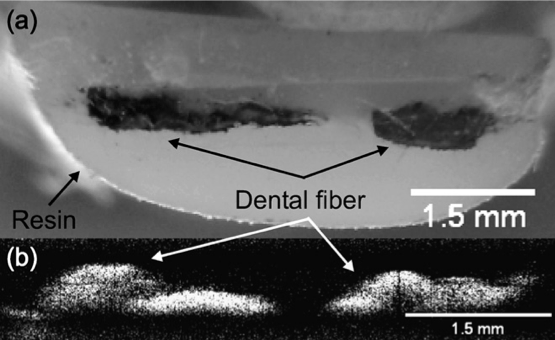
\includegraphics[height=4.6cm]{frc-1}
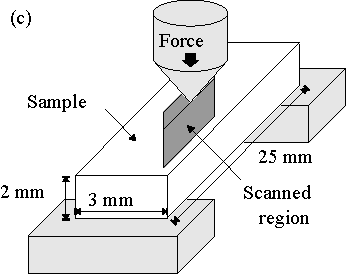
\includegraphics{FRC-setup}
\caption{(a) Photograph of a section of the FRC where we can see the dental fiber. (b) OCT image confirms the ability to see the substructure of the composite, resin boundary is not shown. Because of the refractive index of the resin the vertical dimensions inside sample need to be corrected by a factor of 1.5. (c) Three point loading schematics with scanned region indicated.\label{fig:FRC photo}}
\end{figure}

For the mechanical cycling, the specimens were tested in three point loading, depicted in figure \ref{fig:FRC photo}.c, in a universal testing machine (Kratos Equipamentos Industriais LTDA, SP, Brazil). The load was applied to standard bar specimens with a loading angle of 90\textdegree{}, a crosshead speed of 3.0 mm/min and the distance between the two supports was 8 mm. Cyclic loading was carried out to 100 cycles or until the specimens failed. figure \ref{fig:FRC before and after} a and b show the OCT images of the sample, for a particular cycling load of 60 N. The images were taken as schematized in figure \ref{fig:FRC photo}. Scanning was not straightforward because the cycling cracked the resin surface leaving particles that scattered the light obfuscating the region below the point of contact and often saturating the detector. 
\begin{figure}[h]
\centering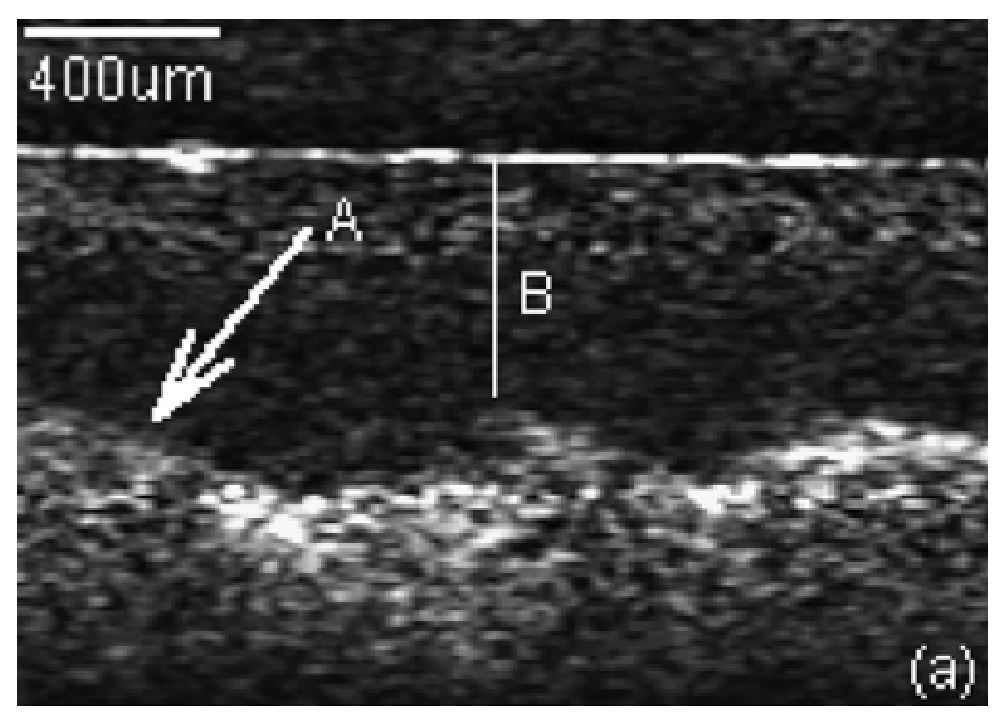
\includegraphics[height=4cm]{frc-2-a}
\centering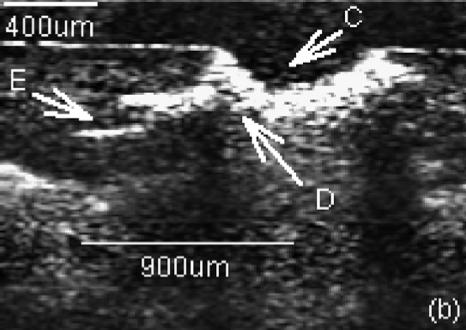
\includegraphics[height=4cm]{frc-2-b}
\caption{Slow crack growth (a) image is prior the cycling and (b) image after the cycling of 60 N load. (A) Dental fiber. (B) Distance from the surface of the beam to the top of the dental fiber. (C) Flaw initiation site. (D) Splinter region. (E) Hackle region.\label{fig:FRC before and after}}
\end{figure}

There are three characteristics regions surrounding the fracture origin on the fracture surface of brittle material. The first region is generally a relatively smooth (mirror) region, the second is a slightly stippled (mist) region and the third is a very coarse (hackle) region. This last region leads to macroscopic crack branching that is, the bifurcation of the main crack. The formation of these three regions occurs at a constant characteristic stress intensity factor\footcite{Mecholsky:1995p2523}. 

In figure \ref{fig:FRC before and after}.a, it is shown the OCT image prior the cycling. A indicates the image of dental fiber and B shows the distance from the surface of beam to the top of dental fiber (about 400 \textgreek{m}m). On the right hand side, figure \ref{fig:FRC before and after}.b, shows the results after cycling. We can note the extension of propagation about 900 \textgreek{m}m from the flow initiation site to the end of hackle region. This result demonstrates the possibility to study how crack initiates and propagates inside the dental material. It should be pointed out that, at 40 N load (not shown) the crack starts to form, but the resin is still intact. At 80 N load, the sample was fractured.

\subsection{Conclusions}

In conclusion, we have used the SDOCT technique to generate images of a FRC embedded in a composite resin. The results demonstrated the capacity of the OCT technique to generate images of the sites fracture initiation, crack propagation, and, regions surrounding the fracture. It is known that the penetration depth in real tooth can cover the whole enamel extension\footcite{DeMelo:2005p2100} and therefore imaging fiber to a 2 mm depth is feasible in real life. 

Since fracture is a major reason for clinical failure of dental restoration, and is generally preceded by slow crack propagation, the method shown here can be used for analysis of in-service failure of dental materials and, although it was only qualitatively analyzed here, it can be used in the future for quantitative analysis thus complementing other methods\footcite{Loughran:2005p2526}.


\section[Imaging of dentin and pulp chamber by OCT]{\emph{In vitro} Imaging of remaining dentin and pulp chamber by optical coherence tomography: comparison between 850 and 1280 nm}

Citotoxicity of the dental material, deep cavity preparation, and accidental exposition of pulp tissue are factors that can be involved with the pulp irritation. The OCT is a new modality of image capable to diagnose the complex dentin pulp and to produce images through the dentin substratum, being able to measure with precision the distance between the endings of the cavity to pulp chamber. OCT provided images into reminiscent dentinal to pulp cavity of about 1000 \textgreek{m}m (1280 nm) and 600 \textgreek{m}m (850 nm) in depth.

Before any restoring procedure, care must be taken to properly evaluate and protect the dentin and the pulp against physical, chemical, and bacterial aggressions. The protection strategies depend basically on the depth of the cavity, the age of the patient, the remaining dentin thickness, and the indicated restoring material. The depth is determined by the remaining dentin thickness between cavity floor and the pulp chamber's ceiling. The remaining dentin thickness of 500 \textgreek{m}m should be enough to protect the pulp tissue against the cytotoxic effects of dental materials\footcite{Hanks:1988p2379}, and the remaining dentin thickness of 300 \textgreek{m}m may provoke a persistent inflammatory pulpal response.

The OCT is a potential image technique that may contribute to prevent accidental pulp exposures in clinical practice and help pulp protection, by quantitatively determining the remaining dentin, thus helping to make the excavation procedures more predictable and safe.

During excavation procedures and cavity and crown preparation, the pulp may be accidentally exposed. Knowledge of the configuration of the pulpal space and the pulp-dentin complex morphology plays an important role to prevent iatrogenic or so-called accidental exposure of the pulp. It is often difficult in clinical practice and with conventional image techniques, such as X-ray, to identify the exact dimensions of the internal tooth anatomy\footcite{Mjor:2002p2276}.

To detect the depth of the dental cavity in relation to the pulpar chamber, the professionals withhold information collected through the clinical examination\textemdash visual and tactile inspection\textemdash and of the radiographic examination. These methods are subjective, which may lead to the wrong choice for the ideal treatment. Moreover, the radiographic procedure possesses some limitations for presenting overlapping of anatomical structures, for being a static method and emitting ionizing radiation.

More recently, besides evaluation of enamel interface restoration\footcite{DeMelo:2005p2100}, also early caries diagnostics\footcite{Freitas:2009p2142} and the analysis of the performance of the dental materials\footcite{Kyotoku:2007p788,Braz:2009p2143} have been studied and reported by our group. In 2006, Kauffman et al. performed the first OCT image of dental pulps using rat's teeth\footcite{Kauffman:2006p2144}.

%The key elements of an OCT setup include a broadband light source, whose spectral width limits the axial spatial resolution; an interferometer, which generally employs a Michelson design containing in one of the arms the sample and in the other arm a delay line; and an optical detector, whose signal output is electronically treated and fed to a computer for the image generation. Two domains can be exploited for implementation of an OCT system: the time domain or the spectral domain. In the time domain, the optical delay line arm basically consists of either a movable arm or a Fourier domain delay line\footcite{Cense:2004p2285}. In the spectral domain, there are no movable parts in the interferometer arms except for lateral displacement of the beam on the sample, and the recombined beams from the interferometer are sent to a spectrometer and are Fourier analyzed. It has been shown that spectral domain OCT SD-OCT has several advantages over the time domain OCT, including sensitivity\footnote{Wojtkowski:2002p3} and fast acquisition data, and because the first report on imaging implementation using SD-OCT\footnote{Wojtkowski:2002p3} it has been widespread. 

This work reports the first research comparing images obtained by OCT of the complex dentin-pulp of in vitro human teeth, using two different wavelengths in the near infrared, and also using a conical beam tomography as the gold standard. The results are compared, and the conclusion that OCT at 1280 nm performs better than at 850 nm is obtained, besides corroborating the feasibility of OCT for potential clinical use to prevent accidental exposure of the pulp and to promote preventive restoration treatment.


\subsection{Materials and methods}

The experimental study was carried out in accordance with the ethical guidelines in research with human participants by Center of Health Sciences, Universidade Federal de Pernambuco, Brazil. 

Higid molar teeth from humans were used in this research. The occlusal surfaces of the teeth were prepared with a perpendicular carbide bur along the axis of the teeth producing a plane on that surface, which were subsequently polished manually with a 400, 600, and 1200 sandpaper sheet. Wear was performed perpendicular to the long axis of teeth and lasted until the occurrence of minimal cavity pulpal exposure creating a plane on occlusal surface. The wear stopped until the occurrence of minimal cavity pulpal exposure. In practice, polishing or surface preparation is not required to obtain the images. 

The images of the remaining dentin thickness and pulp chamber were taken by scanning the occlusal surface in a vestibule-lingual direction. The laser penetrated into the teeth structure and a tomographic image of the frame, parallel to the axis of teeth was obtained. 

After the image construction by OCT 1280 and 850 nm, the teeth were tomographically analyzed using the i-CAT \gls{CBVT} imaging system Imaging Sciences International, LLC, Pennsylvania, which radiates from an X-ray source in a cone shape, encompassing a large volume with a single rotation about the sample. This tomography system is a technology used to analyze both double jaw anatomies in patients by dentistry when more accuracy is required on complementary exams. The CBVT produces volume imaging in an easier and faster way than conventional medical computed tomography\footcite{Danforth:2003p2286}. The scan offers times at 10, 20, and 40 s, with standard reconstruction taking <30 s, providing dentists with near-instant data for the best possible patient diagnosis, treatment, and surgical predictability. The pictures obtained are then reconstructed using algorithms to produce three-dimensional images at high resolution. Using the i-CAT software, it was possible to generate sliced 2-D images with thickness of 0.12 mm limited by the instrument resolution, eliminating the problem of superposition, and these images were then compared to the OCT images. 

\subsection{Results}
\begin{figure}[h]
\centering{}\input{debora-2.pdf_tex}
\caption{i-CAT cone beam volumetric tomography image of the dentin and pulp chamber studied: (a) 0.12 mm slice longitudinal of the tooth and (b) zoom 400\% at the dentin-pulp interface.\label{fig:i-CAT tomography}}
\end{figure}

For comparison purposes, we first show in figures \ref{fig:i-CAT tomography}.a and \ref{fig:i-CAT tomography}.b images by i-CAT CBVT of the pulp chamber region studied. The white area is the dentin (D), whereas the pulp chamber (PC) region is the dark area inside. The square region marked is the zoom region shown in figure \ref{fig:i-CAT tomography}.b. The dimensions in figures \ref{fig:i-CAT tomography}.a and \ref{fig:i-CAT tomography}.b are shown by the scales. figure \ref{fig:i-CAT tomography} shows a remaining dentin thickness of $\sim120$ \textgreek{m}m, which was thick enough to avoid pulpar exposition.
\begin{figure}[h]
\centering{}\input{debora-3.pdf_tex}
\caption{OCT images of the Dentin (D) and pulp chamber (PC) corresponding to the i-CAT CBVT image of fig. \ref{fig:i-CAT tomography}.b: (a) OCT at 1280 nm and (b) OCT at 850 nm. The black transversal region in (a) is an artifact (indicated by the arrow).\label{fig:OCT dentin pulp chamber}}
\end{figure}

The OCT images at the wavelengths of 1280 and 850 nm for the zoomed-in region shown in the i-CAT CBVT image of figure \ref{fig:i-CAT tomography}.b are seen in figures \ref{fig:OCT dentin pulp chamber}.a and \ref{fig:OCT dentin pulp chamber}.b, respectively, which also show the structural components of the pulp-dentin complex. The structures in the OCT images are distinguished due to the different gray levels (or blue levels, in the case of the 850 nm system), where the contour of the chamber to pulp appears whiter (highest scattered intensities) and the dentin with the darker level (lowest scattered intensity). Those structures are clearly delineated due to influence of the structure of the biological components with distinct refractive indices, which backscatters light in very different ways. No pulp exposition is observed, as confirmed by the i-CAT CBVT, and comparing figures \ref{fig:i-CAT tomography}.b, \ref{fig:OCT dentin pulp chamber}.a, and \ref{fig:OCT dentin pulp chamber}.b, it clearly demonstrates the capacity of quantitative measurement by the OCT with remaining dentin thickness measured as $\sim120$ \textgreek{m}m. Note that the measurements in the OCT value showed on the scale must be divided by the refraction index of dentin $\sim1.5$\footcite{Colston:1998p1677} The black transversal region, indicated by the arrow in figure \ref{fig:OCT dentin pulp chamber}.a, is an artifact.
\begin{figure}[h]
\centering{}\input{debora-4.pdf_tex}
\caption{Dentin (D), pulp chamber (PC), and site of the pulpal exposure (PE). Image of the pulp-dentin complex acquired with (a) i-CAT CBVT , (b) OCT 1280 nm image (c) OCT 850 nm image.\label{fig:pulp exposure}}
\end{figure}

Figure \ref{fig:pulp exposure} shows an image where the exposition of the pulp cavity is clearly seen. Figure \ref{fig:pulp exposure}.a is the i-CAT CBVT image section, figure \ref{fig:pulp exposure}.b the OCT at 1280 nm, and figure 4(c) the OCT at 850 nm. Once again, D and PC are clearly delineated in the OCT image. The pulp exposition site (PE) is seen as a discontinuity at the dentin surface, which is the homogeneous white line of high intensity. The OCT images shown allow the direct measurement of the observed region depth.
\begin{figure}[h]
\centering{}\input{debora-5.pdf_tex}
\caption{Image of the deeper pulp ceiling visualized by the OCT. (PC) beginning of the contour of the pulpar ceiling, (D) dentin: (a) 1000 \textgreek{m}m visible depth of the pulp cavity at 1280 nm. The black transversal region is an artifact (b) 600 \textgreek{m}m visible depth of the pulp cavity at 850 nm.\label{fig:deep ceiling}}
\end{figure}

In order to verify the maximum depth that could be achieved for each OCT system, we carried out a series of measurements whereby the studied dentin region was being reduced by polishing until the pulp could be identified. The scale shown in figures \ref{fig:deep ceiling}.a and \ref{fig:deep ceiling}.b clearly demonstrate the capacity of quantitative assessment of the OCT, as well as the maximum penetration depth of the radiation inside of the dentin region. Comparing the measurements of the deeper ceiling of the pulp chamber visualized at the two different wavelengths 1280 and 850 nm, respectively, the remaining measured dentin thickness was $\sim1000$ \textgreek{m}m at 1280 nm and 600 \textgreek{m}m at 850 nm system. These values had already been corrected for the dentin refractive index $\sim1.5$\footcite{Colston:1998p1677}.

The deeper penetration depth of the light at 1280 nm compared to 850 nm is due to a reduction of absorption and scattering coefficients of the dentin at 1280 nm\footcite{Drexler:2004p1728}.
\begin{figure}[h]
\centering{}\input{debora-6.pdf_tex}
\caption{OCT image composition showing the dentin (D) and pulp chamber (PC2 and PC2) with wavelength of 1280 nm. Notice the thin layer of remaining dentin about 260 \textgreek{m}m to PC1 and 600 \textgreek{m}m to PC2.\label{fig:image composition}}
\end{figure}

As a final example, figure \ref{fig:image composition} shows a composition of three different images from OCT at 1280 nm, taken at the same sample, showing the view of the longitudinal slice detecting cusps (C), D, and the vestibular and palatine pulp horn, where it is possible to identify a remaining thin layer of dentin of roughly 260 and 600 \textgreek{m}m (PC1 and PC2) between the cavity floor and pulp chamber. This is another clear demonstration of the potential of OCT for pulp chamber assessment.

\subsection{Conclusion}

The OCT clearly demonstrate the capacity of quantitative assessment and penetration of the radiation on the pulp chamber and the remaining dentin, compared to the scan in i-CAT CBVT. In accordance with the results presented for the OCTs with a wavelength of 1280 and 850 nm, the two techniques presented effectiveness. Furthermore, our experiment corroborated the depth of penetration almost two times bigger for 1280 nm OCT. OCT is a non-invasive and non-destructive technique; as a consequence, it possesses great potential to be used routinely in clinical practice for the diagnosis of the complex dentin pulp, preventing accidental exposure of the pulp and promoting preventive restoration treatment. For practical use, a hand piece or an appropriate head for the imaging acquisition is required, which is a technologically solvable issue.

\section[Clinical use of OCT to evaluate integrity of dental restorations]{Clinical use of optical coherence tomography to evaluate the integrity of dental restorations}

We have applied Optical Coherence Tomography (OCT) clinically to assess dental restorations in humans. Twenty patients with resin composite restorations in anterior teeth were selected and evaluated using a conventional radiographic examination, visual inspection and OCT. Images were obtained using a home built OCT system operating in the spectral domain, with an 850 nm superluminescent diode light source. The results were analyzed with respect to the integrity and marginal adaptation of the restoration. Using appropriate software failed and failing restorations, including those with lesioned regions, could be located prior to the placement of a new restoration. Lesions and failed restorations were identified with the OCT system that could not be seen by conventional visual and X-ray examinations and these were found to be present on surgical intervention. This in vivo study demonstrates that the OCT technique has a great potential to be used in clinical practice to assess dental restorations and prevent recurrent caries. 

\subsection{Introduction}

%In recent years, several methods using light have been proposed to address the need for better detection and diagnostic tools in dentistry. Digital imaging fiber-optic transillumination (DIFOTI), multi-photon imaging, quantitative light fluorescence (QLF), infrared fluorescence (DIAGNOdent), infrared thermography, Raman spectroscopy, optical coherence tomography (OCT) and terahertz imaging are a few techniques that are currently under evaluation for improved diagnosis\footcite{Hall:2004p1838,Fried:2005p1836,Alex:2005p1695,ChooSmith:2008p1834}.

%The first study applying OCT to be carried out in Dentistry, both in vitro and in vivo, was in 1998, using a prototype handpiece for the characterization of both hard and soft dental tissues \footcite{Colston:1995p1719,Feldchtein:1996p111}. In 2003, a commercial prototype OCT system was adapted to a commercial surgical microscope to perform in vitro and in vivo images of carious lesions and restorations \footcite{Brandenburg:2003p2055}. OCT has also been employed for the early detection of oral cancer \footcite{Jung:2005p2056}. In vitro studies evaluating enamel interface restoration \footcite{DeMelo:2005p2100}, early caries diagnostics \footcite{Freitas:2009p2142}, and analysis of the performance of dental materials\footcite{Braz:2009p2143} have also been reported. In 2006, the first OCT image of dental pulp was performed using rat's teeth \footcite{Kauffman:2006p2144}. Recently, remaining dentin and the pulp chamber from human teeth were also imaged by OCT in vitro as reported in \footcite{Fonseca:2009p1}. Endodontic applications of OCT have been explored in order to evaluate root canals \footcite{Shemesh:2007p1843} and Sinescu and co-workers used OCT to investigate the marginal adaptation of fixed dental prosthesis before installing them in patients \footcite{Sinescu:2009p2146}. However, little work has been reported on OCT being used in a clinical setting as part of a clinical evaluation, specifically looking at restoration integrity.

Dental restorations provide a barrier restricting oral fluids and bacteria from entering the tooth after the removal of any damaged or missing tissue. An inadequate marginal seal can result in gap formation that leads to microleakage, which may be responsible for marginal breakdown, recurrent caries, increased post-operative sensitivity, pulpal inflammation, and staining \footcite{Attar:2008p2147}.

The success of the restorative treatment depends on the integrity of the tooth-restoration interface and this particular region is the subject of much research and discussion in the Dental community. Clinically, the most common tools for detection of restorative failures are by tactile, visual inspection or radiographic examination. However, since initial microleakages can be clinically and radiographically imperceptible, secondary caries may currently progress before the problem can be detected by the dental practitioner.

Here we present an \emph{in vivo} study to detect failures at the enamel-dental restoration interface, and the integrity of superficial and internal structures of restorations in a clinical setting using OCT. This study was undertaken with 20 patients attending the Dentistry College of the Universidade Federal de Pernambuco. The relatively large number of attending patients allowed us to obtain and analyze the results in a very consistent manner. Results were compared to conventional radiographs and clinical examination, represented here by photographs. 

\subsection{Material and methods}

This study was developed according to the guidelines given by Ethical Committee in Human Research of the Universidade Federal de Pernambuco, Brazil. Twenty patients with resin composite restorations in upper anterior teeth were selected. These patients were between 18 and 45 years old, both male and female, and had their restorations performed between 1999 and 2009. All the restorations had a superficial satisfactory clinical aspect with no obvious aesthetic failures such as staining, undesirable shape or obvious missing material.
\begin{figure}[h]
\center{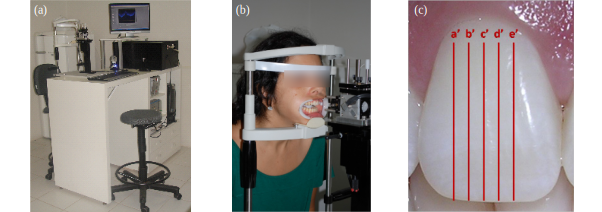
\includegraphics[height=6cm]{claudiaFig1}}\caption{(a) SDOCT adapted for clinical essays; (b) Positioning the patient; (c) Sequence indicating the scan positioning in the patient's teeth. identifying the tomographic slices.\label{fig:clinical photos}}
\end{figure}
 
To perform the OCT examination, a lip retractor was used on the patients, and their heads were positioned in an appropriate support, in front of the sample arm, seen in figures \ref{fig:clinical photos}.a and \ref{fig:clinical photos}.b. The image acquisition time is less than one second (for each image, there was 0.1 second of pre-scan settling time and 80 \textgreek{m}s of integration time) though the support was used to minimize movement which would otherwise blur the high optical resolution images. The authors analyzed the results with respect to the integrity and marginal adaptation of the restoration by visual inspection of the images in real time as well as on the images produced from the subsequent image processing.

As comparison criteria to OCT, we employed the diagnostic methods most widely used in dentistry: a clinical examination composed of visual and/or tactile inspection (shown in this paper by photographs) and a conventional X-ray. The dental X-Ray equipment used was the Spectro 70X (Dabi Atlante), operating at 70 kVp head power and a head current of 8 mA. The radiographic film used was Kodak Dental Intraoral E-Speed Film (Carestream Health), and the dental developer and fixer, was from the same manufacturer.

During a clinical examination, it is possible to detect changes in resin composite color, polishing failures, contact point problems and major gaps and fissures; radiographic images can show excess or lack of restorative material, large areas of demineralization (typically greater than 30\% of mineral loss), and gaps or fractures points larger than the minimum detection size observed by OCT.

To evaluate the presence, or otherwise, of failures in the restorations, three experienced professionals, all of them Restorative Dentistry professors, were trained to interpret OCT images. Each professor was then individually shown the clinical photograph of each restoration in question, and requested to complete a form describing what they could see in that patient's image in terms of the restoration extension, and if there was any form of failure. In case of detected failure they were then asked to classify the failure. Then, the radiographic images were shown, in the same way and, last, the OCT images. To analyze the data a Kappa coefficient test was applied. Kappa coefficient is a statistical measure of the agreement for qualitative/categorical items; its aim is not to compare the diagnostic potential between the three techniques employed, but to compare how the evaluators agree among themselves in each form of diagnostic technique separately. After the analysis all of the patients that presented failures in their restorations were recalled to the clinic and had new procedures performed after a discussion with the patient following the approved clinical procedure.

\subsection{Results}

Table \ref{table:preliminary results} indicates a comparison between all the methods used in this work for the first three cases.
\begin{table}[H]
\noindent \begin{centering}
\begin{tabular}{ccccc}
\hline 
Patient \# & %
\begin{minipage}[t]{0.15\linewidth}%
Visual inspection defect%
\end{minipage} & %
\begin{minipage}[t]{0.15\linewidth}%
X-Ray exam defect%
\end{minipage} & %
\begin{minipage}[t]{0.1\linewidth}%
OCT defect%
\end{minipage} & Comment\tabularnewline
\hline
\hline 
1 & No & No & No & %
\begin{minipage}[t]{0.4\linewidth}%
A well placed and sound restoration%
\end{minipage}\tabularnewline
2 & No & No & Yes & %
\begin{minipage}[t]{0.4\linewidth}%
From a visual inspection, is only possible to observe that the restoration
is not polished%
\end{minipage}\tabularnewline
3 & No & Yes & Yes & %
\begin{minipage}[t]{0.4\linewidth}%
X-ray exam only shows the excess of restorative material, but is not
able to visualize the failures seen by OCT%
\end{minipage}\tabularnewline
\hline
\end{tabular}\caption{A summary of the preliminary results.\label{table:preliminary results}}
\par\end{centering}
\end{table}

Figure \ref{fig:good restoration} shows a sequence of examinations of a patient with a well placed and sound restoration in a central incisor, placed seven years previously. Figure \ref{fig:good restoration}.a represents the clinical examination; \ref{fig:good restoration}.b, the conventional radiograph showing the restoration at the incisal region in the circle. Arrows in \ref{fig:good restoration}.c indicate the interface between the enamel and the restorative material, which can be clearly seen.
\begin{figure}[h]
\noindent \centering{}\input{claudiaFig4.pdf_tex}
\caption{Well suited restoration of a central incisor. (a) clinical photograph; (b) conventional radiography; (c) sequence of OCT images: arrows indicate the integrity in the enamel-restoration interface.}
\label{fig:good restoration}
\end{figure}

Figure \ref{fig:aesthetic}.a shows a lateral incisor with an aesthetic facet (not polished) over an incisal and cervical restorations, confirmed by radiography in figure \ref{fig:aesthetic}.b, performed two weeks before the analysis reported here. In the OCT image, figure \ref{fig:aesthetic}.b, an air bubble in the restoration (within the circle) can be seen and the dots indicate the points of microleakage at the enamel-restoration interface. The small rectangles indicate an extensive space under the restoration, probably due to resin polymerization contraction during the restorative procedure and the triangles indicate crack points between resin increments.
\begin{figure}[h]
\noindent \begin{centering}
\input{claudiaFig5.pdf_tex}\caption{An aesthetic facet over an incisal restoration. (a) clinical photograph; (b) conventional radiography; (c) sequence of OCT images: air bubble (shown within the major circle); gaps at the interface enamel-restoration (indicated by the dots); small rectangles indicate an space under the restoration, probably due to polymerization\label{fig:aesthetic}}
\par\end{centering}
\end{figure}

Restorations involving medium and incisal regions of a central incisor, performed in 2001 in another patient are shown in figure \ref{fig:medium region}, where figure \ref{fig:medium region}.a shows the clinical photograph with no sign of failure, and different colors between the resin composite and the dental enamel. In figure \ref{fig:medium region}.b, the conventional radiograph, it is possible to observe excess restorative material at proximal surfaces; and figure \ref{fig:medium region}.c shows the OCT image sequence. The arrow here indicates the well placed enamel-restoration interface. However, several undesirable features can be identified: air bubble (within the circle); evidence of a gap between the enamel and the restorative material (identified by the dots); superficial defects and internal fractures in the resin composite (identified by the triangles).
\begin{figure}[h]
\noindent \centering{}
\input{claudiaFig6.pdf_tex}\caption{Restoration involving medium and incisal regions. (a) clinical photograph; (b) conventional radiography; (c) sequence of OCT images: arrow indicates the well suited enamel-restoration interface; within the circle, an air bubble; dots indicate gaps at the enamel-restoration interface; triangles shows superficial defects and internal fractures at the resin composite; stars indicate imaging artifacts.}
\label{fig:medium region}
\end{figure}

In some cases, a restoration does not necessarily need to present failures throughout its entire structure to be considered for replacement and they may well show one part which is well placed and intact whilst another area has problems. This can also be seen in figures \ref{fig:medium region}.c and \ref{fig:7}. In the first slice of figure \ref{fig:medium region}.c, we can see an arrow that indicates the well placed enamel-restoration interface, but in subsequent slices, we can see some failures, described previously. The same situation can be seen in figure \ref{fig:7}, with a restoration involving medium and incisal regions. Arrows indicate the well placed enamel-restoration interface; dots indicate enamel-restoration microleakages; triangles indicate evidence of superficial fissures at the resin composite; another feature is the different pseudo color of the resin composite at the incisal region when compared to medium region, marked with the large rectangles. This can be seen by OCT because lighter colors of resin have lower refractive indices, and thus this modifies the scattering in this region. In figure \ref{fig:8}, we can see a sequence of failures over the entire structure of an incisal restoration (dots), beside the enamel-dentin junction.
\begin{figure}[h]
\begin{minipage}[t]{0.54\textwidth}
\centering
\input{claudiaFig7.pdf_tex}
\caption{Restoration involving medium and incisal regions. Arrows indicate the well suited enamel-restoration interface; dots, the presence of gaps; triangles demonstrate superficial fissures at the resin composite; within the large rectangle, we can observe a darker region, corresponding to lightest resin color increment in the incisal part of the restoration.}
\label{fig:7}
\end{minipage}
\hfill
\centering
\begin{minipage}[t]{0.44444\textwidth}
\input{claudiaFig8.pdf_tex}
\caption{Sequence of an incisal restoration with defects throughout the entire structure. Dots indicate gaps between the restorative material and the dental enamel; in DEJ, we can observe the dentin-enamel junction; artifact imaging indicated by star.}
\label{fig:8}
\end{minipage}
\end{figure}
Finally, in figure \ref{fig:9}, we can observe three different aesthetic facets. In the region indicated by the diamonds, problems with the cervical adaptation of the restorations are identified in figures \ref{fig:9}.a and \ref{fig:9}.b, whereas a well suited adaptation is seen in figure \ref{fig:9}.c. None of these clinically important defects, seen by OCT, could be observed in the clinical images and X-rays, even when they were subsequently examined after the detecting a problem in the OCT data sets.
\begin{figure}[h]
\centering
\input{claudiaFig9.pdf_tex}
\caption{Three different aesthetic facets. Diamonds indicate problems with cervical adaptation of the restorations in a) and b), and a well suited adaptation in c).} 
\label{fig:9}
\end{figure}
\begin{table}
\noindent \centering{}\begin{tabular}{ccccc}
\hline 
 & & Clinical exam & Radiographic & OCT\tabularnewline
\hline
\hline 
$\kappa$ & & 0.732 & 0.732 & 1.000\tabularnewline
p-value & & <0.001 & <0.001 & <0.001\tabularnewline
$\kappa$ 95\% range trust & Upper & 1.000 & 1.000 & 1.000\tabularnewline
 & Lower & 0.374 & 0.374 & 0.642\tabularnewline
\hline
\end{tabular}\caption{Kappa coefficient results.\label{table:kappa results}}
\end{table}

Table \ref{table:kappa results} shows the Kappa coefficient results for each form of diagnostic examination. It can be seen that for clinical and radiographic examinations there was a substantial agreement between the evaluators, whilst for the OCT examinations the Kappa index obtained demonstrates perfect agreement: it means that the OCT images provide more accurate information to diagnostic than the clinical photographs and the X-ray exam. It was not possible to compare the kinds of failures seen in each type of examination, as the OCT is able to visualize internal structures that are impossible to be seen in the clinical inspection or radiographic examination.

\subsection{Discussion}

The improvements in the aesthetic and physical properties of composite resins over the past ten years have established them as the material of choice for restorations of anterior teeth when used in conjunction with the acid-etch technique and dental bonding systems\footcite{Garoushi:2007p2191}. However, their high aesthetic quality frequently makes it harder to see early signs of failure and due to the way that these materials behave, compared to traditional amalgam and gold restorations, early failure is more likely. Failures at the tooth-restoration interface can be associated with several factors including incorrect restorative technique, the physical properties of the materials used and, especially, the contraction of the material generated during the polymerization of the restorative material.

An adequate marginal adaptation and the integrity of the restoration are fundamental to the success of the dental treatment: failures in the marginal surface cause microleakage and bacteria infiltration; loss of integrity can be present in the internal or superficial structure of the restoration, and reduces the quality of the restoration, leading to early fracture of the restorative treatment. Some defects seen in this study are known to cause a loss of integrity in resin based composite restorations including air bubbles in the restoration, regions without material under the restoration (voids), cracks and fissures at the resin composite and gaps. When these kinds of failures are present and the restorative procedure is not adequate, a new treatment should be discussed with the patient.

%Previous studies have shown some defects we have identified in this paper: the dentin enamel junction was evidenced by several authors\footcite{Colston:1995p1719,Feldchtein:1996p111,Brandenburg:2003p2055}; Melo et al (2005)\footcite{DeMelo:2005p2100} presented induced marginal microleakage; Sadr et al (2009)\footcite{24} had shown the evolution of a marginal microleakage to a secondary caries with absence of restorative material under the restoration; the absence of restorative material in the interface between the restoration and the dental tissue (similar to that we have shown in figure 5), presence of gaps, as well as crack points of the restorative material were presented by Negritu et al (2009)\footcite{Negrutiu:2009p2189}; air bubble and gaps were also presented in the study performed by Feldchtein et al (1998)\footcite{Feldchtein:1996p111} and, finally, crack propagation into the resin composite was described by Braz et al (2009)\footcite{Braz:2009p2143}.

The current methods clinically used to diagnosis are not able to visualize micrometric structures. In the radiographic examination, for example, an early enamel caries lesion is visible only after approximately 30\%\textendash{}40\% mineral loss\footcite{White:2000p2224}. This deficiency makes it difficult to diagnose early recurrent caries, when an earlier diagnosis means an easier and less traumatic treatment, leaving more enamel present in the tooth after treatment.

The Kappa coefficient was applied to analyze the concordance index of the diagnosis of the professionals selected for each examination modality separately, and the OCT method demonstrated perfect agreement between the evaluators, while there was a substantial agreement for the clinical and radiographic examinations. This indicates that OCT, besides be a good tool for diagnosis can be consistently interpreted by well trained dentists. However, it was not possible to use a statistical test to compare the clinical, X-ray and OCT examinations simultaneously. The first method (clinical observation) is only able to see defects at external surfaces; radiographic methods image across the tooth, but the resulting image inherently overlays the buccal and lingual 14 surfaces making it difficult to detect and determine internal problems. OCT can produce two dimensional and cross-sectional images, allowing the observer to see external and internal details, without overlap of structures, being able to accurately locate the visualized structures. Thus teeth were visualized in different forms in each type of examination, but many of the minor defects (air bubbles, for example) only can be seen by OCT. However, all defects detected by clinical and X-ray examinations were also detected using the OCT protocol.

This study demonstrates that OCT is a powerful tool for the early detection of failures on restorations, through visualization of microleakages, internal fractures, superficial cracks and fissures, tooth demineralization under the restorative material and cervical adaptation of the restorations. Incipient lesions can be precisely located, their depth may be measured and their proximity to the dentin-enamel junction may be determined. The sensitivity of the OCT technique is sufficient such that details, including the use of different colors of resin composite used to increase the esthetic aspect of a restoration, can be identified due to the slightly different scattering properties (see figure \ref{fig:7}.

As dentists are used to dental radiographs for diagnostic purposes, OCT imaging, which shows similar dental morphology, could be readily adopted\footcite{ChooSmith:2008p1834} and, ideally, the number of conventional X-ray investigations would be reduced in order to minimize the patients exposure to ionizing radiation\footcite{Brandenburg:2003p2055}.

However, it is necessary to recognize some limitations of OCT: the system has a small depth penetration, (1-3 mm in teeth), which is, however, adequate for enamel and even dentin visualization. This is partly because we chose to use light at 850nm in order to increase the contrast between areas with only slightly different scattering properties. The use of longer wavelength sources (around 1300nm), with some slight loss of contrast, and hence sensitivity, may provide the best compromise between depth of imaging and sensitivity to minor alterations in structure. Furthermore, our current system does not allow the use of the technique in every tooth, just on incisors and canines. Thus for this first stage of our studies applying OCT in vivo, we only assessed anterior teeth, for two reasons: incisors and canines are the teeth that require better esthetic restorative procedures, and the unavailability of a handpiece probe, presently under development, to reach the posterior dentition.

Some difficulties were found during the data collection of this study: the major of them was to control the production of saliva and subsequent patient movement, which tended to produce image artifacts. Thus was minimized by careful explanation to the patient and the use of the stabilization bar. A further complication was to undertake the examinations in patients presenting a maxillary overjet (an orthodontic condition in which the third incisor is ahead of the cervical third in the upper incisors, and thus the teeth appear to be inclined horizontally) \textendash{} this problem was solved by requesting the patient to bow their head slightly but, in a long term, the solution is in the development of a handpiece probe.

Further clinical studies covering cervical adaptation of aesthetics-facets and fixed crowns are currently underway. The high sensitivity of OCT to minor defects also opens up a further clinical question over which minor defects will progress to server complications and which may stay at the minor level. The development of such revised treatment protocols is beyond the scope of the present study but it is an area that will need to be investigated as OCT moves towards a standard diagnostic instrument in clinical practice, as is the case with any new technological advance.

\subsection{Conclusion}

Compared to conventional radiography, OCT is a powerful tool for investigation of failures at the tooth-restoration interface. OCT is able to exactly visualize external and internal micrometric structures, not perceived by clinical examination or conventional radiography, proving its superiority as a technique for early diagnosis of restoration failures and prevention of recurrent caries. However, because of the low penetration depth of OCT, conventional radiography imaging may not be totally substituted. This was a qualitative study applying OCT in dental clinics; we used conventional X-Ray, the most widely used modality of imaging for diagnostic assessment in dental clinics, and the clinical examination as the comparison for our study. We analyzed the differences between the modalities of exams mentioned above and the advantages and limitations of conventional radiography and OCT examinations. Besides other applications of the OCT technique in vivo, further complementary studies are under-way to determine dental composites failures in a quantitative manner, as well as their size or extent.

%%%%%%%%%%%%%%%%%%%%%%%%%%%%%%%%%%%%%%%%%%%%%%%%%%%%%%%%%%%%%%%%%%%%%%%%%%%%%%%%%%%%%%%%%%%%%%%%%%%%%%%%%%%%%%%%%%%%%%%%%%%
%\part{Optics on chip}
\chapter{Photonics Integrated Circuits}


It is unnecessary to emphasize the importance of electronics integrated circuits to the current world. But it is worth to investigate if it is possible to create the same structure in different fields. In this investigation one can notice the two crucial feature of the success. The use of massively parallel device patterning enabled by photolithography and the search to decrease device size to its physical limits.

Three ramification using the micro-fabrication process have come of age in the last decade: Microfluidics, micro-mechanical devices (MEM) and integrated optics. Microfluidics enables the possibility of massive chemical analysis which revolutionized genetic research, enabling operation such as DNA sequencing to be performed at a fraction of time that was done before. Integrated optics which has the potential of large bandwidth data transfer and spectroscopic analysis, and possibly quantum processing.

Making use of this maturity, we started an effort for the integration of a optical coherence tomography system in a single chip. From here we report the results of such efforts. 

\section{Broad picture}

The platform in which integrated photonic circuits works consists in the use of a high index of refraction material surrounded by a material with lower index of refraction. This structure enables the most basic feature needed in the development of photonic integrated circuit which is to trap light in a single layer, in this case the higher refractive index dielectric, and to easily create lane where we can guide this light anywhere we want. We call this platform a \gls{slab waveguide}. Light that is guided in the higher index material can be treated as a two dimensional wave, and a rigorous description to the waveguide is given in section \ref{section:slab waveguide}. In this regime, knowledge of free space optics, appropriately adapted to two dimensions, can be applied to design photonic devices. Components like lenses, mirrors, concave mirrors, prisms, gratings can be readily visualizable.

A good platforms also needs a way to be manufactured. In this regard, PICs are fortunate to be able to share the same platform as electronic integrated circuit, silicon-on-insulator, and therefore it can leverage all its fabrication and patterning know-how and infrastructure. Silicon has an index of refraction of 3.5 at wavelength 1500 nm together with its low index medium friend silicon dioxide, with 1.5 at 1500 nm. They make an excellent high index contrast composite that allows high light confinement increasing circuit compactness.

Another component is wire waveguide, where a high index of refraction material is surrounded by lower index material in two dimension. This structure transport light like electrons on copper wire. This structure is widely used as fiber optics, where system built on fiber optics can implemented on chip waveguides.

%Attempts to fabricate on commercial foundries has been made\footcite{Orcutt:2008p1769}


\section{Slab waveguide}
\label{section:slab waveguide}

%
\begin{figure}[h]
\noindent \centering{}\includegraphics[scale=0.8]{figures/slab}\caption{}

\end{figure}
We define slab waveguide as medium comprised of an infinite film (which will be refereed as core) of thickness $h$ and index of refraction $n_{f}$. This film was laid over a substrate with index of refraction $n_{s}$ and covered with a material with index of refraction $n_{c}$. The guiding film (core) have a index of refraction greater than both the substrate and the cover, or more exactly $n_{f}>n_{s}\ge n_{c}$. The index of refraction field can be written as
\begin{equation}
n\left(z\right)=\begin{cases}
n_{c}, & z\ge h\\
n_{f}, & 0<z<h\\
n_{s}, & z\le0\end{cases}.\label{eq:refractive index}\end{equation}
Over this field Maxwell's equations shown here assuming a harmonic mode with angular frequency $\omega$ and magnetic permeability uniform and equal $\mu_{0}$.
\begin{subequations}\begin{eqnarray}
\nabla\cdot\epsilon\mathbf{E} & = & 0,\label{eq:maxwell 1}\\
\nabla\cdot\mathbf{B} & = & 0,\label{eq:maxwell 2}\\
\nabla\times\mathbf{E} & = & i\omega\mathbf{B,}\label{eq:maxwell 3}\\
\nabla\times\mathbf{B} & = & i\omega\epsilon\mathbf{E}.\label{eq:maxwell 4}\end{eqnarray}
\label{eq:maxwell}\end{subequations}
From these equation the following wave equations can be derived
\begin{subequations}\begin{eqnarray}
\nabla^{2}\mathbf{E}+k^{2}\mathbf{E} & = & 0,\label{eq:wave equation E}\\
\nabla^{2}\mathbf{B}+k^{2}\mathbf{B} & = & 0,\label{eq:wave equation B}\end{eqnarray}
\label{eq:wave equation}\end{subequations}
where, $k=\frac{2\pi}{\lambda}=\frac{\omega}{c}$. The medium we are dealing with is has a symmetry by translation on the $x$ and $y$ axis. This allow us to have a solution in the following forms
\begin{eqnarray}
\mathbf{E}\left(\mathbf{R}\right) & = & \Psi\left(\mathbf{r}\right)\mathbf{\Phi}\left(z\right)\label{eq:assumption E}\\
\mathbf{B}\left(\mathbf{R}\right) & = & \Psi\left(\mathbf{r}\right)\mathbf{\Phi}\left(z\right)\label{eq:assumption B}\end{eqnarray}
where $\mathbf{r}=x\hat{i}+y\hat{j}$, $\Psi\left(\mathbf{r}\right)$ is a scalar field that depends only on $\mathbf{r}$, and $\mathbf{\Phi}\left(z\right)$ is a vector field that depends only on $z$, notice that is $\mathbf{\Phi}\left(z\right)$ that carries the field direction information. Either assumption can be used. Naturally the electric and magnetic field are still connected through Maxwell equations \ref{eq:maxwell 3} and \ref{eq:maxwell 4}, properly rewritten below
\begin{subequations}\begin{eqnarray}
\mathbf{B} & = & \frac{1}{i\omega}\nabla\times\mathbf{E},\\
\mathbf{E} & = & \frac{\epsilon\mu}{i\omega}\nabla\times\mathbf{B}.
\end{eqnarray}\end{subequations}

We can break down the nabla into an in-plane ($\nabla_{t}^{2}$) and a transversal to the plane ($\frac{\partial^{2}}{\partial z^{2}}$) component as $\nabla^{2}=\nabla_{t}^{2}+\frac{\partial^{2}}{\partial z^{2}}$, and separating variable we get
\begin{equation}
\frac{1}{\mathbf{\Phi}\left(z\right)}\frac{\partial^{2}\mathbf{\Phi}\left(z\right)}{\partial z^{2}}+\frac{1}{\Psi\left(\mathbf{r}\right)}\nabla_{t}^{2}\Psi\left(\mathbf{r}\right)-k^{2}n_i^{2}=0,
\label{eq:wave equation variables separeted}\end{equation}
defining
\begin{equation}
\frac{\partial^{2}\mathbf{\Phi}\left(z\right)}{\partial z^{2}}-\kappa_i^{2}\mathbf{\Phi}\left(z\right)=0\label{eq:out plane wave equation}\end{equation}
\begin{equation}
\nabla_{t}^{2}\Psi\left(\mathbf{r}\right)-\beta_i^{2}\Psi\left(\mathbf{r}\right)=0\label{eq:in plane wave equation}\end{equation}
using this definitions on \ref{eq:wave equation variables separeted}, we get
\begin{equation}
\kappa_i^{2}+\beta_i^{2}=k^{2}n^{2}.
\label{eq:kappa beta wavenumber relation}
\end{equation}

From equation \ref{eq:in plane wave equation}, shows that in the plane the electromagnetic field behaves like a bi-dimensional wave with wave number $\beta$. In the direction orthogonal to the plane we have a one-dimensional wave equation, with potential defined by the index of refraction. For the refractive index considered in our case, the potential is a \href{http://en.wikipedia.org/wiki/Finite_potential_well}{potential well}. Equation \ref{eq:out plane wave equation} is actually a set of three equations, that can be divided in two categories, one deals with the component in the direction normal to the interface, denoted here as $z$, and two that deal with components parallel to the interface surface
\begin{subequations}\begin{eqnarray}
\frac{\partial^{2}\Phi_{z}\left(z\right)}{\partial z^{2}}-\kappa_i^{2}\Phi_{z}\left(z\right) & = & 0,\label{eq:wave equation zz}\\
\frac{\partial^{2}\mathbf{\Phi}_{t}\left(z\right)}{\partial z^{2}}-\kappa_i^{2}\mathbf{\Phi}_{t}\left(z\right) & = & 0,\label{eq:wave equation zt}
\end{eqnarray}\end{subequations}
where as before, $i$ depends on the range of $z$. The linkage between neighboring ranges are described by the boundary conditions
\begin{subequations}
\begin{eqnarray}
\hat{n}\cdot\left(\epsilon_{a}\mathbf{E}_{a}-\epsilon_{b}\mathbf{E}_{b}\right) & = & 0\label{eq:boundary conditions 1}\\
\hat{n}\cdot\left(\mathbf{B}_{a}-\mathbf{B}_{b}\right) & = & 0\label{eq:boundary conditions 2}\\
\hat{n}\times\left(\mathbf{E}_{a}-\mathbf{E}_{b}\right) & = & 0\label{eq:boundary conditions 3}\\
\hat{n}\times\left(\frac{1}{\mu_{a}}\mathbf{B}_{a}-\frac{1}{\mu_{b}}\mathbf{B}_{b}\right) & = & 0,\label{eq:boundary conditions 4}\end{eqnarray}
\label{eq:boundary conditions}\end{subequations}
where $a$ and $b$ can be either $s,f$ or $c$. Using the assumption \ref{eq:assumption E}, these boundary conditions can be shown to be equivalent to
\begin{subequations}\begin{eqnarray}
n_{j}^{2}\Phi_{jz} & = & n_{k}^{2}\Phi_{kz}\label{eq:boundary Ez}\\
\frac{\partial\Phi_{jz}}{\partial z} & = & \frac{\partial\Phi_{kz}}{\partial z},
\label{eq:boundary dEz}\end{eqnarray}
\label{eq:boundary E}\end{subequations}
where we did not show the equivalent boundary conditions for the tangential components $\mathbf{\Phi}_{t}$. Applying the boundary conditions on $\mathbf{\Phi}_{t}$ will gives us a solution that is linearly independent to the solution of $\Phi_{z}$. Although it is possible to obtain this second solution, it is easier make the assumption \ref{eq:assumption B} and apply the boundary conditions, which this time will give rise to
\begin{subequations}
\begin{eqnarray}
\Phi_{jz} & = & \Phi_{kz}\label{eq:boundary Bz}\\
\frac{\partial\Phi_{jz}}{\partial z} & = & \frac{\partial\Phi_{kz}}{\partial z}.\label{eq:boundary dBz}\end{eqnarray}
\label{eq:boundary B}\end{subequations}
The wave equation \ref{eq:wave equation zz}, with the potential \ref{eq:refractive index}, connected by conditions \ref{eq:boundary E} is the problem of the wave in a square well. For a chosen value of $k$, continuous values of $\kappa$ and therefore $\beta$ exists. But for values of $\kappa$ that solves the equation
\begin{equation}
\tan\left(h\kappa_{f}\right)=\frac{\kappa_{c}+\kappa_{s}}{\kappa_{f}\left[1-\frac{\kappa_{c}\kappa_{s}}{\kappa_{f}^{2}}\right]}
\label{eq:TE transcedental}
\end{equation}
solution of $\Phi$ are localized in the range $0<z<h$, and hence, correspond to mode guided in the slab. In case boundary condition \ref{eq:boundary B} is used then $\beta$ will be
\begin{equation}
\tan\left(h\kappa_{f}\right)=\frac{\kappa_{f}\left[\frac{n_{f}^{2}}{n_{c}^{2}}\kappa_{c}+\frac{n_{f}^{2}}{n_{s}^{2}}\kappa_{s}\right]}{\kappa_{f}^{2}-\frac{n_{f}^{4}}{n_{c}^{2}n_{s}^{2}}\kappa_{c}\kappa_{s}}
\label{eq:TM transcedental}
\end{equation}

Solution from assumption \ref{eq:assumption E} together with boundary conditions \label{eq:boundary E} is called \gls{TE} mode, characterized by the absence of electric field in the direction of propagation, analogously the other solution is called \gls{TM}, and features the absence of magnetic field in the direction of propagation.


It is worth remembering that the velocity which the phase propagates in plane is $v=\frac{\omega}{\beta}$ and group velocity $v_{g}=\frac{d\omega}{d\beta}$. From these we define effective index and group index as $n_{\mbox{eff}}=\frac{c}{v}=c\frac{\beta}{\omega}=\frac{\beta}{k}$ and $n_{g}=\frac{c}{v_{g}}=c\frac{d\beta}{d\omega}$.











%
%We a \gls{slab waveguide} as a system comprised of an infinite film (which will be also referred as core) of thickens $h$ and index of refraction $n_{f}$ laid over a substrate with index of refraction $n_{s}$and clad by a material whose index of refraction is $n_{c}$. As stated earlier the index of refraction in the guiding film needs to be greater than its surroundings, this condition is stated in the relation:
%
%\begin{equation} 
%n_{f}>n_{s}\geqslant n_{c}
%\label{eq:slab refractive index layout}
%\end{equation} 
%
%The Maxwell equation in frequency domain for given system is:
%
%\begin{eqnarray}
%\nabla\cdot\epsilon_{0}\epsilon\left(z\right)\mathbf{E}\left(\mathbf{r},\omega\right) & = & 0\label{1}\\
%\nabla\times\mathbf{E\left(\mathbf{r},\omega\right)} & = & i\omega\mu_{0}\mathbf{H}\left(\mathbf{r},\omega\right)\label{eq:3}\\
%\nabla\cdot\mu_{0}\mathbf{H\left(\mathbf{r},\omega\right)} & = & 0\label{eq:5}\\
%\nabla\times\mathbf{H}\left(\mathbf{r},\omega\right) & = & -i\omega\epsilon_{0}\epsilon\left(z\right)\mathbf{E}\left(\mathbf{r},\omega\right)\label{eq:5-1}\end{eqnarray}
%
%where the net charge charge and current density was considered zero, and the permeability of the materials was considered to be $\mu_{0}$. The relative dielectric constant in accordance with beginning of the section is:
%
%\begin{equation}
%\epsilon\left(z\right)=\begin{cases}
%n_{c}^{2}, & \text{if }z\ge h\\
%n_{f}^{2}, & \text{if }0<z<h\\
%n_{s}^{2}, & \text{if }z\le0\end{cases}\label{dielectricFunction}\end{equation}
%
%Substituting the relative dielectric constant on the Maxwell's equation we get three sets of Maxwell's equation with a constant dielectric constant:
%
%\begin{eqnarray}
%\nabla\cdot\mathbf{E}_{j}\left(\mathbf{r},\omega\right) & = & 0\label{1}\\
%\nabla\times\mathbf{E}_{j}\left(\mathbf{r},\omega\right) & = & i\omega\mu_{0}\mathbf{H}_{j}\left(\mathbf{r},\omega\right)\label{eq:3}\\
%\nabla\cdot\mu_{0}\mathbf{H}_{j}\left(\mathbf{r},\omega\right) & = & 0\label{eq:5}\\
%\nabla\times\mathbf{H}_{j}\left(\mathbf{r},\omega\right) & = & -i\omega n_{j}^{2}\epsilon_{0}\mathbf{E}_{j}\left(\mathbf{r},\omega\right)\label{eq:5-1}\end{eqnarray}
%
%where $j$ can be either $c$, $f$ or $s$ depending on $z$ as in \ref{dielectricFunction}. We can use the above equation to derive the non-coupled wave equation
%
%\begin{eqnarray*}
%\nabla^{2}\mathbf{E}_{j}\left(\mathbf{r},\omega\right)-k^{2}n_{j}^{2}\mathbf{E}_{j}\left(\mathbf{r},\omega\right) & = & 0\\
%\nabla^{2}\mathbf{B}_{j}\left(\mathbf{r},\omega\right)-k^{2}n_{j}^{2}\mathbf{B}_{j}\left(\mathbf{r},\omega\right) & = & 0\end{eqnarray*}
%\begin{equation}
%\begin{array}{c}
%\nabla^{2}\mathbf{E}_{j}\left(\mathbf{r},\omega\right)-k^{2}n_{j}^{2}\mathbf{E}_{j}\left(\mathbf{r},\omega\right)=0\\
%\nabla^{2}\mathbf{B}_{j}\left(\mathbf{r},\omega\right)-k^{2}n_{j}^{2}\mathbf{B}_{j}\left(\mathbf{r},\omega\right)=0\end{array},\text{ for }j=c,f,s\end{equation}
%
%where $k=\frac{\omega}{\sqrt{\epsilon_{0}\mu_{0}}}$. The Ansatz to the equation is a plane wave. 
%
%Using the plane wave as the ansatz
%
%Where standard plane wave ansatz can be used
%
%\begin{equation}
%\psi_{j}=A_{j}\exp\left[\mathbf{\bm{\beta}}\cdot\mathbf{R}+\kappa_{j}z\right]\end{equation}
%
%where $\bm{\beta}=\beta_{x}\hat{x}+\beta_{y}\hat{y}$, $\mathbf{R}=x\hat{x}+y\hat{y}$ and
%
%\begin{equation}
%\beta^{2}+\kappa_{j}^{2}=n_{j}^{2}k^{2}\end{equation}
%
%where $\beta=\mbox{\ensuremath{\left|\bm{\beta}\right|}}$
%
%Boundary conditions couples a set of Maxwell equations, and therefore its solutions, from one region to its neighboring region as follows:
%
%\begin{eqnarray*} \hat{z}\cdot\left(n_{k}^{2}\mathbf{E}_{k}-n_{j}^{2}\mathbf{E}_{j}\right) & = & 0,\\
%\hat{z}\cdot\left(\mathbf{B}_{k}-\mathbf{B}_{j}\right) & = & 0,\\
%\hat{z}\times\left(\mathbf{E}_{k}-\mathbf{E}_{j}\right) & = & 0,\\
%\hat{z}\times\left(\mathbf{H}_{k}-\mathbf{H}_{j}\right) & = & 0,\end{eqnarray*}
%
%where $k,j$ are either $c,f$ or $f,s$ and $\hat{z}$ is the unitary vector normal to the interface between different materials. Applying the boundary conditions, two sets solutions arise. Each set is distinguished by the absence of the transversal component of either electric or magnetic field. The solution which has no normal component of the magnetic field is called TM and the solutions which the normal component of the electric field are absent are called TE.
%
%, the conditions arises
%
%\begin{equation}
%\tan hd_{f}=\frac{d_{f}\left(d_{c}+d_{s}\right)}{h^{2}-d_{c}d_{s}}\end{equation}
%\begin{equation}
%d_{j}^{2}=\beta^{2}-k^{2}n_{j}^{2}\end{equation}
%
%
%

\section{Rectangular waveguide}

In PIC, light guiding can be accomplished using rectangular waveguides. This is due to the fabrication process. In special, waveguide geometry and material dictates the dispersion relation of the guided light. Compared with slab waveguide the rectangular waveguide has a symmetry in only one axis. In this case the form which the solution to wave equation propagating takes in this medium is
\begin{subequations}
\begin{eqnarray}
\mathbf{E}\left(\mathbf{R}\right) & = & \mathbf{\Psi}\left(\mathbf{r}\right)\Phi\left(z\right)\label{eq:assumption E waveguide}\\
\mathbf{B}\left(\mathbf{R}\right) & = & \mathbf{\Psi}\left(\mathbf{r}\right)\Phi\left(z\right)\label{eq:assumption B waveguide}
\end{eqnarray}
\end{subequations}
where $\mathbf{\Psi}\left(\mathbf{r}\right)$ is a vector field and $\Phi\left(z\right)$ is a scalar function. Using separation of variables we arrive at the equations
\begin{equation}
\frac{\partial^{2}\Phi\left(z\right)}{\partial z^{2}}+\beta\left(z\right)^{2}\Phi\left(z\right)=0
\label{eq:1d wave equation}
\end{equation}
\begin{equation}
\nabla_{t}^{2}\mathbf{\Psi}\left(\mathbf{r}\right)+\left(k^2 n^2 -\beta^2 \right)^{2}\mathbf{\Psi}\left(\mathbf{r}\right)=0
\label{eq:transversal wave equation}
\end{equation}
where $\beta$ is a propagation constant. Once found $\beta$ we see that a equation \ref{eq:1d wave equation} is a one-dimension wave equation. $\beta$ can be found by solving equation \ref{eq:transversal wave equation}, considering the boundary conditions \ref{eq:boundary conditions}. For the for the rectangular waveguide, considered here, no analytical solution exist. A approximation for low index contrast was obtained\footcite{Marcatili:1969p2589}, but is not the case for the system we are interested in (silicon and silicon oxide). In this work we resorted to solve this equation numerically using \fnurl{COMSOL}{http://www.comsol.com/} software package. This software uses a \fnurl{finite elements method}{http://en.wikipedia.org/wiki/Finite_element_method} calculate the solutions to the equation.

\section{Ring resonators}
Resonators are a distinguished technological element, and it couldn't be different for PICs. The kind of resonator we are interested in are ring resonators. Its main attractive feature is the ease with which we can design add and drop ports to it. We shall lay the definitions necessary to understand the resonance mechanism for later use.
Consider the ring resonator with add and drop ports schematics\footcite{Little:1997p39,Vorckel:2003p86} in figure \ref{fig:ring-resonator}.
\begin{figure}[H]
\center{\input{ring-schematics.pdf_tex}}\caption{Ring resonator with input and drop waveguides schematics.\label{fig:ring-resonator}}
\end{figure}
The following equations describe how the field amplitude and phase
\begin{subequations}\begin{eqnarray}
E_{2}=t_{a}E_{1}+i\kappa_{a}E',\\
E''=t_{a}E'+i\kappa_{a}E_{1},\\
E'=t_{b}E''\tau e^{i\phi},\\
E_{4}=i\kappa_{b}E''\sqrt{\tau}e^{i\phi/2},\\
E_{3}=0,
\end{eqnarray}\end{subequations}
where $\kappa_a$ and $\kappa_b$ are the coupling coefficients between the ring resonator (r) and the signal waveguides $(a,b)$, $t_{a,b}=\sqrt{1-\kappa_{a,b}}$ the transmission coefficients, $\tau$ ring round trip field transmission and $\phi=k_0 n_{\text{eff}L_{\text{eff}}}=k_0 n_{\text{eff}}2\left(\pi r+L_s\right)$ the phase shift for one round-trip along the resonator.
The efficiency which light power is transmitted from the input to the drop port $D$ (drop efficiency) is 
\begin{equation}
D=\left|S_{41}\right|^{2}=\left|\frac{E_{4}}{E_{1}}\right|^{2}=\frac{\kappa_{a}^{2}\kappa_{b}^{2}\tau}{1+t_{a}^{2}t_{b}^{2}\tau^2-2t_{a}t_{b}\tau\cos\phi}
\label{eq:drop efficiency}
\end{equation}
and the transmission efficiency from input to the throughput port $T$ is
\begin{equation}
T=\left|S_{21}\right|^{2}=\left|\frac{E_{2}}{E_{1}}\right|^{2}=\frac{t_{a}^{2}+t_{b}^{2}\tau^{2}-2t_{a}t_{b}\tau\cos\phi}{1+t_{a}^{2}t_{b}^{2}\tau^2-2t_{a}t_{b}\tau\cos\phi}
\end{equation}
It is interesting to observe the following derivation of equation \ref{eq:drop efficiency} considering that the field $(E_4)$ at the drop port can be obtained by sum over all possible path
\begin{equation}
E_{4}=\kappa_{b}\kappa_{a}E_{1}\tau^{1/2}e^{i\phi/2}\left[1+t_{a}t_{b}\tau e^{i\phi}+\left(t_{a}t_{b}\tau e^{i\phi}\right)^{2}+\dots+\left(t_{a}t_{b}\tau e^{i\phi}\right)^{n}\right]
\end{equation}
reminding that more than one path is possible if we count multiple round trips. Notice that the above relation is a geometrical sum, but it is also the Fourier series of  exponential decaying constant. Which can be written with the sum notation as
\begin{equation}
E_{4}=\kappa_{b}\kappa_{a}E_{1}\tau^{1/2}e^{i\phi/2}\sum_{n=-\infty}^{\infty}e^{n\ln\left(t_{a}t_{b}\tau\right)}S\left(n\right)e^{in\phi}
\end{equation}
where $S\left(x\right)$ is the Heaviside step function. According to relation \ref{eq:fourier series relation} we have
\begin{equation}
E_{4}=\kappa_{b}\kappa_{a}E_{1}\tau^{1/2}e^{i\phi/2}\sum_{n=-\infty}^{\infty}FT\left[e^{x\ln\left(t_{a}t_{b}\tau\right)}S\left(x\right),x\right]\left(\frac{\phi}{2\pi}-m\right)
\end{equation}
where $FT\left[f\left(x\right),x\right]$ denotes the Fourier transform of function $f$ relative to $x$. From this it is clear that the drop port transfer function is dependent on how the field amplitude vary in each path. In this case the field amplitude vary as an exponential decay whose Fourier transform is a Poisson function. The contribution of the sum will be a comb of Poisson functions, with maximum each time $\phi/\left(2\pi\right)$ is an integer. Which translates to
\begin{equation}
\lambda m = n_{\text{eff}}L_{\text{eff}},
\end{equation}
the cavity optical path-length is equal to a integer number of wavelength. The distance between peaks, called \gls{FSR}, is
\begin{equation}
\text{FSR} = \frac{c}{n_g L_{\text{eff}}},
\end{equation}
 
\begin{figure}
\centering 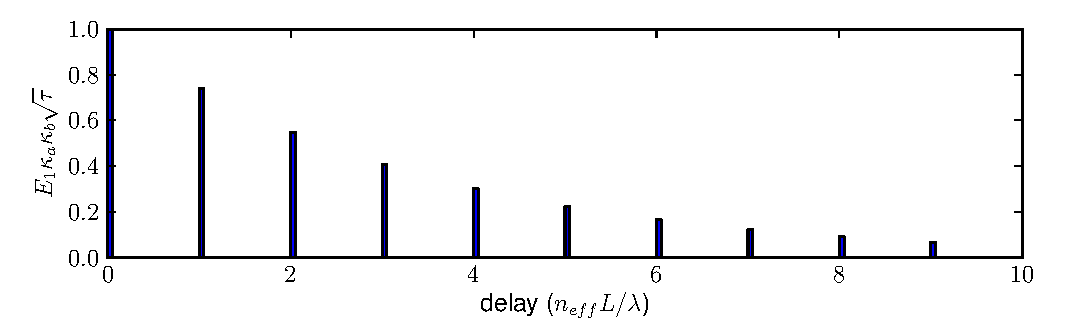
\includegraphics{exp_decay}
\caption{\label{fig:exp decay}}
\end{figure}
Another important equation that can be derived from \ref{eq:drop efficiency} is the Q factor
\begin{equation}
Q=\frac{\lambda_{0}}{\Delta\lambda_{\text{FWHM}}}=\frac{\pi L_{\text{eff}}n_{g}}{\lambda_{0}\arccos\left(\frac{1-t_{a}^{2}t_{b}^{2}\tau-4t_{a}t_{b}\tau}{-2t_{a}t_{b}\tau}\right)},
\label{eq:Q}
\end{equation}
where we see that it depends mainly on the coupling between the cavity to the waveguides and the intrinsic loss.
%\footcite{Miyagi:1978p1770,Baets:1983p1772,Hutcheson:1980p1771}

\section{Material optical properties}

Geometric variation of components allows for the properties shown so far, although to guide light it was key to leverage difference in index of refraction of distinct materials. But a diversity of other material optical properties can be exploited for a variety o ends. Thermo-optic effect allows for a easy way to change materials index of refraction, despite the fact that is relatively slow. Plasma dispersion together with electron injection can be used to rapidly and electrically change the index of refraction of semiconductors. For semiconductor with bandgap smaller than the photon energy we have simple way to turn light into current.

\subsection{Material dispersion}

Material index of refraction varies with the frequency of the electromagnetic radiation propagating on it. This dispersion modifies light group velocity which are determined the resonators \gls{FSR}, and therefore, it cannot be ignored. Good estimation of materials index of refraction can be made using \fnurl{Sellmeier's empirical relation}{http://en.wikipedia.org/wiki/Sellmeier_equation}
\begin{equation}
n^{2}\left(\lambda\right)=1+\sum_{i}A_{i}\frac{\lambda^{2}}{\lambda^{2}-\lambda_{i}^{2}}.\label{eq:sellmeier equation}\end{equation}
where $\lambda$ is the vacuum wavelength is in micrometers, $A_i$ and $\lambda_i$ are the Sellmeier coefficients. The table \ref{table:silicon sellmeier coefficients} shows the Sellmeier's coefficients for Si\footcite{Tropf:1994p49} and \ce{SiO2}.
\begin{table}[H]
\noindent \begin{centering}
\begin{tabular}{ccccccccc}
\hline 
 & $\lambda_{1}$ & $\lambda_{2}$ & $\lambda_{3}$ & $A_{1}$ & $A_{2}$ & $A_{3}$ \tabularnewline
\hline
\hline 
Si & 0.301516485 & 1.13475115 & 1104.0 & 10.6684293 & 0.00304347484 & 1.54133408 \tabularnewline
\hline 
\ce{SiO2} & 0.0260605 & 0.116241 & 9.89616 & 0.6961663 & 0.4079426 & 0.8974794 &  \tabularnewline
\hline
\end{tabular}
\par\end{centering}
\caption{Sellmeier coefficients for silicon and silicon oxide.\label{table:silicon sellmeier coefficients}}
\end{table}


\subsection{Thermo optic effect}
The refractive index of optical materials is not a constant parameter over the temperature region in which the materials, such as crystals, semiconductor, and glasses are used. The variation of refractive index with the temperature at a constant pressure is called the thermo-optic coefficient. It is denoted as $dn/dT$, where $n$ and $T$ are the refractive index and temperature, respectively. Its unit is per degree centigrade or Kelvin. In comparing with silica, silicon has a relatively high thermo-optic coefficient of $\partial n/\partial T=\left(1.86\pm0.08\right)\times10^{-4}\text{K}^{-1}$\footcite{Cocorullo:1992p1595}. Although this property is hurdle for in the stability of electro optic silicon modulator, it is also a convenient way to tune the refractive index.

%\section{Conclusion}


%\subsection{Electro-optic effect}
%
%
%\subsection{Effect $\chi^{3}$}
%
%%
%\begin{table}[H]
%\noindent \begin{centering}
%\begin{tabular}{cccc}
%\hline 
% & & $\lambda=1.54\text{\ensuremath{\mu}m}$ & \tabularnewline
%\cline{2-4} 
%Material & $n_{2}\left(\text{cm}^{2}/\text{W}\right)$ & $\beta\left(\text{cm}/\text{GW}\right)$ & $F$\tabularnewline
%\hline
%\hline 
%Si $\left\langle 110\right\rangle $ & $0.45\times10^{-13}$ & 0.79 & 0.37\tabularnewline
%Si $\left\langle 111\right\rangle $ & $0.43\times10^{-13}$ & 0.88 & 0.32\tabularnewline
%GaAs & $1.59\times10^{-13}$ & 10.2 & 0.10\tabularnewline
%\hline
%\end{tabular}\ \begin{tabular}{ccc}
%\hline 
% & $\lambda=1.27\text{\ensuremath{\mu}m}$ & \tabularnewline
%\hline 
%$n_{2}\left(\text{cm}^{2}/\text{W}\right)$ & $\beta\left(\text{cm}/\text{GW}\right)$ & $F$\tabularnewline
%\hline
%\hline 
%$0.26\times10^{-13}$ & 0.74 & 0.28\tabularnewline
%N/A & N/A & N/A\tabularnewline
%$-0.79\times10^{-13}$ & 15.1 & 0.004\tabularnewline
%\hline
%\end{tabular}
%\par\end{centering}
%
%\caption{Measured two-photon absorption and Kerr coefficients for silicon and
%gallium arsenide. The relative errors are estimated as $\pm15\%$.\footcite{Dinu:2003p1592}}
%
%\end{table}
%
%
%\subsection{Plasma dispersion}
%%
%\begin{figure}[H]
%\input{silicon_electrorefraction.pdf_tex}
%%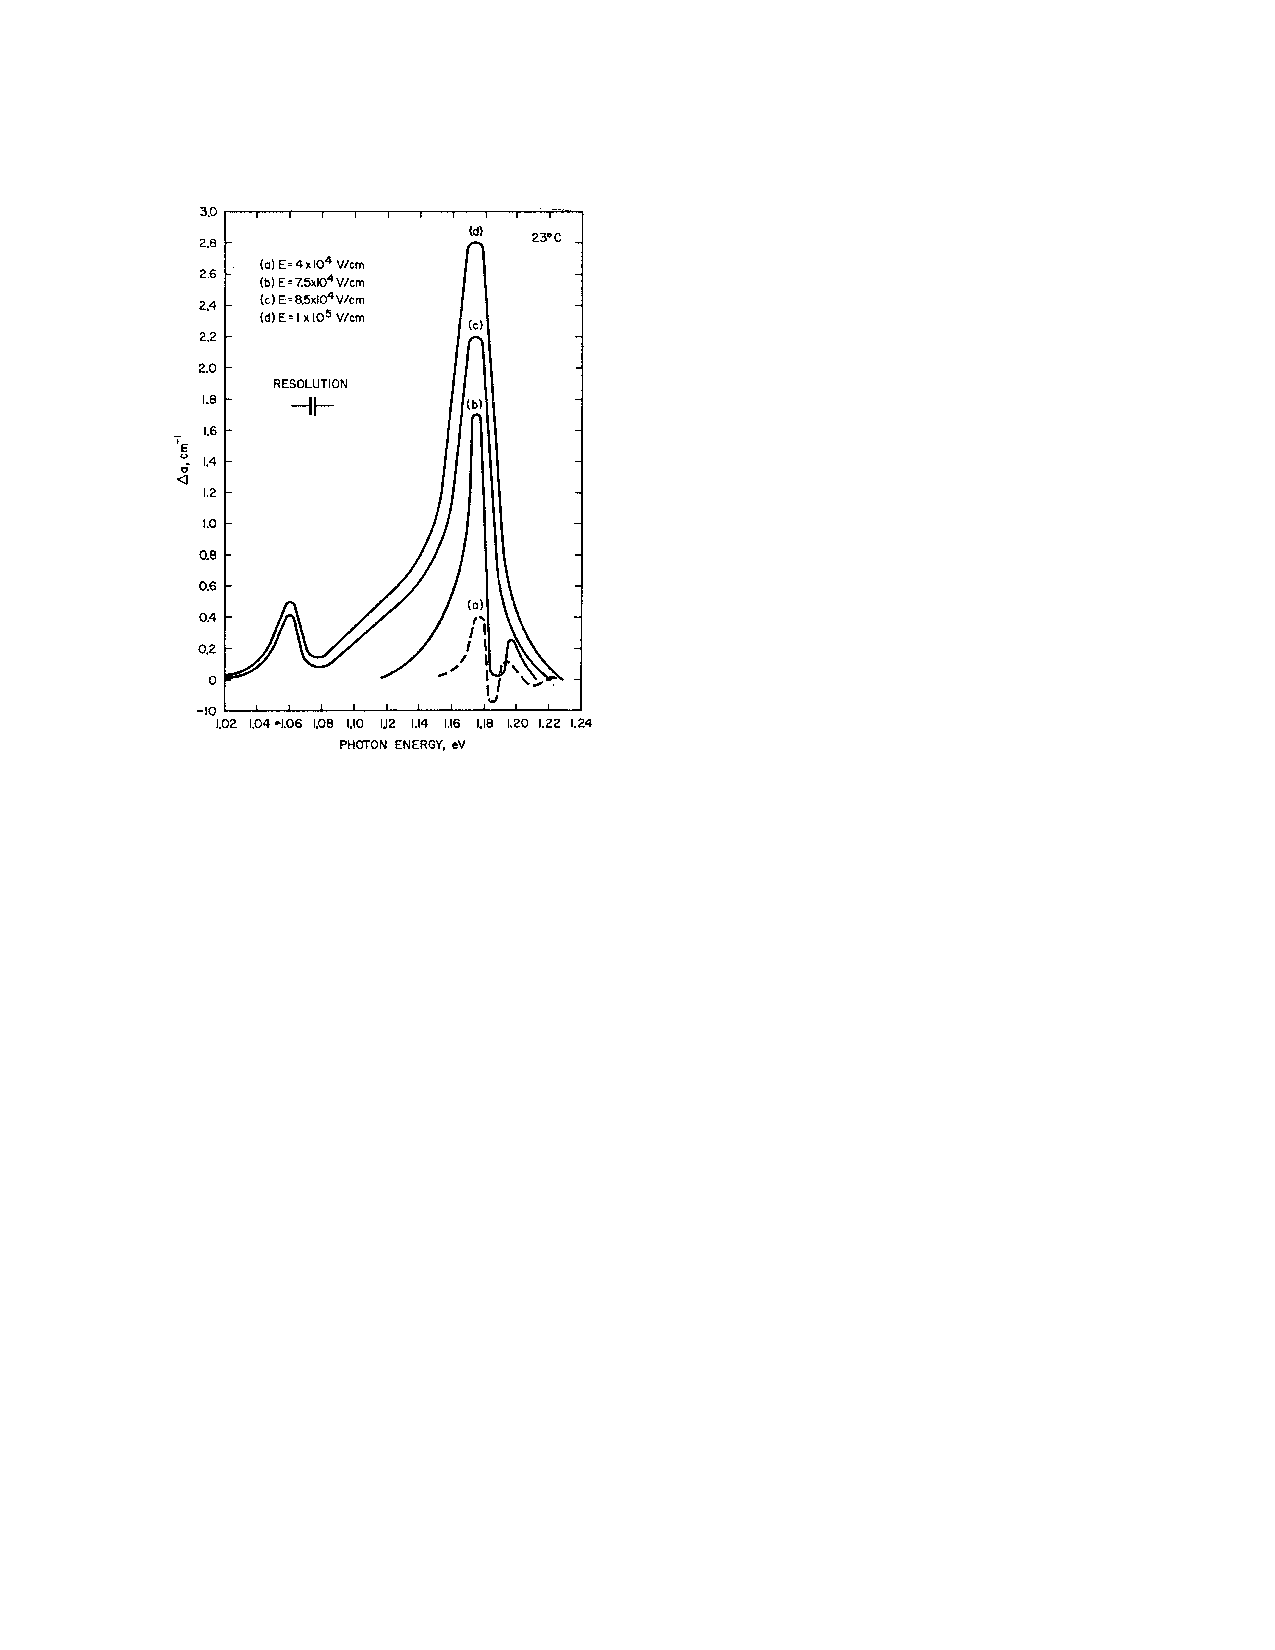
\includegraphics{/Users/bernardo/Dropbox/thesis/figures/SiElectroabsorption}
%\caption{(a) Electro-absorption and (b) electro-refraction versus wavelength in c-Si. Electro-absorption horizontal axis is linear in photon energy.\footcite{Soref:1987p1492}}
%\end{figure}
%\section{Light Source and Detectors}
%To conclude the chapter we shall discuss a little of the conversion between electricity and light. 
%\fnurl{Superlum}{http://www.superlumdiodes.com}
%
%Detector are the converter from photonics to electronics. As with light sources the material which the detector is made of needs to be integrated to the rest of the circuit. The most used detector type relies on the excitation of electrons from the valence band to the conduction band of a semiconductor material, by the photons to be detected. But other physical effects can be used to make detector. {[}examples{]}
%
%Semiconductor detector, nevertheless, are the most used due to its bandwidth, limited by the electron mobility which allows bandwidth of {[}numbers for{]}. Sensitivity, (operating in avalanche mode single photons can be detected). Simplicity, in metal-semiconductor-metal (MSM) the only thing needed is the detecting semiconductor material and the metal contacts. Doping the endpoints of the detector creating a PIN structure will allow eliminate the need for an external voltage drive.
%
%\footcite{Assefa:2009p35}
%
%Two materials are most commonly used. Germanium and Indium Galium
%Arsenide (InGaAs)
%
%%
%\begin{figure}[h]
%\noindent \centering{}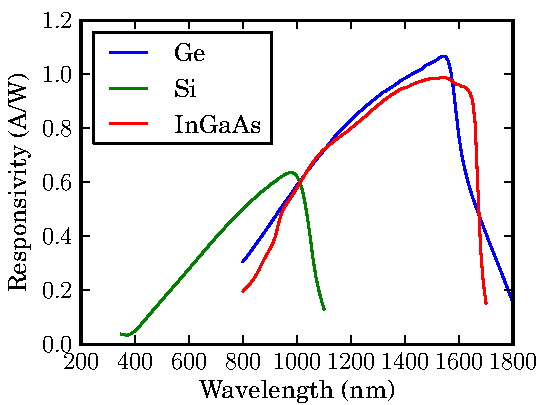
\includegraphics{graphs/detectorResponsivity}\caption{Responsivity for most used detector materials.}
%
%\end{figure}
%
\chapter{Diffraction Grating Spectrometers}
It is difficult to enumerate all the contribution to society that diffraction grating has brought. Its role on identifying the discrete energy levels of atoms provided a significant amount of information to the development of quantum mechanics. Currently its use in the identification or quantification of chemical compounds and its structure constitutes the majority usage end of diffraction gratings.

%Historically, diffraction grating spectrometers have been bulky table top devices. But sizes have been decreasing, and handheld devices are already commercialized. Further in the chapter we will discuss how the devices is limited. 

%Diffraction grating spectrometers can be integrated on chips, and this type of devices have been manufactured for wavelength de-multiplexing devices in the telecommunication industry. 


%\section{alternatives}
%
%Multi-aperture planar waveguide spectrometer formed by arrayed Mach-Zehnder interferometers\footcite{Florjanczyk:2007p1602}
%
\section{Kirchhoff's diffraction theory}

\begin{figure}
\begin{minipage}[t]{0.48\textwidth}
\input{aperture_diffraction.pdf_tex}
\caption{}
\label{fig:aperture}
\end{minipage}
\hfill
\begin{minipage}[t]{0.48\textwidth}
\input{aperture_coord.pdf_tex}
\caption{}
\label{fig:aperture coord}
\end{minipage}
\end{figure}

To establish the terminology we give a brief review of diffraction theory. Starting with Huygens principle that states that each point of a wavefront is a new wave source. With such principle in mind, the problem of the diffraction by a small aperture, depicted at figure \ref{fig:aperture}, can seen in the following way. If waves are generated by a point source $P_{0}$ at a point $Q$ the wave field should be
\begin{equation}
E\left(Q\right)=E\left(P_{0}\right)\frac{e^{ikr}}{r},
\label{}
\end{equation}
where r the distance between $P_{0}$ and $Q$, and $k$ is the wavenumber. The field at a point $P$ due to source at $Q$ is then
\begin{equation}
E\left(P\right)=E\left(P_{0}\right)\frac{e^{ikr}}{r}\frac{e^{iks}}{s}K\left(\chi\right),
\end{equation}
where $K\left(\chi\right)$ is an inclination factor which describes the variation with direction of the amplitude of the secondary waves, $\chi$ been the angle between the primary wavefront normal and the direction of $QP$. The electric field at $P$ due to all wave sources at surface $S$ will then be
\begin{equation}
E\left(P\right)=E\left(P_{0}\right)\int_{S}\frac{e^{ikr}}{r}\frac{e^{iks}}{s}K\left(\chi\right)dS.
\label{eq:huygens formula}
\end{equation}
The Huygens principle was then put on a sounder mathematical basis by Kirchhoff \footnote{Section 8.3 Born and Wolf}. Using Green's theorem on the time-independent wave equation $\left(\nabla^{2}+k^{2}\right)E=0,$ one can derive that
\begin{equation}
E\left(P\right)=\frac{1}{4\pi}\int_{S}\left[E\left(Q\right)\frac{\partial}{\partial n}\left(\frac{e^{iks}}{s}\right)-\frac{e^{iks}}{s}\frac{\partial E}{\partial n}\left(Q\right)\right]dS,
\end{equation}
where $\partial/\partial n$ is the differentiation along the normal to $S$. This one form of the integral theorem of Helmholtz and Kirchhoff. Since $\frac{\partial}{\partial n}\left(\frac{e^{iks}}{s}\right)=\frac{e^{iks}ik}{s}\left[1-\frac{1}{iks}\right]\cos\left(n,s\right)$, considering that $ks\gg1$
\begin{equation}
E\left(P\right)=\frac{1}{4\pi}\int_{S}\frac{e^{iks}}{s}\left[ikE\left(Q\right)\cos\left(n,s\right)-\frac{\partial E}{\partial n}\left(Q\right)\right]dS,
\label{eq:integral theorem}
\end{equation}

For a point source at $P_{0}$ the field at $Q$ is $E\left(Q\right)=E\left(P_{0}\right)\frac{e^{iks}}{s}$.
The Fresnel-Kirchoff formula will be
\begin{equation}
E\left(P\right)=\int_{S}E\left(P_{0}\right)\frac{-ik}{4\pi}\frac{e^{ikr}}{r}\frac{e^{iks}}{s}\left[\cos\left(n,r\right)-\cos\left(n,s\right)\right]dS,
\label{eq:Fresnel-Kirchhoff}
\end{equation}
which is known as the Fresnel-Kirchhoff diffraction formula. Since $\cos\left(n,r\right)=1$ and $\left(n,s\right)=\pi-\chi$ the above integral is
\begin{equation}
E\left(P\right)=E\left(P_{0}\right)\int_{S}\frac{e^{ikr}}{r}\frac{e^{iks}}{s}\frac{-ik}{4\pi}\left(1+\cos\chi\right)dS.
\end{equation}

This validates the Huygens principle. Comparing with \ref{eq:huygens formula} we note that
\begin{equation}
K\left(\chi\right)=\frac{-ik}{4\pi}\left(1+\cos\chi\right).
\end{equation}


A special case of the Fresnel-Kirchhoff diffraction formula is the Fraunhofer diffraction, in this case, the diffracting element is much smaller than the distances where the field is being evaluated. Figure \ref{fig:aperture coord}, depict such case. Where the assumption is that $\frac{W}{r}$ and $\frac{W}{s}\ll1$. In such case we have that
\begin{equation}
s'\approx s+\xi\sin\theta
\end{equation}
\begin{equation}
r'\approx r+\xi\sin\theta_{0}
\end{equation}


which will cause the Fresnel-Kirchhoff formula to be approximated to
\begin{equation}
E\left(P\right)=C\int_{-W/2}^{W/2}e^{ik\xi\left(\sin\theta_{0}+\sin\theta\right)}d\xi,
\label{eq:Fraunhofer}
\end{equation}
where $C=E\left(P_{0}\right)\frac{-ik}{4\pi}\frac{e^{ikr}}{r}\frac{e^{iks}}{s}\left(\cos\theta-\cos\theta_{0}\right)$
\begin{equation}
E_{\text{aperture}}=CW\text{sinc}\left[\left(\sin\theta_{0}+\sin\theta\right)\frac{Wk}{2\pi}\right].
\end{equation}

\section{Diffraction grating}
\label{section:Diffraction-grating}
A diffraction grating may be defined as any arrangement which imposes on an incident wave a periodic variation of amplitude, phase, or both.
Let us now consider a one-dimensional grating consisting of $N$ parallel apertures on one surface. Let the $\xi$-plane coincide with the plane face of the plate, and let $d$ be the period in the $\xi$ direction. As shown in figure \ref{fig:grating ex}. Assume that the direction of propagation of the wave incident upon the grating is in the plane of the figure, making an angle $\theta_{0}$ with $O\zeta$, and let $\theta$ denote the angle which $O\zeta$ makes with the line joining a very distant point of observation $P$ with the grating.

\begin{figure}[h]
\center{\input{grating-ex.pdf_tex}}
\caption{Diffraction grating cross section.}
\label{fig:grating ex}
\end{figure}
Fraunhofer aperture formula \ref{eq:Fraunhofer} can be analogously used to calculate the field at $P$
\begin{equation}
E\left(P\right)=C\sum_{n=0}^{N}\int_{nd-W/2}^{nd+W/2}e^{ik\xi\left(\sin\theta_{0}+\sin\theta\right)}d\xi,
\end{equation}
making the change of variable $\xi=\xi'-nd$, taking out of the integral all terms factors that don't depend on $\xi'$ we arrive at
\begin{equation}
E_{\text{grating}}=E_{\text{aperture}}\sum_{n=0}^{N}e^{-iknd\left(\sin\theta_{0}+\sin\theta\right)},
\label{eq:Up}
\end{equation}
Hence 
\begin{equation}
I\left(p\right)=\left|E\left(p\right)\right|^{2}=I_{\text{aperture}}\frac{1-\cos Nkdp}{1-\cos kdp}
\label{eq:Ip grating}
\end{equation}
where $I\left(p\right)=\left|E\left(p\right)\right|^{2}$ and $p=\sin\theta_{0}+\sin\theta$. If we introduce the function
\begin{equation}
H\left(N,x\right)=\left(\frac{\sin Nx}{\sin x}\right)^{2},
\end{equation}
the formula \ref{eq:Ip grating} for the intensity may be written as
\begin{equation}
I\left(p\right)=H\left(N,\frac{kdp}{2}\right)I_{\text{aperture}}.
\label{eq:intensity grating}
\end{equation}
Before discussing the implications of this formula we note that according to \ref{eq:Up}, the light distribution is the same as that due to a set of coherent secondary sources each characterized by the same amplitude function $\left|E^{\left(0\right)}\left(p\right)\right|$ and with phases that differ form each other by integral multiples of $kdp$. To see the significance of this phase difference consider two corresponding points $A$ and $B$ in the neighboring grooves of the grating (Fig. \ref{fig:grating ray}). Since the effect of the grating is to impress a periodic variation onto the incident wave, it follows that the path difference between the light arriving a $A$ and at $B$ is the same as in the absence of the grating, i.e. it is equal to $AK=d\sin\theta_{0}$, $K$ denoting the foot of the perpendicular from $B$ on to the ray incident at $A$. Further, the light path from $B$ in the direction $\theta$ exceeds the light path from $A$ by $BL=d\sin\theta$, $L$ being the foot of the perpendicular from $A$ on to the ray diffracted at $B$ in the direction $\theta.$ Hence the total path difference between light arriving at the distant point of observation form corresponding points in two neighboring grooves is
\begin{equation}
BL-AK=d\left(\sin\theta-\sin\theta_{0}\right)=dp,
\label{eq:path difference}
\end{equation}
 and the corresponding phase difference is $2\pi dp/\lambda=kdp$.

\begin{figure}
\begin{minipage}[t]{0.48\textwidth}
\input{grating-ray.pdf_tex}
\caption{Illustrating the theory of diffraction grating.}
\label{fig:grating ray}
\end{minipage}
\hfill
\begin{minipage}[t]{0.48\textwidth}
%\input{aperture_coord.pdf_tex}
\caption{}
\label{fig:aperture coord}
\end{minipage}
\end{figure}

Formula \ref{eq:intensity grating} expresses $I\left(p\right)$ as the product of two functions: one of them, $I_{\text{aperture}}$, represents the effect of a single period of the grating; the other, $H$, represents the effect of the interference of the light from different periods. The function $H\left(N,x\right)$ has maxima, each of height $N^{2}$, at all points where the denominator $\sin^2 x$ vanishes. Hence $H\left(N,kdp/2\right)$ has maxima of height $N^2$ when
\begin{equation}
p\equiv\sin\theta-\sin\theta_{0}=\frac{m\lambda}{Nd}\left(m=0,\pm1,\pm2,\ldots\right),
\label{eq:grating equation}
\end{equation}
The integer $m$ represents, according to \ref{eq:path difference}, the path difference in wavelengths between light diffracted in the direction of the maximum, from corresponding points in two neighboring grooves. We call $m$ the \emph{order of interference}. Between theses principal maxima there are weak secondary maxima (see figure \ref{fig:diff graphs}), the first secondary maximum being only a few percent of the principal maximum when $N$ is large. The maxima are separated by points of zero intensity at $x=kdp/2=\pm n\pi/N$, i.e. in directions given by\begin{equation}
p\equiv\sin\theta-\sin\theta_{0}=\frac{n\lambda}{Nd}\left(n=0,\pm1,\pm2,\ldots\right)\label{eq: grating secondary maxima}\end{equation}
the case where $n/N$ is an integer being excluded.



%As before we set $l_{o}=\sin\theta_{0}$, $l=\sin\theta$, $p=l-l_{0}=\sin\theta-\sin\theta_{0}$. The complex amplitude at $P$ is then immediately obtained from, where the integrand must be multiplied by the transmission function $F$ of one periodic element. We may set $q=0$ and\begin{equation}
%\begin{array}{ccc}
%\xi_{n}=nd, & \eta_{n}=0 & \left(n=0,1,\ldots,N-1\right)\end{array}.\end{equation}
%We the obtain\begin{equation}
%U\left(p\right)=U^{\left(0\right)}\left(p\right)\sum_{n=0}^{N-1}e^{-ikndp}=U^{\left(0\right)}\left(p\right)\frac{1-e^{-iNkdp}}{1-e^{-kdp}},\label{eq:Up}\end{equation}
%where\begin{equation}
%U^{\left(0\right)}\left(p\right)=C\int_{A}\! F\left(\xi\right)e^{-ikp\xi}\, d\xi.\label{eq: diffraction envelope}\end{equation}
%Hence\begin{equation}
%I\left(p\right)=\left|U\left(p\right)\right|^{2}=\frac{\left(1-e^{-Nkdp}\right)}{\left(1-e^{-kdp}\right)}\cdot\frac{\left(1-e^{Nkdp}\right)}{\left(1-e^{kdp}\right)}\left|U^{\left(0\right)}\left(p\right)\right|^{2}=\frac{1-\cos Nkdp}{1-\cos kdp}I^{\left(0\right)}\left(p\right),\end{equation}

The function $I_{\text{aperture}}$ depends on the form of the period. Suppose that it has principal maximum for some direction $p=p'$ and that on both sides of the maximum it falls off slowly in comparison with $H$. Then $I\left(p\right)$ will have the general form of the interference function $H$, but will be 'modulated' by $I_{\text{aperture}}$. Thus $I\left(p\right)$ will still have a sharp maxima near the directions $p=m\lambda/d$. Since these directions (except for $m=0$) depend on the wavelength, we see that the grating will decompose a beam of non-monochromatic light into \emph{spectral orders}.

%To illustrate these remarks let us consider a grating consisting of a succession of long equidistant slits, each of width $s$ and length $L$, in an opaque screen. If the grating is illuminated from a very distant line source parallel to the slits, the intensity $I^{\left(0\right)}$ is given by the expression \ref{eq: diffraction envelope} (with $2a=s$, $2b=L$) and we obtain\begin{equation}
%I\left(p\right)=\frac{sE}{\lambda R^{2}}\left(\frac{\sin\frac{Nkdp}{2}}{\sin\frac{kdp}{2}}\right)^{2}\left(\frac{\sin\frac{kdp}{2}}{\frac{kdp}{2}}\right)^{2}.\label{eq: diffraction intensity}\end{equation}
%Curves representing the two factors in \ref{eq: diffraction intensity} and their product are shown in fig X. The last factor in \ref{eq: diffraction intensity}, which represents the effect of a single slit, has a principal maximum at $p=0$ and minima given by $ksp/2=n\pi$, i.e. at\begin{equation}
%p=\frac{n\lambda}{s},\left(n=0,\pm1,\pm2,\ldots\right)\end{equation}
% separated by weak secondary maxima. We see that if $\lambda/s\gg\lambda/d$, i.e. if the width of each slit is small compared to $d$, the intensity $I\left(p\right)$ has in addition to a principal maximum at $p=0$ a series of sharp, but progressively decreasing, maxima on either side of it, near direction given by \ref{eq:grating equation}.

It is evident that if the width of each aperture is very small, of the order of a wavelength (as is often the case in practice) the formula derived on the basis of Kirchhoff's approximation, can evidently no longer be expected to hold. In such cases more refined considerations must be make to determine the detailed distribution of the intensity. We may, however, expect that the main qualitative features indicated by our elementary theory, namely the existence of sharp maxima whose positions are substantially determined by the interference function $H$, remain even when the grooves are very narrow, provided, that the intensity function of a single period varies slowly in an interval of the order $\Delta p=\lambda/d$. Let us now consider the resolution that may be attained with a grating. The separation between a primary maximum of order $m$ and a neighboring minimum is, according to \ref{eq: grating secondary maxima}, given by
\begin{equation}
\Delta p=\frac{\lambda}{Nd}.
\end{equation}
If the wavelength is changed by an amount $\Delta\lambda$, the $m$th-order maximum is according to \ref{eq:grating equation}, displaced by an amount
\begin{equation}
\Delta'p=\frac{\left|m\right|}{d}\Delta\lambda.
\end{equation}
Assuming that the lines of wavelength $\lambda\pm\frac{1}{2}\Delta\lambda$ will just be resolved when the maximum of the one wavelength coincides with the first minimum of the other we have on he limit of resolution in the $m$th order, $\Delta p=\Delta'p$, i.e.
\begin{equation}
\frac{\lambda}{\Delta\lambda}=\left|m\right|N.
\label{eq:resolving power}
\end{equation}
Thus, \emph{the resolving power is equal to the product of the order number $m$ and the number $N$ of the grooves}. For the $m$th order we have, according to, that $d\left(\sin\theta-\sin\theta_{0}\right)=m\lambda$, so that we may also express the resolving power in the form
\begin{equation}
\frac{\lambda}{\Delta\lambda}=\frac{Nd\left|\sin\theta-\sin\theta_{0}\right|}{\lambda}.
\end{equation}
Because of \ref{eq: path difference} this implies that \emph{the resolving power is equal to the number of wavelengths in the path difference between rays that are diffracted in the direction $\theta$ from the two extreme ends (separated by distance Nd) of the grating}.
It is to be noted that since $\left|\sin\theta-\sin\theta_{0}\right|$ cannot exceed 2, the resolving power that can be attained with a grating of overall with $w$ can never exceed the value $2w/\lambda$.

\begin{figure}[H]
\center{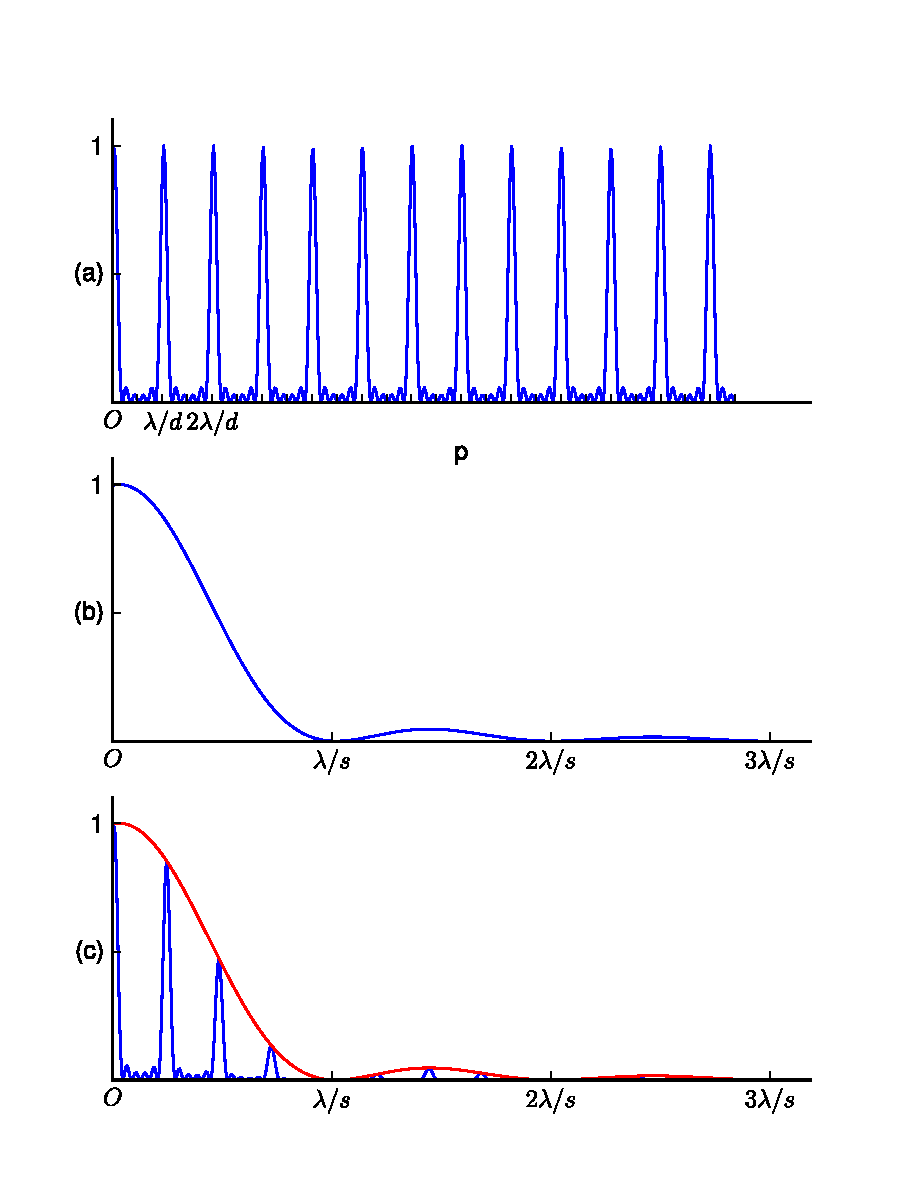
\includegraphics[scale=0.9]{diffraction-grating-basic.pdf}}\caption{}
\label{fig:diff graphs}
\end{figure}

%
%(a) The normalized interference function\begin{equation}
%\frac{1}{N^{2}}H\left(N,kdp/2\right)=\left[\frac{\sin\left(Nkdp/2\right)}{N\sin\left(kdp/2\right)}\right]^{2}.\end{equation}
%(b) The normalized intensity function of a slit\begin{equation}
%I^{\left(0\right)}\left(p\right)=\left[\frac{\sin ksp/2}{ksp/2}\right]^{2}.\end{equation}
%(c) The normalized intensity function of a grating consisting of $N$
%similar equidistant parallel slits\begin{equation}
%\frac{1}{N^{2}}I\left(p\right)=\left[\frac{\sin\left(Nkdp/2\right)}{N\sin\left(kdp/2\right)}\right]^{2}\left[\frac{\sin ksp/2}{ksp/2}\right]^{2}.\end{equation}
%Only the range $p\ge0$ is shown, all the curves being symmetrical
%about the vertical axis $p=0$.

\subsection{Free spectral range}

From the resolving power equation \ref{eq:resolving power}, we conclude that spectrometer should be operated on high diffraction order so as to minimize the device size for a given resolution. Unfortunately, from the grating equation \ref{eq:grating equation}, $p\equiv\sin\theta-\sin\theta_{0}=\frac{m\lambda}{Nd}$, we see that it is possible for light from to different wavelength in different diffraction orders to be diffracted to the same angle $\theta$, sufficing that 
\begin{equation}
m_{i}\lambda_{i}=m_{j}\lambda_{j}
\end{equation}
for $i\neq j$, so for example light diffracted in order 1 at wavelength 1500 nm is diffracted in the same direction as light diffracted from order 2 wavelength 750 nm. To avoid this ambiguity, it is of interest to know when this condition happens. From the grating equation we see that $p$ does not make sense outside the interval {[}0,1{]}, therefore, $0\le\frac{m\lambda_{m}}{Nd}\le1$ we then find that for the diffraction order $m$ the wavelength range that is going to be diffracted is:
\begin{equation}
0\le\lambda_{m}\le\frac{Nd}{m}.
\end{equation}
So for the first order the wavelength range that exists is every wavelength below $Nd$ , for order 2 every wavelength below $Nd/2$ and so on. We see then, that for order 1 the range $[Nd,Nd/2]$ is occupied solely by order one. For order 2 the range $[Nd/2,Nd/3]$, for order $m$, $[Nd/m,Nd/(m+1)]$. We see that the range width $\Delta\lambda_{m}$
which there is no overlapping diffraction, called \emph{free spectral range}, can be computed as
\begin{equation} 
\Delta\lambda_{m}=\frac{Nd}{m}-\frac{Nd}{m+1}=\frac{Nd}{m(m+1)},
\end{equation}
we can replace the dependence on $Nd$ for the wavelength in the center of the free spectral range $\lambda_{Cm}$,
\begin{equation}
\lambda_{Cm}=\frac{Nd}{m}-\frac{\Delta\lambda_{m}}{2}=\frac{Nd}{m(m+1)}(m+0.5),
\end{equation}
It is worth noting that although $\lambda_{Cm}$ is in the middle of the spectral range $\Delta\lambda_{m}$ the wavelengths are not linearly distributed along the angle range that it is diffracted to, and therefore $\lambda_{Cm}$ is not located at the center of the angle range of the $m$th order free spectral range. We see then that the free spectral range depends inversely with the diffraction order used,
\begin{equation}
\Delta\lambda_{m}=\frac{\lambda_{Cm}}{m+0.5}.
\label{eq:FSR}
\end{equation}
This fact, ties to use a maximum operating diffraction order to the wavelength range and central wavelength we want the diffraction grating to operate.

\section{Planar devices}

The previous exposition on diffraction grating does not change on the medium in which the device is built on. But since we are interested in spectrometer integrated on chips, it is worth highlighting the characteristics of this device. From this point two features stand out as very different from regular free space spectrometer. First is that light is always guided in a slab waveguide, the confinement of light in one dimension change the nature of the system from a three dimensional to bi-dimensional one, and this fact causes the light power to decay with the inverse of the distance as it moves away from the source. The other difference is the change of the dispersion due to both the material and the confinement effect. The outcome of this is that for all the results in the previous section, the wavelength variable that needs to be considered is the effective wavelength in the medium.
\begin{equation}
\lambda_{\text{eff}}=\frac{\lambda}{n_{\text{eff}}}\end{equation}
\section{Spectrometer architectures}

Several architectures to build diffraction grating spectrometer exist. Due to lowest $\text{size}\times \text{resolution}$ of the Rowland design, it was chosen to build the spectrometer. The Czerny-Turner is presented here to introduce spectrometer because its design is easily understandable. Arrayed waveguide grating has been the most used planar (on chip) version of spectrometer. Marketed as \gls{WDM} in the telecommunication sector, this layout is shown because to understand why it is not fit for the role as a high resolution on chip spectrometer. 

\subsection{Czerny-Turner}
\label{sub:Czerny-Turner}

Due to its modularity this architecture is probably the best to introduce spectrometers. It is composed of two slits, two concave mirrors and a diffraction grating. As shown in figure \ref{fig:Czerny-Turner-architecture}, the light to be analyzed is shone through the entrance slit. Due to diffraction, the light fans out as it propagates to the collimating concave mirror where light is collimated and reflected in the direction of the diffraction grating. The diffraction grating then, deviates light from each different wavelength (optical frequencies) into different angles following the equation \ref{eq:grating equation}. A focusing concave mirror focus the light coming from the diffraction grating and deflects it to the detector slit.

%
\begin{figure}[h]
\centering\input{czerny-turner.pdf_tex}
\caption{Czerny-Turner architecture.}
\label{fig:Czerny-Turner-architecture}
\end{figure}

The function of the entrance slit is to filter spatial optical modes that are inputed into the system. For best filtering the slit has to transmit only a single spatial mode. This is achieved by making the slit width of the order of the light wavelength. Decreasing slit width will increase the beam spread angle, as depicted in figure \ref{fig:different slits}, for a chosen final beam width this will allow the collimating concave mirror to be placed nearer to the slit decreasing the device size. However, reducing the slit width will also decrease the fraction of transmitted light. and therefore, lowering the device sensitivity.

%
\begin{figure}[h]
\centering
\input{slit_width.pdf_tex}
\caption{Different effects of slit width.}
\label{fig:different slits}
\end{figure}

As described by its name the collimating concave mirror collimates the light coming from the entrance mirror and redirects it to the diffraction grating. In order to \fnurl{collimate}{http://en.wikipedia.org/wiki/Collimated_light} the input light, the curvature radius should be equal twice the distance from the entrance slit to the center of the collimating concave mirror. The mirror diameter must be bigger than the beam width the when it arrives at it to avoid light leakage through the mirror edges.

The diffraction grating deviates light from each different wavelength into different angles, as described by equation \ref{eq:grating equation}. Details on how the light is diffracted are explained in section \ref{section:Diffraction-grating}. Roughly, the number of illuminated grooves, which is equal to the beam diameter divided by the groove pitch, will determine the resolving power of the spectrometer, as shown in equation \ref{eq:resolving power}.

To quantify the amount of light deviated to each different direction, we use a focusing concave mirror, which will map light with different direction and focus them each into a distinct point in a plane. Clearly, the size of the focusing mirror must be such that it collects most of the light coming from the diffraction grating. This means that it must be bigger than the beam size and account the spread of different wavelengths.

A detector is placed at a point in the focus plan to measure the light power. Optimum detector size is of the order of the entrance slit width, limited also by the resolving power of the diffraction grating. Placing a exit slit in the focus plane followed by a detector, can be used as an alternative for the slit size detector. 

\subsection{Rowland\label{sub:Rowland}}

In year, Rowland \footcite{Rowland:1883p38} found a way to incorporate the collimating and focusing elements into the diffraction grating. This layout not only decreased the final device size, but also eliminate spherical and astigmatism aberrations due to the auxiliary concave mirrors.

The design consists in the use of a concave diffraction grating of radius 2R. The entrance and exit slits positions are located in a circle of radius R tangent to the diffraction grating sphere. Or more precisely tangent to one of the equator of the diffraction grating sphere. For optimum area usage, the equator should be perpendicular to the diffraction grating grooves and passing through the grating center.

%
\begin{figure}[h]
\center{\input{rowland-mounting.pdf_tex}}
\caption{Rowland design.}
\end{figure}



\subsection{Arrayed Waveguide Grating (AWG)}

The resolving power of a diffraction grating is proportional to the number of grooves and diffraction order, as shown in equation \ref{eq:resolving power}. Diffraction grating based on ruled surfaces can not achieve diffraction order greater than 20. Introduced by Takahashi et. al.\footcite{Takahashi:1990p122}, this limitation can be overcome by replacing the grating grooves by an array of waveguides. To understand how the introduction of waveguide help it is necessary to understand more generally what diffraction order is. We say that certain diffraction peak is of order $m$ if each wave from the set that was constructively interfered to form the interference peak is delayed from one another of $m$ periods. On traditional ruled surface diffraction gratings, wavefront from different period are made to interfere by making the wave travel different path lengths by taking path that deviates from the equal angle reflection.

%
\begin{figure}[h]
\center{\input{awg.pdf_tex}}
\caption{Arrayed waveguide grating schematics. Notice that each waveguide has a different path-length.\label{fig:awg}}

\end{figure}
By guiding light through waveguide it is possible to increase the difference of path length among different waveguides, achieved by only changing the waveguides lengths. Each waveguide of the waveguide array would function like a groove in the diffraction grating, but since waveguide length is only limited by its intrinsic loss, the difference of path length can be on the order of hundreds of wavelength, giving raise to grating that operate of diffraction order of also hundreds.

Unfortunately there is a drawback of increasing diffraction order, the free spectral range as described in \ref{eq:FSR}, decreases with the inverse of the of the diffraction order. For instance, an arrayed waveguide grating working on diffraction order 100 at wavelength 1500 nm would have a FSR of only 15 nm. Although this range is useful for fiber optics telecommunications, this bandwidth is too small for most spectroscopy application, optical coherence tomography or ultra-fast oscilloscope\footcite{Foster:2008p71}. Since we want to achieve a wide spectrum range, this architecture is not fit for us.

\section{Grating illuminated by a gaussian beam}
\label{section:Grating gaussian beam}

%
\begin{figure}[h]
\centering\input{gaussian-beam.pdf_tex}
\caption{Diffraction grating illuminated by a (a) uniform intensity beam, (b) Gaussian beam.\label{fig:square-gaussian}} 
\end{figure}

In section \ref{section:Diffraction-grating}, it was assumed that the whole grating was uniformly illuminated. In practice, this case not always occurs. Light source is normally a collimated light from a slit, pin hole or fiber optics, where for best resolution, single mode output should pass through. In those cases the transversal power profile is better modeled by a Gaussian than by a square profile, see figure \ref{fig:square-gaussian}. To adjust the resolving power equation \ref{eq:resolving power} to account for the Gaussian profile illumination we have to alter the squared illumination assumption in equation \ref{eq:Up}. Using the relation we can equate 
\begin{equation}
E\left(p\right)=E_{\text{aperture}}\left(p\right)\int\sum_{n=-\infty}^{\infty}\delta\left(x-n\right)\text{rect}\left[\frac{x}{2\left(N-1\right)}\right]e^{-ikxdp}dx\end{equation}
where
\begin{equation}
\text{rect}\left(x\right)=\begin{cases}
0 & \mbox{if }\left|x\right|>\frac{1}{2}\\
\frac{1}{2} & \mbox{if }\left|x\right|=\frac{1}{2}\\
1 & \mbox{if }\left|x\right|<\frac{1}{2}.\end{cases}\end{equation}
the rect$\left(x\right)$ function correspond to the squared illumination assumption, for a Gaussian illumination we simply replace the function by a Gaussian function
\begin{equation}
\text{gauss}\mbox{\ensuremath{\left(x\right)}}=\exp\left[-4\ln2\left(\frac{x}{w/d}\right)^{2}\right]\end{equation}
where $d$ is the grating pitch, and $w$ is the Full Width at Half Maximum field amplitude of the illuminating beam at the grating. Replacing the Dirac delta comb by its Fourier series 
\begin{equation}
\sum_{k=-\infty}^{\infty}\delta\left(x-k\right)=\sum_{m=-\infty}^{\infty}e^{i2\pi mx},\end{equation}
we get
\begin{equation}
E\left(p\right)=E_{\text{aperture}}\left(p\right)\sum_{m=-\infty}^{\infty}\int\exp\left[-4\ln2\left(\frac{x}{w/d}\right)^{2}\right]e^{-i2\pi x\left(kdp/2\pi-m\right)}dx\end{equation}
performing the integral we obtain a comb of Gaussian 
\begin{equation}
E\left(p\right)=E_{\text{aperture}}\left(p\right)\frac{w}{\sqrt{2}}\sum_{m=-\infty}^{\infty}\exp\left[-\frac{1}{4}\left(\frac{kdp}{2\pi}-m\right)^{2}\frac{\left(w/d\right)^{2}}{4\ln2}\right],\label{eq:gaussian comb}\end{equation}
where each Gaussian is centered on the diffraction order $m$. From it we get
\begin{equation}
\frac{kdp}{2\pi}=m\mbox{ or }p=\frac{\lambda m}{d}.\label{eq:grating equation 2}
\end{equation}
From equation \ref{eq:gaussian comb} we can define the wavelength width $\Delta\lambda$ such that the power of wavelength $\lambda$ at diffraction order $m$, is halven as a been
\begin{equation}
\Delta p=2\ln2\frac{\lambda}{w},
\end{equation}
or using the grating equation \ref{eq:grating equation 2} e define the resolving power for a Gaussian beam illuminated diffraction grating as
\begin{equation}
\frac{\lambda}{\Delta\lambda}=4\sqrt{2}\ln2\frac{wm}{d}\label{eq:resolving power gaussian}\end{equation}
It is worth noting that the relationship between the electric field amplitude \gls{FWHM} $w$ at the grating and the power \gls{FWHM} $W$ is
\begin{equation}
W=\frac{w}{\sqrt{2}}
\end{equation}
Therefore
\begin{equation}
\frac{\lambda}{\Delta\lambda}=8\ln2\frac{Wm}{d}.
\end{equation}
%\section{Size}
%
%For a given wavelength $\lambda$, resolution $\Delta\lambda$ and free spectral range $\delta\lambda$, one would like to minimize the device size. Since the device size is basically defined by the grating size $W$. We have $W=a\frac{\lambda^{2}}{\Delta\lambda}$. Since $Nm=\frac{\lambda}{\Delta\lambda}$. $W=a\frac{\lambda m}{\Delta\lambda}d$, $\delta\lambda=\frac{\lambda}{m}$. $W=a\frac{\lambda^{2}}{\delta\lambda\Delta\lambda}d$

\section{Aberrations}
The resolving power equation \ref{eq:resolving power} states that the resolution of a diffraction grating depends linearly with the wavelength. Unfortunately, that relation is only valid for plane waves. To use segregation capability of the diffraction grating, it is necessary to have a source of plane waves and to measure the light power that goes to different direction after diffraction from the grating. Sources and detector are space localized at endpoints. But employing lenses, it is possible to convert a space localized mode to an angle localized mode, as discussed on the Czerny-Turner configuration in section \ref{sub:Czerny-Turner}. This conversion, however, is not perfect. In geometrical optics terms, this means that rays that enter parallel in a lens (or any other focusing device) does no converge to a single point after the lens and with the phase arriving at exactly the same time. Integrating the lens into the grating, as done in Rowland configuration in section \ref{sub:Rowland}, does not readily eliminate the problem, but its application together with the potential to fabricate designs with freedom to choose any geometry and dispersion might be the solution.

First we will state formally what conditions need to be satisfied in the design of a aberration free spectrometer. The non-existence of a mathematical solution, lead us to show two corrections, named one point and two point stigmatic correction, that reduce aberrations. 

\subsection{Aberration free conditions}
One would like to design a perfect aberration free spectrometer. The ability of electron beam lithography to define with accuracy of nanometers the position and shape of the grating grooves.

%
\begin{figure}
\centering\input{aberration-free.pdf_tex}
\caption{Diffraction grating spectrometer point problem sketch.}
\label{fig:aberration free}
\end{figure}

The problem can be stated as follows: Light coming from a point $I$ fan out to a diffraction grating which the i-th groove, of $N$ grooves, is located at $G_{i}$, at each groove light is reflected, fans out again and propagates to a set of $M$ output waveguides which the j-ith waveguide is located at $O_{j}$, as shown in figure \ref{fig:aberration free}. To perfectly separate light from different wavelengths, we would like that all light which has wavelength $\lambda_{j}$ coming from each groove arrive in phase at the output point $O_{j}$. Furthermore, we would like that light coming from each different groove have be in a different cycle. The previous conditions can be expressed by a system of $N\times M$ nonlinear algebraic equations with the prototype
\begin{equation}
\overline{IG_{i}}+\overline{G_{i}O_{j}}=\lambda_{j}\left(a_{j}+mi\right)\text{ for }\left(i=1,2,\dots,N\right)\text{ and }\left(j=1,2,\dots,M\right),\label{eq:spectrometer equation}\end{equation}
where $m$ is an integer number which defines the diffraction order and $a_{j}$ is a constant that states that the absolute path length does not matter, only the path length difference between light coming from different routes do. It is worth emphasizing that the path length evaluation should consider the medium refractive index, from this perspective one can interpret that light is also propagating in a non-Euclidean space.

For the case of a flat space in a plane, equation \ref{eq:spectrometer equation} can be expanded to
\begin{equation}
\sqrt{\left(I_{x}-G_{ix}\right)^{2}+\left(I_{y}-G_{iy}\right)^{2}}+\sqrt{\left(O_{jx}-G_{ix}\right)^{2}+\left(O_{jy}-G_{iy}\right)^{2}}=\lambda_{j}\left(a_{j}+mi\right),
\label{eq:spectrometer equation expanded}
\end{equation}
for $\left(i=1,2,\dots,N\right)$ and $\left(j=1,2,\dots,M\right)$. As discussed in sections \ref{section:Diffraction-grating} and \ref{section:Grating gaussian beam}, high resolution implies in the use of a high number of grooves $N$ with numbers typically achieving, thousands to millions. Number of channels $M$ is, of course, as a wish of the costumer but numbers around thousands are very typical. These implies that the set of equations \ref{eq:spectrometer equation expanded} is comprised of $M\times N$ equations with and $2N+2M+1$ variables.
%Real Nullstellensatz

Using a different approach it was shown that there was no configuration in a flat surface that has no aberration\footcite{Marz:1992p28,Beutler:1945p8,Namioka:1959p48,Velzel:1976p67}, but nothing has been shown for non-Euclidean surfaces. Fabrication of non-Euclidean surfaces have been used to demonstrate cloaking devices\footcite{Gabrielli:2009p1173}. Although it is not possible to find a solution for all equations, solving for one and two points dramatically improves aberration. 

\subsection{One point stigmatic correction}
Although no free of aberration configuration for all spectrometer channels exists, it can be easily seen the the equation system \ref{eq:spectrometer equation expanded} is solvable for $M\le2$. This means that it is possible to find a configuration where there is no aberration for up to two channels, or also known as stigmatic point.

For one stigmatic point, a degree of freedom is left undefined. We can use the freedom to choose the surface in which the diffraction grooves are going to be positioned\footcite{McGreer:1996p15}. Using the Rowland design as a basis, we show here how to place the grooves on a circle in order to have a wavelength free of aberration. 

Integrated device using two stigmatic points were also made\footcite{Horst:2009p1764,Gidon:1988p1765}. Due to the optimization it is the best configuration for integrated diffraction grating devices with small aberration.

%\section{Blazing and Groove size}

\section{Fresnel-Kirchhoff model}
\label{section:Rayleigh-Huygens-model}

Numerical calculation where carried out using a Fresnel-Kirchhoff method adapted to a bidimensional world\footcite{Brouckaert:2007p82}. The implementation was done in a Python script program, and the program is available at \fnurl{Google Code}{http://code.google.com/p/khsimulator/}. The adaptation to bidirectional field amplitude will decays as $1/\sqrt{r}$ instead of $1/r$ in the tri-dimensional case.

Figure \ref{fig:Huygens sketch} shows a sketch of the geometry of the simulated grating. The simulation was carried in two steps. First the field in the grating groove were calculated assuming that the field in the input waveguide had a cosine mode line shape. Then, the field in the output waveguide was calculated using the field on the grating computed in eh previous step. The amount of light coupled in to the output waveguide was estimated by carrying the inner product of the field in the output waveguide and the mode supported by that waveguide.

%
\begin{figure}[H]
\noindent \begin{centering}
\center{\input{KH.pdf_tex}}
\par\end{centering}
\noindent \centering\caption{Sketch of the geometry of the simulated spectrometer.\label{fig:Huygens sketch}}
\end{figure}

According to the Fresnel-Kirchhoff diffraction formula, the incident electric field $E_{\text{inc}}$ at the center points of the grating facets $\left(P'\right)$ at a distance $r_{1}$and at an angle $\alpha_{s}$
can be calculated as 
\begin{equation}
E_{\text{inc}}=\frac{1}{2}\sqrt{\frac{n_{\text{eff}}}{\lambda}}\int E_{\text{wg}}\left(y\right)\frac{e^{-jkr_{1}}}{\sqrt{r_{1}}}\left(1-\cos\alpha_{s}\right)dy\end{equation}
where $k=2\pi n_{\text{eff}}/\lambda$ is the wavenumber within the slab waveguide, and $E_{\text{wg}}$ is the electric field profile of the TE-polarized fundamental mode of the input waveguide. Similarly, the diffracted field $E_{\text{out}}$ on the collection waveguides is calculated as 
\begin{equation}
E_{\text{out}}\left(P''\right)=\eta\sqrt{\frac{n_{\text{eff}}}{\lambda}}\sum_{\text{Grating}}\int_{-D/2}^{+D/2}E_{\text{inc}}\left(y\right)\frac{e^{-jkr_{2}}}{\sqrt{r_{2}}}\frac{\left(\cos\alpha_{i}-\cos\alpha_{d}\right)}{2}dy'\end{equation}
where $\alpha_{i}$ and $\alpha_{d}$ are the incident and diffracted angles with respect to the normal of each grating facet, and $\eta$ is the reflection coefficient of the grating. This formula is simplified if we assume that the magnitude of the incident field $\left|E_{\text{inc}}\right|$ is constant over each facet and the phase of this field changes linearly along the length of the facet
\begin{equation}
E_{\text{inc}}\left(y'\right)=E_{\text{inc}}\left(y'=0\right)e^{+iky'\sin\alpha_{i}}.\end{equation}
This approximation is valid if the size of the facets is small compared with the distance to the input and if the angle of incidence $\alpha_{i}$ is small. This is the case if the blaze point $\left(O\right)$ is positioned near the input waveguide $\left(I\right)$. 

%\section{Comparisons of simulations and analytic solution}
\section{Simulation of spectral defects and aberrations using Fresnel-Kirchhoff model}
Simulation also provide us with a tool to observe the effects of some fabrication limitations, as, for example, the precision to which we can place a grating groove. Two grating conditions were simulated. First we shifted each groove of the waveguide in its facet normal direction by a random value in a range with different amplitudes. Figure \ref{fig:defect simulation} shows the transmission spectrum of a single channel for different amplitudes. Until a randomness of amplitude 100 nm the signal to noise ration is greater that 20 dB. Since e-beam lithography can deliver a patterning precision better than 100 nm then random errors should not be a problem.
\begin{figure}[h]
    \begin{minipage}[t]{0.48\textwidth}
    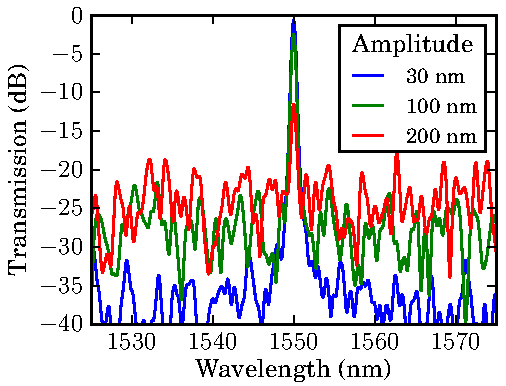
\includegraphics{random-offline-test.pdf}
    \caption{Transmission spectrum of a single channel of a grating spectrometer with the position of the grating randomly shifted. The range of possible random numbers is the amplitude.}
    \label{fig:defect simulation}
    \end{minipage}
    \hfill
    \begin{minipage}[t]{0.48\textwidth}
    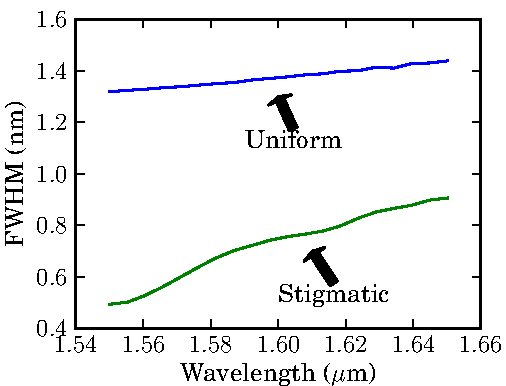
\includegraphics{graphs/aberrationComp.pdf}
    \caption{Beam waist FWHM after focusing a Diffracted on a Rowland mounting.\label{fig:stigmatic comparison graph}}
    \end{minipage}
\end{figure}

\section{Implementation}
\label{section:implementation}

%\footcite{Chowdhury:2000p56}

%The integration of silicon photonics and electronics in a CMOS compatible platform enables whole monolithic device such as a wavelength division de-multiplexer (\gls{WDM}) integrated with detectors and electronic amplifiers. Most silicon-on-insulator (SOI) \gls{WDM}s with 1 nm channel spacing typically cover a spectral range of only 10 nm. The small spectral range in typical \gls{WDM}s is due to the use of arrayed waveguide grating (AWG)\footcite{Nitkowski:2008p58,Ellis:2006p27} designs where large grating orders are employed to achieve small channel spacing which comes with the cost of free spectral range. It is possible to increase the spectral range by lowering the grating order and adding more waveguides to compensate, but this increases the overall chip size. Furthermore, due to the high index contrast of the silicon photonics platform, the achievable resolution depends on very fine control of the AWG waveguide dimensions. Here we demonstrate \gls{WDM} using etched diffraction grating (EDG)\footcite{Kneipp:1999p20,MahadevanJansen:2010p89,Foster:2008p71}.

%This design is more fabrication tolerant since light is propagating in a slab where the only dimension that needs to be controlled is the slab thickness. It is also more suitable to work at a low grating order because light diffracts in a single slab opposed to the two star couplers slabs in the AWG. 

\subsection{Design}
We designed a \gls{WDM} that uses a Rowland design with one stigmatic point correction. The system was designed so that stigmatic point was located at the central waveguide of the 21 output waveguide array. The central wavelength was chosen to be 1500 nm and the diffraction order was 10. The Rowland circle was chosen to be 750 \textgreek{m}m. The designed grating contains 340 grooves. The resulting free spectral range was estimated to be 117 nm, and the groove spacing approximately 4 \textgreek{m}m. The input and output waveguide apertures were 1.4 \textgreek{m}m. A reference waveguide was placed next to the spectrometer so that the transmission efficiency could be estimated. Unfortunately, because the TE and TM mode effective index are governed by different equations (\ref{eq:TE transcedental} and \ref{eq:TM transcedental}), the designed device is polarization sensitive. We chose to optimize the device for TE polarization.
\subsubsection{Wavelength}
Due to the readily availability of testing equipment operating at 1460-1610 nm range we decided to design the system to operate somewhere at this range. Germanium detector have a peak detection at 1500 nm so we decided to design the spectrometer operating range centered at 1500 nm.
\subsubsection{Grating size}
The spectrometer was patterned using a \fnurl{JEOL 9300FS}{http://www.jeol.com/PRODUCTS/SemiconductorEquipment/ElectronBeamLithography/JBX9300FS/tabid/152/Default.aspx} electron beam lithographer. The system is capable of writing using only beam deflection on an area (denominated \emph{field size}) of 1x1 mm. By moving the sample to be written (process called as \emph{stitching}) one is capable of writing a whole 5x5 inches mask. Unfortunately due to the extreme precision required, it is difficult to align the borders of neighboring fields perfectly, with the system working its best alignments of 10 nm are possible, though achieving this kind of precision is requires a good amount of trials and experience, alignments of 50 nm are more routinely achieved. In order to avoid errors in the spectrometer grating during stitching we limited the size of the grating in order of it to fit in a single 1x1 mm field, which meant placing the grating along the diagonal of the field, which, ignoring the grating curvature, gave us a grating size of 1.4 mm.

\subsubsection{Diffraction order}
As stated on section \ref{eq:resolving power gaussian} a higher resolving power can be achieved due to arguments to be described at X we limited our operating range to 150 nm, this would allow us to operate at diffraction order -10 or 10. 

\subsubsection{Input and output waveguides angle}
Input and output waveguides angle are defined by the compromise between the rate with which the beam sweeps across the Rowland circle as wavelength change (linear dispersion\footcite{Chowdhury:2000p56}) and space in the Rowland circle occupied by an output waveguide. From equation \ref{eq:linear dispersion} we see that it increases with decreasing input angle, and from equation \ref{eq:perimeter used} the section of the Rowland circle used by the output waveguide (perimeter used) increases with input angle. We found a good compromise with the value of input angle 35.
\begin{figure}[h]
	\begin{minipage}[t]{0.49\textwidth}
	\input{linearDispersionSchematics.pdf_tex}
	\caption{Linear dispersion schematics.\label{fig:linear dispersion}}
\end{minipage}
\hfill
\begin{minipage}[t]{0.49\textwidth}
	\input{output-shadow.pdf_tex}
	\caption{Rowland circle perimeter used by an output waveguide.\label{fig:perimeter used}}
	\end{minipage}
\end{figure}

From figure \ref{fig:linear dispersion} we see that the linear dispersion is the rate o change of output angle with the input angle $\delta\theta_{\text{out}}=\frac{\partial\theta_{\text{out}}}{\partial\lambda}\delta\lambda$ multiplied by the radius.
\begin{equation}
\text{Linear dispersion}=\frac{R}{2}\left(2\delta\theta_{\text{out}}\right)=\frac{Rm\delta\lambda}{a\left[1+\left(m\frac{\lambda}{a}+\sin\theta_{\text{in}}\right)^{2}\right]}.
\label{eq:linear dispersion}
\end{equation}

As shown in figure \ref{fig:perimeter used} the section of the Rowland circle used by the output waveguide (perimeter used) multiplied by the cosine of the output angle has to be the waveguide width. Using the dependency of the output angle with the input angle
\begin{equation}
\text{perimeter used}
=\frac{\text{waveguide width}}{\cos\theta_{\text{out}}}
=\frac{\text{waveguide width}}{m\frac{\lambda}{a}+\sin\theta_{\text{in}}}
\label{eq:perimeter used}
\end{equation}

\subsubsection{Number of grooves}
The higher the number of grooves the higher resolving power we can get. But since we want to limit the grating size, in this particular device to 1.4 mm. Increasing the number of grooves also means increase of diffraction angle, by trial an error a reasonable compromise was achieved with 340 grooves. 

\subsubsection{Number of output waveguides}
Theoretically we had space to pattern a hundred output waveguide. But this component was also the one that takes most time during e-beam writing. Due to limitations on the writing time we had to decrease the number of output waveguides to 21.
\begin{figure}[h]
\centering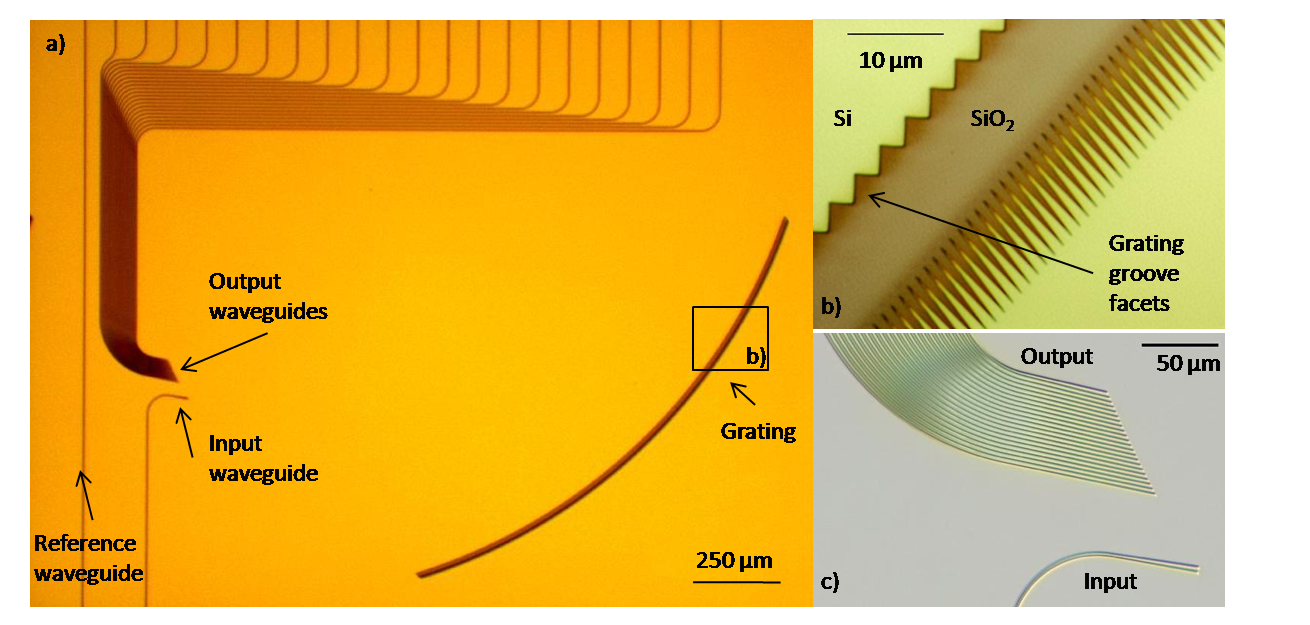
\includegraphics[width=1\textwidth]{./wdm}
\caption{Microscope photo of the WDM.}
\end{figure}
\subsection{Effective index dispersion} 
As previously discussed, the materials that the waveguide is made of and waveguide itself cause a dispersion of the effective refractive index of the mode. Figures \ref{fig:effective index dispersion} show the dispersion for TE mode slab waveguides with 200, 250 and 300 nm of thickness with material dispersion was used during calculation. Proper design needs to take into account this dispersion to position the output waveguides.
%
\begin{figure}[H]
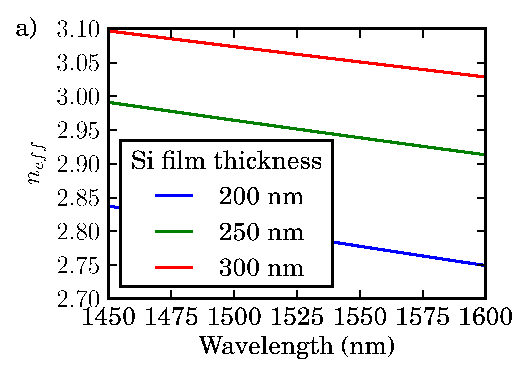
\includegraphics{graphs/slabDispersion}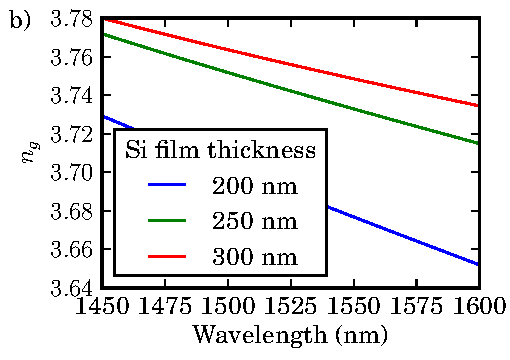
\includegraphics{graphs/slabGroupDispersion}
\caption{Effective index (a) and group index (b) dispersion for a Si slab waveguide surrounded by Silica for different slab thicknesses.}
\label{fig:effective index dispersion}
\end{figure}

\subsection{Fabrication}
\label{section:fabrication 1}
The fabrication was done in the \fnurl{Cornell Nanoscale Facility (CNF)}{http://www.cnf.cornell.edu}. A research micro-fabrication laboratory, funded in part by the National Science Foundation (NSF) and by its users. The research facility counts with state of the art electron beam lithography writer.

We fabricated the device using CMOS compatible procedures. First, we start with an SOI wafer with 250 nm silicon and 3 \textgreek{m}m buried oxide. An 80 nm layer of \ce{SiO2} was deposited using plasma enhanced chemical vapor deposition (PECVD) to be used as a hard mask. A 200 nm layer of PMMA was spun and then the grating and the waveguides were defined using e-beam lithography. The pattern was transferred from PMMA the to the oxide layer using \ce{CHF3}/\ce{O2} reactive ion etch. The silicon layer was etched using \ce{Cl2} inductively coupled plasma and then 2.3 \textgreek{m}m of \ce{SiO2} was deposited using PECVD to clad the device. The wafer was diced and polished for optical testing.
\begin{figure}[H]
\centering\input{fab.pdf_tex}
\caption{Fabrication process.}
\label{fig:fabrication}
\end{figure}

\subsection{Testing setup}
Testing was done by inserting a monochromatic tunable laser light in the device and measure the light power at each of the spectrometer output as the laser sweeps the wavelength.

The laser used was an external cavity laser (Tunics Reference) that has a line width of X pm. Light was guided in  fiber optic passed through a polarization controller and coupled in the chip waveguide using a lensed fiber, as shown in figures \ref{fig:setup photograph} and \ref{fig:setup schematics}. Light at the output waveguide is focused using a focusing lens pass through a polarizer, an iris and is detected. The iris was placed to block the light of channels neighboring the one is being measured. The lens, polarizer, iris and detector or mounted over a translation stage, figure \ref{fig:setup schematics}. The channel to be measured can be selected by translating the detection arrangement.
%
\begin{figure}[h]
\center{\input{setup.pdf_tex}}\caption{Experimental setup used to test the on chip spectrometer.}
\label{fig:setup photograph}
\end{figure}
%
\begin{figure}[h]
\center{\input{setup1.pdf_tex}}\caption{Schematics of the setup used to test the on chip spectrometer.}
\label{fig:setup schematics}
\end{figure}

\subsection{Results}
The measured performance of our \gls{WDM} showed -10 dB crosstalk and 1 nm channel spacing across 21 channels. As shown in figure \ref{fig:spectrum 1}, a relatively flat transmission spectrum was obtained. An insertion loss of -10 dB was estimated by comparing to the transmission through the reference waveguide. This can be attributed to Fresnel reflection between the Si-SiO2 interfaces at the grating groove facet and can be reduced by coating the grating facets with a reflective metal.
\begin{figure}[h]
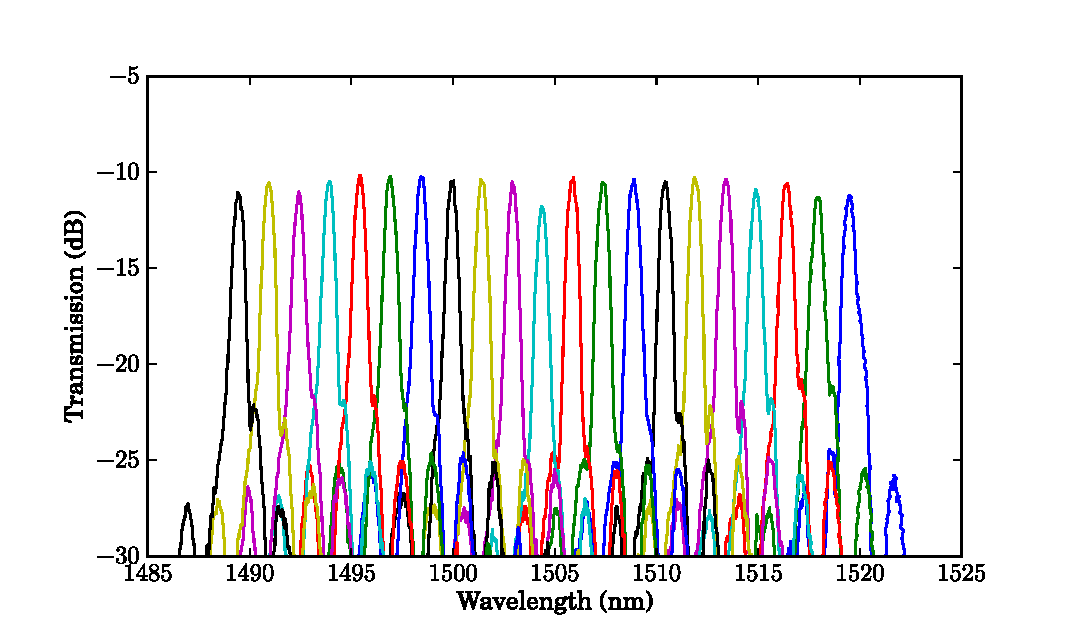
\includegraphics{graphs/gen5}
\caption{Transmission spectra of 21 channels of Rowland planar diffraction grating spectrometer.}
\label{fig:spectrum 1}
\end{figure}

\subsection{Conclusion}
In conclusion, we demonstrate a one point stigmatic Rowland grating \gls{WDM} with 21 channels, 1 nm channel spacing and better than -10 dB crosstalk. Since the free spectral range is greater the 100 nm, by adding additional output waveguides it is possible to construct a \gls{WDM} that covers whole C-band.%

\chapter{Ring Enhanced Spectrometer}
\epigraph{All for one, and one for all.}
{Alexandre Dumas}
How can we use resonators to make spectrometer? An array of resonators can be used. But fabrication limits prevent its use without requiring individually tuning each resonator. Grating spectrometers uses a lot of space. Is there a middle way. Yes! we can use small free spectral range resonators and a grating spectrometer. The device described in this chapter was published on optics express and presented on the Conference of Lasers and Electro-Optics 2010 (CLEO) as an invited paper and received an honorable mention in the Maiman Student Paper Competition in the same conference.

\section{Device theory}
\begin{figure}[h]
	\begin{minipage}[t]{0.49\columnwidth}%/Users/bernardo/data/2009-10-04/graph.py 
	\input{resonator-enhanced-sep.pdf_tex}
	\caption{Block elements for the resonator and spectrometer.}
	\label{fig:resonator spectrometer blocks}
	\end{minipage}\hfill%
	\begin{minipage}[t]{0.49\columnwidth}%
	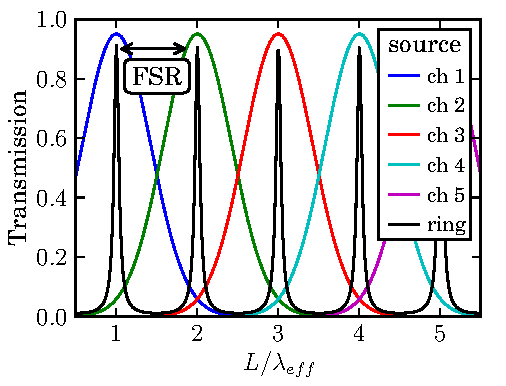
\includegraphics{ring-enhaced-sep}
	\caption{Transmission spectrum for the resonator and spectrometer on the left.}
	\label{fig:spectrum resonator spectrometer}
	\end{minipage}
\end{figure}
The principle of operation consists of using a resonator to pre-filter the light to be analyzed by a diffraction grating spectrometer. Initially we need a resonator and a spectrometer, figure \ref{fig:resonator spectrometer blocks}, with transmission spectrum such that the resonance peaks and the channels peaks coincide, figure \ref{fig:spectrum resonator spectrometer}. For this to happen, the resonator FSR and the spectrometer channels spacing needs to be equal, and the transmission peak of a spectrometer channel and a resonance peak needs to match.
\begin{figure}[h]
	\begin{minipage}[t]{0.49\columnwidth}%/Users/bernardo/data/2009-10-04/graph.py 
	\input{resonator-enhanced-tog.pdf_tex}
	\caption{Output of a resonator filter connected to the input of a spectrometer.}
	\label{fig:resonator connected spectrometer blocks}
	\end{minipage}\hfill
	\begin{minipage}[t]{0.49\columnwidth}%
	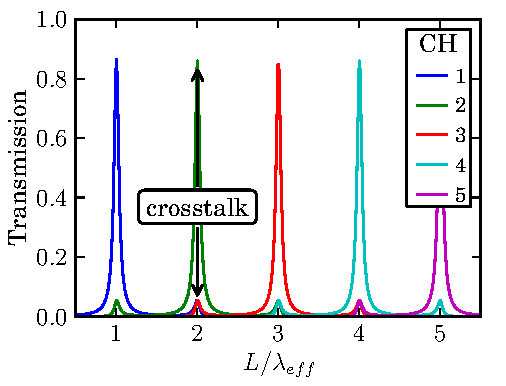
\includegraphics{ring-enhaced-tog}
	\caption{Transmission spectrum for the resonator connected to a spectrometer as depicted on the left. Small peaks are the overlap of the resonance neighboring the of a resonance t that match a channel peak and that channel residual transmission at that wavelength.}
	\label{fig:spectrum resonator connected spectrometer}
	\end{minipage}
\end{figure}
If we have this condition and we connect the resonator output to the spectrometer input, as in figure \ref{fig:resonator connected spectrometer blocks}, the transmission spectrum of the resulting device will be the overlap of the resonator and spectrometer transmission spectrum, figure \ref{fig:spectrum resonator connected spectrometer}.

The approach mix the high quality achievable by resonator with the multitude of channels offered by spectrometer.
%integration time independent of size

\section{Design}
Although the described mechanism can be realized with bulk components, as it has already been done\footcite{bajraszewski:2008p1743}, making these device using micro-fabrication techniques allow us to add more devices with little cost, which is of advantage when we increase channel density as we will see later.

For a PIC device, we used a ring cavity as the resonator and a diffraction grating spectrometer. As the DG spectrometer the same design as in section \ref{section:implementation} was used. A ring resonator with a drop port was designed to have 1 nm FSR in order to match the DG spectrometer channel spacing. Metal heaters are added above the silicon layer to align the resonator and spectrometer transmission combs using the thermo-optic effect in silicon. The diffraction grating spectrometer contains 25 channels. To match the ring resonator FSR to the DG spectrometer channel spacing we use an 83.5 \textgreek{m}m radius ring with waveguide cross-section of 450 x 250 nm. The FSR changes with wavelength according to $2\lambda/n_{g}L$, but considering a slight positive group velocity dispersion ($\partial n_{g}/\partial\lambda\approx3.6\times10^{-3}\text{nm}^{-1}$) this change is extremely small: the total change in FSR across the range of operation (25 nm) is approximately 1\% for light polarized in the plane of the device (TE polarization).

\section{Fabrication}

The fabrication of the dielectric part was carried the same way as the DG spectrometer, described in \ref{section:fabrication 1}. An alternation was done between layers before cladding the device with PECVD silicon oxide, which was to first cover the device conformally with 160 nm of \ce{SiO2} using a chemical vapor deposition at 1200\textdegree C. This was done because \ce{SiO2} deposited using PECVD was not completely filling the gap in the coupling to the ring waveguides. Here we only describe the additional steps to produce the ring heater.

In figure \ref{fig:fabrication heater}(a) we have the fabricated dielectric part as explained in figure \ref{fig:fabrication}. Over the cladding silica, we spin coat LOR5A (MicroChem) at 3000 RPM for 30 seconds and bake the result for 5 minutes in hot plate heated at 180\textdegree C. After letting the device cool down, SPR955CM (MicroChem) is spun coat at 4000 RPM for 30 seconds, and baked for 2 minutes in hot plate at 90\textdegree C,\ref{fig:fabrication heater}(b).

The ring heater pattern is then transferred from a previously patterned mask to the device using contact photolithography. The exposure time was 10 seconds with near-UV radiation (405-365 nm),\ref{fig:fabrication heater}(c). The mask was patterned using a pattern generator from the designed CAD file. Development was carried by imerging the sample in a solution of MIF300 (AZ Electronic Materials) for 60 seconds, and then rinsed for 20 seconds in de-ionized water,\ref{fig:fabrication heater}(d). 120 nm of NiCr was evaporated over the sample,\ref{fig:fabrication heater}(e). In the evaporator the sample was tied to a rotating disc, rotating at 200 RPM for the deposition to be angularly even. The resist together with the NiCr over it were striped leaving the device emerged in a solution of acetone overnight,\ref{fig:fabrication heater}(f). The device wafer was then diced and the pieces waveguide edges were polished.

%
\begin{figure}[h]
\input{fab2.pdf_tex}
\caption{Ring heater fabrication process.}
\label{fig:fabrication heater}
\end{figure}

\begin{figure}[h]
	\center{\input{chip2.pdf_tex}}
	\caption{}
\end{figure}


\section{Testing setup}
A similar setup used to test WDM was employed. In this setup electrical probe were added to drive current in the ring heater. Although it was not mentioned before, the base the chip rests over is a peltier heater-cooler with a thermocouple mounted on it to measure the temperature. Figure \ref{fig:setup2} shows a schematics of the setup.
\begin{figure}[h]
\center{\input{setup2.pdf_tex}}
\caption{Schematics of the setup used to test the ring enhanced spectrometer.}
\label{fig:setup2}
\end{figure}

To test the ring performance, light inserted in input waveguide is measured in the ring through port while the laser is scanned. Graph in figure \ref{fig:ring through spectrum} shows the through port transmission spectrum. Unfortunately the measured FSR was 0.97 nm, 30 pm lower than the designed. A zoom in the selected resonance shows, figure \ref{fig:resonance zoom}, shows that the FWHM is 50 pm, corresponding to a quality factor $Q=\lambda/\Delta\lambda=30000$. 
We measure the device transmission spectrum by coupling laser light from a tunable laser into the input waveguide using a lensed fiber and measuring the transmitted power as a function of wavelength. The input light is TE polarized and the output light is collected using a microscope objective and filtered for the TE polarization before detection. We achieve a channel \gls{FWHM} of 0.05 nm across 10 different channels of the composed ring and EDG spectrometer, which represents a decrease in the channel width by 10 times compared with the DG spectrometer alone. 
\begin{figure}[h]
\begin{minipage}[t]{0.49\columnwidth}%/Users/bernardo/data/2009-10-04/graph.py 
	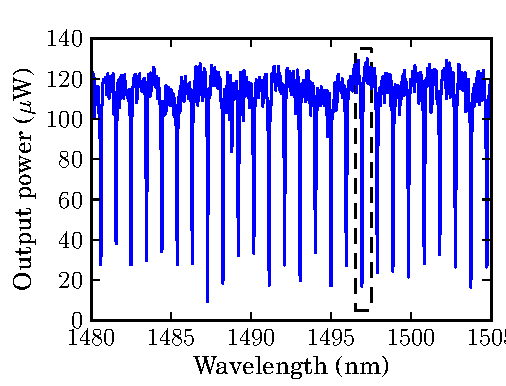
\includegraphics{ring-through}
	\caption{Output spectrum of the through port of the ring resonator.}
	\label{fig:ring through spectrum}
\end{minipage}\hfill{}%
\begin{minipage}[t]{0.49\columnwidth}%
	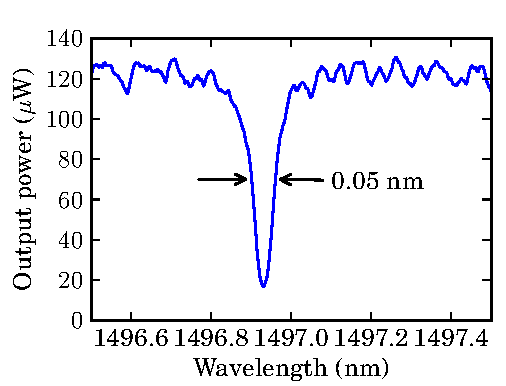
\includegraphics{ring-through-zoom}
	\caption{Zoom in the resonance marked on the left.}
	\label{fig:resonance zoom}
\end{minipage}
\end{figure}

Figure \ref{fig:RES spectrum} shows the device transmission. The transmission is normalized to the ring through port power level to eliminate coupling losses. The device insertion loss varies between -18 and -23 dB, where -10 dB is due to the Fresnel reflection of the diffraction grating and can be eliminated by coating it with a metal or using Bragg reflectors \footcite{Brouckaert:2008p108}. Other losses are attributed to stitching in the waveguide definition during e-beam lithography. A small mismatch between the resonator FSR (0.97 nm) and the DG spectrometer channel spacing (1 nm) cause a misalignment between the resonance and the DG spectrometer channel that builds up from one channel to the next in a Vernier effect. The outcome is a misalignment between the 11th spectrometer channel and the 11th ring resonance. Therefore only 10 of the 25 channels on the DG spectrometer are used. This issue can be eliminated by more detailed characterization of fabrication.
\begin{figure}[h] \noindent \begin{centering}
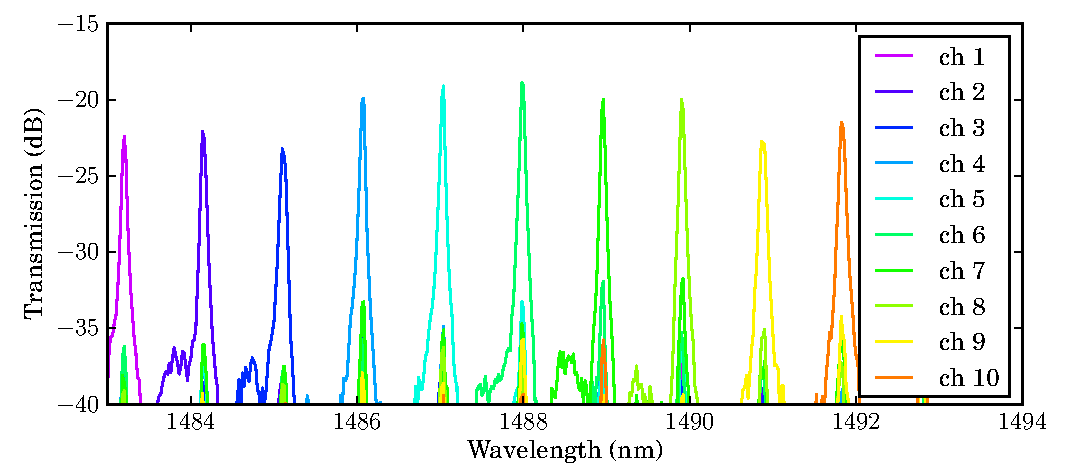
\includegraphics{graphs/low-density-ring-enhanced}
\par\end{centering}
\caption{Transmission spectrum for 10 channels of the ring enhanced spectrometer.\label{fig:RES spectrum}}
\end{figure} 


\section{Increasing channel density}

Channel width was greatly reduced due to the resonator. But the channel density, channels per unity of spectral range, is still equal to the DG spectrometer. Two ways can be readily suggested to increase the channel density. One denoted as space serialization and the other time serialization. 

The space serialization approach consists of using multiple combined ring-DG spectrometers, so that the input of a spectrometer is connected to the through port of the previous device, as shown in figure \ref{fig:RES tandem}. The peak wavelength of each spectrometer is shifted relative to the others. The number of devices needed in order to achieve the a spectral density where the channels are separated by $\Delta\lambda_{FWHM}$, is equal to the DG spectrometer channel width divided by $\Delta\lambda_{FWHM}$. In spite of the area increase, this approach is still more compact than using a traditional diffraction grating spectrometer since in this proposed approach the area increases linearly with resolution as opposed to quadratic in traditional DGs.
\begin{figure}[h]
	\begin{minipage}[t]{0.49\columnwidth}%/Users/bernardo/data/2009-10-04/graph.py 
		\input{tandem.pdf_tex}\caption{Multiple RES connected in tandem.\label{fig:RES tandem}}
	\end{minipage}\hfill{}%
	\begin{minipage}[t]{0.49\columnwidth}%
		\input{serial-time.pdf_tex}\caption{Single RES at difference temperature. Transmission spectrum shifts.\label{fig:RES temperature}}
	\end{minipage}
\end{figure}

In time serialization, figure \ref{fig:RES temperature}, only a single combined spectrometer is used and the output spectrum is measured several times. In each measurement the device transmission spectrum is shifted. Notice that this approach also requires active tuning of the ring and the EDG spectrometer. 

\section{Application of time serialization}
We applied the time serialization technique to our device. Thermo-optic effect was used to shift the spectrometer transmission spectrum. Since our FWHM was 50 pm and the channel spacing was 970 pm, we saw that an increment of channel density in 10 times could be done without introducing much crosstalk.

To achieve this, we would have to shift the ring resonances and EDG spectrometer channels by 97 pm. Watching a resonance of valley on the through port as we changed as the temperature, figure \ref{fig:resonance-tempshift} were changed we measured the rate of change of the resonance wavelength shift with temperature as being $79$ pm/K, figure \ref{fig:tempshift-fit}.
Resonance wavelength shift with ring heater driving power was also measured. It is checked whether the coefficient would change with the overall sample temperature. Although in principle this should happen, there was not an appreciable change in the range of temperature we driven the device.

Figure \ref{fig:transmission spectrum density} shows a density plot where each horizontal line corresponds to the transmission spectrum of each channel. Notice that the overlap of the residual transmission from the DG spectrometer with the neighboring resonances can be seen in the side diagonal lines, and their transmissions are at least 10 dB lower than the peak (main diagonal line).
%tempshift files in data/2009-10-06
\begin{figure}[H]
	\begin{minipage}[t]{0.49\columnwidth}
		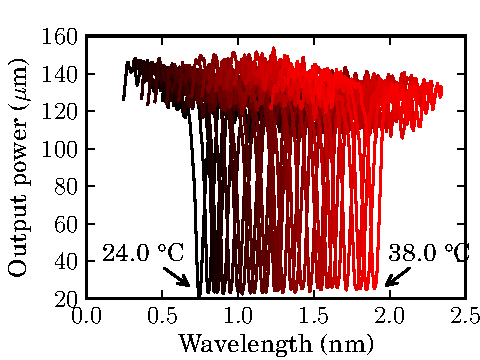
\includegraphics{resonance-tempshift}
		\caption{Through port output power as a temperature increase.}
		\label{fig:resonance-tempshift}
	\end{minipage}\hfill{}
	\begin{minipage}[t]{0.49\columnwidth}
		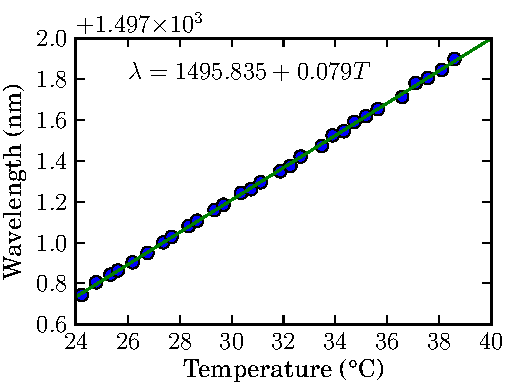
\includegraphics{tempshift-fit}
		\caption{Resonance wavelengths as temperature increases and fitted linear function.}
		\label{fig:tempshift-fit}
	\end{minipage}
\end{figure}
\begin{figure}[H]
	\begin{minipage}[t]{0.49\columnwidth}%/Users/bernardo/data/2009-10-04/graph.py 
		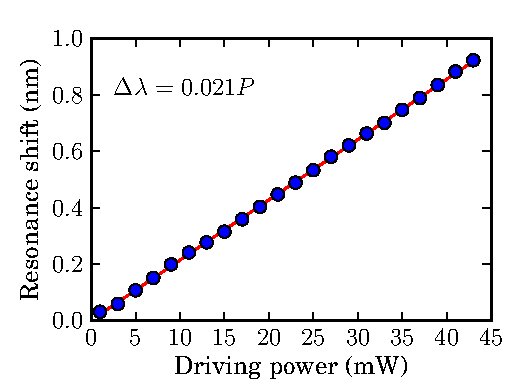
\includegraphics{ring-cal-fit}
		\caption{Resonance wavelength shift for the ring driven by different powers. Ring resistance is 2.2 k\textgreek{W}.}
		\label{fig:resonance shift resistance}
	\end{minipage}
\end{figure}

\section{Results}
\begin{figure}[H]
\noindent \centering{}
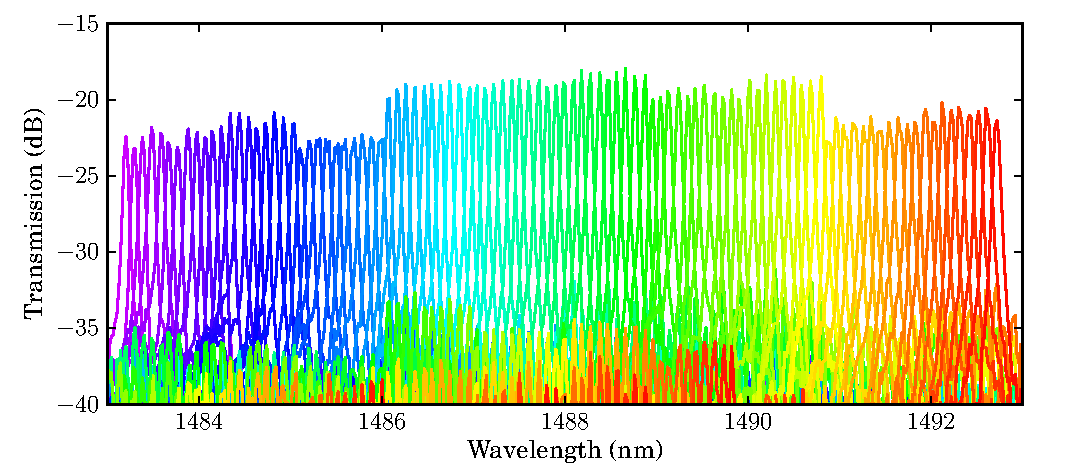
\includegraphics{graphs/hundred}
\caption{Transmission spectrum for a combined ring and diffraction spectrometer using a time serialization technique for reducing channel spacing.}
\label{fig:Transmission spectrum}
\end{figure}

Figure \ref{fig:Transmission spectrum} shows the transmission spectrum for the ring enhanced spectrometer for a set of 10 different temperature. We start with a configuration of chip temperature and ring heater driven power such that the DG comb and the ring resonances are aligned, the temperature of the chip is then raised in steps such that the transmission spectrum shifts by 97 pm.
%
\begin{figure}[h]
\noindent \begin{centering}
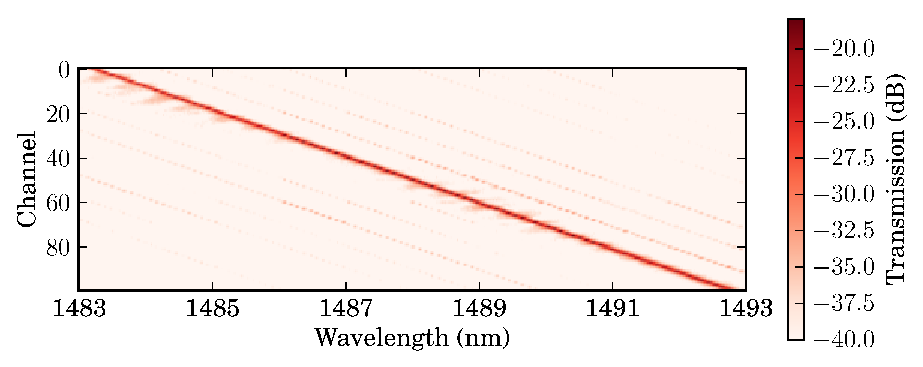
\includegraphics{graphs/hundred_density}
\par\end{centering}
\caption{Density plot of the transmission spectrum for a combined ring and diffraction spectrometer using a time serialization technique, where each horizontal line refers to a channel of the spectrometer.
\label{fig:transmission spectrum density}}
\end{figure}

\section{Device comparison}
\begin{table}[h]
\begin{centering}
\begin{threeparttable}[b]
\begin{tabular}{cccccc}
\hline 
Reference & Diagonal & Resolution & FSR & Crosstalk & Diagonal $\times$ Resolution\tabularnewline
      & (mm)   & (nm)    & (nm) & (dB)   & 			  \tabularnewline
\hline
\hline 
Brouckaert\tnote{1} & 0.3   & 20     & 150 & -30    & 6              \tabularnewline
Cheben\tnote{2}   & 11    & 0.2    & 10  & -10    & 2.2             \tabularnewline
Horst\tnote{3}   & 0.3   & 3.2    & 75  & -19    & 0.9             \tabularnewline
Current work\tnote{4}    & 1.4   & 0.1    & 115 & -8    & 0.14            \tabularnewline
\hline
\end{tabular}\caption{Comparison of integrated spectrometer features.\label{table:device comparison}}
\par
\begin{tablenotes}
\small
\item [1] \cite{Brouckaert:2007p82} \newline 
\item [2] \cite{Cheben:2007p133}\newline 
\item [3] \cite{Horst:2009p1764} \newline 
\item [4] \cite{Kyotoku:2010p786} 
\end{tablenotes}
\end{threeparttable}
\end{centering}
\end{table}

\section{About the DG spectrometer channels spacing and resonator FSR mismatch}
As mentioned, the mismatch between the DG spectrometer channel spacing and the resonator FSR caused a unalignment of the corresponding peaks that limited the useful set of spectrometer channels. It is interesting, therefore, to investigate how this interfere in production of RES.

The best alignment of the DG spectrometer channels and the resonance comb is achieved when the middle channel peak is matched with a resonance. In this configuration, the peak wavelength mismatch of the channel and resonance is going to be
\begin{equation}
\Delta\lambda_{\text{mismatch}}=\left(\Delta\lambda_{\text{CS}}-\Delta\lambda_{\text{FSR}}\right)\frac{N}{2},
\label{eq:missmatch}
\end{equation}
where $\Delta\lambda_{\text{CS}}$ is the DG spectrometer channel spacing, $\Delta\lambda_{\text{FSR}}$ is the resonator free spectral range, and $N$ is the number of spectrometer channels. Ideally we want a zero mismatch, but assuming that mismatch smaller than $\tau$ can be tolerated, we conclude that the tolerable relative channel spacing and resonator FSR error $\tau_{\text{error}}$ must be
\begin{equation}
\tau_{\text{error}}=\frac{\Delta\lambda_{\text{CS}}-\Delta\lambda_{\text{FSR}}}{\Delta\lambda_{\text{FSR}}}\le\frac{2\tau}{N\Delta\lambda_{\text{FSR}}}.
\label{eq:tolerable error}
\end{equation}
Supposing a tolerance equal half of the DG spectrometer channel FWHM for device with 100 channels and 1 nm channel spacing, a tolerable error of 1\% between the channel spacing and resonator FSR is reached.
To evaluate this result it is necessary to understand to what precision can we fabricate a device with determined FSR or channel spacing.

%\section{Effect of transmission spectrum lineshape}
%
%The effect that the transmission lineshape causes on the output spectrum is that the final measured spectrum is the convolution of the real spectrum with the channel transmission spectrum. The basic consequence is the limitation of the spectrometer resolution. For systems where the desired data is the Fourier transform of the output, such as optical coherence tomography and ultra fast oscilloscope, the transmission spectrum lineshape will cause a roll of as the frequency increases in the Fourier transform graph. This is due to the \fnurl{convolution theorem}{http://en.wikipedia.org/wiki/Convolution_theorem} that states that the Fourier transform of a convolution is the pointwise
%product of Fourier transforms of the convoluted functions.
%
%\footcite{Shi:2003p121}


\section{Conclusion}
Resonator enhanced spectrometer can improve device resolution. The fabrication using micro-fabrication techniques allow us to cheaply make several devices necessary for space serialization. never the less, studies must made in order to reliably manufacture devices where the resonance and spectrometer transmission comb are aligned through out a wide range of wavelength.


%%%%%%%%%%%%%%

swept source

integrate detectors
heaters on spectrometer
visible with silicon nitride

phase array for transversal scan


\printbibliography
\addcontentsline{toc}{chapter}{Bibliography}
%%%%%%%%%%%%%%%%%%%%%%%%%%%%%%%%%%%%%%%%%%%%%%%%%%%%%%%%%%%%%%%%%%%%%%%%%%%%%%%%%%%%%%%%%%%%%%%%
\appendix
%%\part{Appendix}
%\begin{table}
%\begin{tabular}{>{\centering}m{0.3\textwidth}c>{\centering}p{0.1\textwidth}>{\centering}p{0.4\textwidth}}
%\hline 
% & $f\left(x\right)$ & $F\left(x\right)=\int_{-\infty}^{\infty}f\left(x\right)e^{-2\pi ix\xi}dx$ & \medskip Remarks\medskip \tabularnewline
%\hline
%\hline 
%Rectangular $\leftrightarrow$ Sinc & $\text{rect}\left(ax\right)$ & ${\displaystyle \frac{1}{|a|}\cdot\text{sinc}\left(\frac{\xi}{a}\right)}$ & $\text{sinc}\left(x\right)=\frac{\sin\left(\pi x\right)}{\left(\pi x\right)}$\tabularnewline
%Gaussian $\leftrightarrow$ Gaussian & ${\displaystyle e^{-\alpha x^{2}}}$ & ${\displaystyle \sqrt{\frac{\pi}{\alpha}}\cdot e^{-\frac{(\pi\xi)^{2}}{\alpha}}}$ & Gaussian function is its own Fourier transform. $a>0$\tabularnewline
%Exponential $\leftrightarrow$ Lorentzian & $e^{-a|x|}$ & ${\displaystyle \frac{2a}{a^{2}+4\pi^{2}\xi^{2}}}$ & $a>0$\tabularnewline
%Exponential pulse $\leftrightarrow$ & ${\displaystyle e^{-ax}H(x)}$ & ${\displaystyle \frac{1}{a+2\pi i\xi}}$ & $H\left(x\right)$ is the Heaviside unit step function. $\Re\left(a\right)>0$\tabularnewline
%\hline
%\end{tabular}
%
%\caption{}
%
%\end{table}
%\chapter{}
%
%For numerical computations some further simplifications can be done to the model described on section \ref{section:Rayleigh-Huygens-model}.
%
%%
%\begin{figure}[h]
%\noindent \centering{}\input{KHapendix1.pdf_tex}\caption{}
%
%\end{figure}
%\begin{equation}
%\begin{cases}
%P_{x}=I_{x}-y\sin\iota\\
%P_{y}=I_{y}+y\cos\iota\end{cases}\end{equation}
%\begin{equation}
%\begin{cases}
%P'_{x}=I_{x}+r\cos\left(\iota+\alpha\right)\\
%P'{}_{y}=I_{y}+r\sin\left(\iota+\alpha\right)\end{cases}\end{equation}
%\begin{equation}
%\begin{cases}
%P'_{x}=P_{x}+r'\cos\left(\iota+\alpha'\right)\\
%P'{}_{y}=P_{y}+r'\sin\left(\iota+\alpha'\right)\end{cases}\end{equation}
%\begin{equation}
%\begin{cases}
%P'_{x}=I_{x}-y\sin\iota+r'\cos\alpha'\\
%P'{}_{y}=I_{y}+y\cos\iota+r'\sin\alpha'\end{cases}\end{equation}
%\begin{equation}
%r_{1}=\left|P'-I\right|\end{equation}
%\begin{equation}
%r'_{1}=\left|P'-P\right|\end{equation}
%\begin{equation}
%r'^{2}=\left(P'_{y}-P_{y}\right)^{2}+P'_{x}\end{equation}
%\begin{equation}
%r'=\sqrt{\left(r\sin\alpha-P_{y}\right)^{2}+r\cos^{2}\alpha}\end{equation}
%\begin{equation}
%r'=\sqrt{r^{2}-2P_{y}r\sin\alpha+P_{y}^{2}}\end{equation}
%\begin{equation}
%r'=r\sqrt{1-2\frac{P_{y}}{r}\sin\alpha+\left(\frac{P_{y}}{r}\right)^{2}}\end{equation}
%\begin{equation}
%r'=r\left[1-\frac{P_{y}}{r}\sin\alpha+O\left(2\right)\right]\end{equation}
%for\begin{equation}
%\cos\alpha'=\sqrt{1-\sin^{2}\alpha'}=\sqrt{1-\left(\frac{P'_{y}-P_{y}}{r'}\right)^{2}}=\sqrt{1-\left[\frac{r\left(\sin\alpha-\frac{P_{y}}{r}\right)}{r\left(1-\frac{P_{y}}{r}\sin\alpha\right)}\right]^{2}}\approx\cos\alpha+\frac{P_{y}}{r}\sin\alpha\cos\alpha\end{equation}
%\begin{equation}
%\frac{1}{\sqrt{r'}}=\frac{1}{\sqrt{r}}\frac{1}{1-\frac{P_{y}}{r}\sin\alpha+O\left(2\right)}\approx\frac{1}{\sqrt{r}}\left(1+\frac{P_{y}}{2r}\sin\alpha\right)\end{equation}
%Putting all together:\begin{equation}
%E_{inc}=\frac{1}{2}\sqrt{\frac{n_{eff}}{\lambda}}\int E_{wg}\left(y\right)\frac{e^{-ikr'}}{\sqrt{r'}}\left(1+\cos\alpha'\right)dP_{y}\end{equation}
%dsd $E_{wg}\left(y\right)=E\exp\left[-4\ln2\left(\frac{P_{y}}{w}\right)^{2}\right]$\begin{equation}
%E_{inc}=\frac{1}{2}\sqrt{\frac{n_{eff}}{\lambda}}\int E_{wg}\left(y\right)\frac{e^{-ikr+ikP_{y}\sin\alpha}}{\sqrt{r}}\left(1+\frac{P_{y}}{2r}\sin\alpha\right)\left(1+\cos\alpha+\frac{P_{y}}{r}\sin\alpha\cos\alpha\right)dP_{y}\end{equation}
%\begin{equation}
%E_{inc}=\frac{1}{2}\sqrt{\frac{n_{eff}}{\lambda}}\int E\exp\left[-4\ln2\left(\frac{P_{y}}{w}\right)^{2}\right]\frac{e^{-ikr+ikP_{y}\sin\alpha}}{\sqrt{r}}\left(1+\frac{P_{y}}{2r}\sin\alpha\right)\left(1+\cos\alpha+\frac{P_{y}}{r}\sin\alpha\cos\alpha\right)dP_{y}\end{equation}
%\begin{equation}
%E_{inc}=\frac{1}{2}\sqrt{\frac{n_{eff}}{\lambda}}\frac{E}{\sqrt{r}}\int\exp\left[-4\ln2\left(\frac{P_{y}}{w}\right)^{2}\right]e^{-ikr}e^{-ikP_{y}\sin\alpha}\left(1+\cos\alpha+\frac{P_{y}}{r}\left(\frac{1}{2}+\frac{3}{2}\sin\alpha\cos\alpha\right)+\frac{1}{2}\left(\frac{P_{y}}{r}\right)^{2}\sin^{2}\alpha\cos\alpha\right)dP_{y}\end{equation}
%\begin{equation}
%E_{inc}=\frac{1}{2}\sqrt{\frac{n_{eff}}{\lambda}}\frac{E}{\sqrt{r}}e^{-ikr}\left\{ \left(1+\cos\alpha\right)\int\exp\left[-4\ln2\left(\frac{P_{y}}{w}\right)^{2}\right]e^{-ikP_{y}\sin\alpha}dP_{y}+\frac{1}{r}\left(\frac{1}{2}+\frac{3}{2}\sin\alpha\cos\alpha\right)\int\exp\left[-4\ln2\left(\frac{P_{y}}{w}\right)^{2}\right]e^{-ikP_{y}\sin\alpha}P_{y}dP_{y}\right\} \end{equation}
\chapter{Huygens-Fresnel Diffraction}
\section{Numerical calculation}

On computing Helmholts and Kirchhoff integral theorem \ref{eq:integral theorem} numerically, a few optimization can be made. The following optimization is particulary usefull when the calculation needs to be taken over many elements. To make it more clear, consider the arrangement in figure \ref{fig:many diff el arr}. 
\begin{figure}[h]
\centering
\input{KHgeneral.pdf_tex}
\caption{}
\label{fig:many diff el arr}
\end{figure}
We have a light source at point $S$ and two obstacles that have apertures $\mathbb{Q}$ and $\mathbb{P}$, and we want to evaluate the electric field at $T$. Using the integral theorem, this would be a three step operation. First we would compute the field at $\mathbb{Q}$ from $S$, then compute field at $\mathbb{P}$ from field at $\mathbb{Q}$, to then finally calculate the field at $T$ from the field at $\mathbb{P}$. From the integral theorem we see that at each point $P$ we need to compute the field $U(P)$ and derivative of the field in the direction of normal $\hat{m}$ of apperture defining plane $\mathbb{P}$, $\frac{\partial U\left(P\right)}{\partial m}$. By analytacally carrying the derivative of $U$ in respect of $\hat{m}$, numerical derivative is avoided which would introduce \fnurl{round-off error}{http://en.wikipedia.org/wiki/Rounding_error} and processing cost. The resulting pair of equations will then be.
\begin{equation}
U\left(P\right)=\int_{\mathbb{Q}}\frac{e^{\text{i}kr}}{\sqrt{kr}}\left[\frac{ikU\left(Q\right)}{2}\cos\left(r,n\right)-\frac{\partial U\left(Q\right)}{\partial n}\right]dS\end{equation}
\begin{equation}
\frac{\partial U\left(P\right)}{\partial m}=\frac{ik}{2}\int_{\mathbb{Q}}\frac{e^{\text{i}kr}}{\sqrt{kr}}\left[U\left(Q\right)\frac{ik}{2}\cos\left(r,n\right)-\frac{\partial U\left(Q\right)}{\partial n}\right]\cos\left(r,m\right)dS\end{equation}
We, then, can use the above set of equations to iteractively compute the electric field at points $Q$, $P$ and $T$.

\section{Small aperture approximation}
If the aperture $\mathbb{Q}$ is much smaller than $r$, then we can consider that $\cos\left(r,m\right)$ does not vary a lot in the integral, therefore we can pull it outside the integral, which convert the integral to $U\left(P\right)$. We therefore can simplify the equations to
\begin{equation}
\begin{cases}
U\left(P\right)=\int_{\mathbb{Q}}\frac{e^{\text{i}kr}}{\sqrt{kr}}\left[\frac{ikU\left(Q\right)}{2}\cos\left(r,n\right)-\frac{\partial U\left(Q\right)}{\partial n}\right]dS\\
\frac{\partial U\left(P\right)}{\partial m}=\frac{ik}{2}\cos\left(r,m\right)U\left(P\right)\end{cases}\end{equation}
\begin{equation}
\frac{\partial U\left(P\right)}{\partial m}=\frac{ik}{2}\cos\left(r,m\right)\int_{\mathbb{Q}}\frac{e^{\text{i}kr}}{\sqrt{kr}}\left[U\left(Q\right)\frac{ik}{2}\cos\left(r,n\right)-\frac{\partial U\left(Q\right)}{\partial n}\right]dS=\frac{ik}{2}\cos\left(r,m\right)U\left(P\right)\end{equation}

\section{Numerical program validation}
To validate the program, we simulated a geometry that could also be solved analytically. Figure shows the chosen geometry. It consists of a circular screen with radius $R$, and a source field concentric with the screen consisting of a uniform field $E$ over a line segment with length $W$. Analytically the first approximation off equation, to the chosen geometry will be equal to
\begin{equation}
E_{\text{circle}}=\sqrt{\frac{\pi }{2}} W E e^{-i k R} \sqrt{\frac{k}{R}} (\cos (\alpha )+1) \text{sinc}\left(\frac{k W \sin (\alpha )}{2 \pi }\right)
\end{equation}
where $k$ is the wavenumber. For $R=2\text{mm}$, $k=1.24\times10^5\text{cm}^-1$ and $W=3$\textgreek{m}m, the simulation (circle markers) and analytic function (continuous line) are plotted in figure X.
\begin{figure}[h]
\input{validation-geometry.pdf_tex}
\hfill
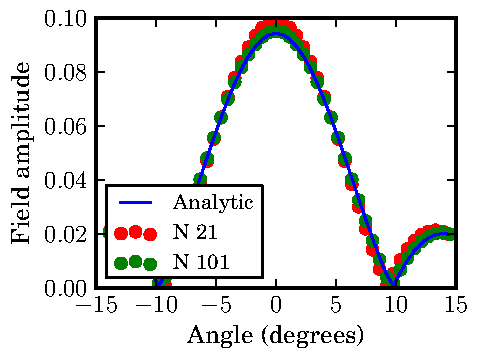
\includegraphics{compare-analytic.pdf}
\caption{(a) Schematic of the geometry used to validate simulation program against the analytic solution. (b) Electric field in the circle screen in (a) versus the angle $\alpha$.}
\label{fig:program validation}
\end{figure}
%\section*{Cosine does not vary much}
%
%We can enclose $\mathbb{Q}$ by a circle of radius $q$ centered
%at $Q_{C}$, we therefore can write any point of Q by $Q=Q_{C}+v$
%where $\left|v\right|<q$. And we define $\vec{r}'=P-Q_{C}$\begin{equation}
%\end{equation}
%\begin{equation}
%\cos\left(r,m\right)=\frac{\vec{r}\cdot\hat{m}}{r}=\frac{\left(P-Q\right)\cdot\hat{m}}{\left|P-Q\right|}\end{equation}
%\begin{equation}
%\cos\left(r,m\right)=\frac{\vec{r}\cdot\hat{m}}{r}=\frac{\left(P-Q_{C}-v\right)\cdot\hat{m}}{\left|P-Q_{C}-v\right|}=\frac{\vec{r}'\cdot\hat{m}-\vec{v}\cdot\hat{m}}{\left|\vec{r}'-\vec{v}\right|}=\frac{\vec{r'}\cdot\hat{m}}{\left|\vec{r}'-\vec{v}\right|}-\frac{\vec{v}\cdot\hat{m}}{\left|\vec{r}'-\vec{v}\right|}=\frac{r'\cos\left(r',m\right)}{\left|\vec{r'}-\vec{v}\right|}-\frac{v\cos\left(v,m\right)}{\left|\vec{r'}-\vec{v}\right|}\end{equation}
%\begin{equation}
%\left|\vec{r'}-\vec{v}\right|=\sqrt{r'^{2}+v^{2}+r'v\cos\left(r,v\right)}=r'\sqrt{1+\frac{v^{2}}{r'^{2}}+\frac{v}{r'}\cos\left(r,v\right)}\end{equation}
%\begin{equation}
%\cos\left(r,m\right)=\frac{\cos\left(r',m\right)}{\sqrt{1+\frac{v^{2}}{r'^{2}}+\frac{v}{r'}\cos\left(r,v\right)}}-\frac{v}{r'}\frac{\cos\left(v,m\right)}{\sqrt{1+\frac{v^{2}}{r'^{2}}+\frac{v}{r'}\cos\left(r,v\right)}}\end{equation}
%since $v<q\ll r'$, then at first approximation $\cos\left(r,m\right)=\cos\left(r',m\right)+O\left(\frac{q}{r'}\right)$
%


\chapter{Fourier transform}

\section{Relation}
\begin{equation}
\sum_{n=-\infty}^{\infty}f\left(n\right)e^{ikn}=\sum_{m=-\infty}^{\infty}\hat{f}\left(\frac{k}{2\pi}-m\right)
\label{eq:fourier series relation}
\end{equation}
Using Dirac delta integral
\[
\sum_{n=-\infty}^{\infty}f\left(n\right)e^{ikn}=\sum_{n=-\infty}^{\infty}\int_{-\infty}^{\infty}\delta\left(x-n\right)f\left(x\right)e^{ikx}dx,\]
which can be reordered to
\[
\sum_{n=-\infty}^{\infty}f\left(n\right)e^{ikn}=\int_{-\infty}^{\infty}f\left(x\right)\sum_{n=-\infty}^{\infty}\delta\left(x-n\right)e^{ikx}dx.\]
Using the relation $\sum_{n=-\infty}^{\infty}\delta\left(x-n\right)=\sum_{m=-\infty}^{\infty}e^{-2\pi mx}$
\[
\sum_{n=-\infty}^{\infty}f\left(n\right)e^{ikn}=\int_{-\infty}^{\infty}f\left(x\right)\sum_{m=-\infty}^{\infty}e^{-2\pi mx}e^{ikx}dx,\]
and reordering the sum\[
\sum_{n=-\infty}^{\infty}f\left(n\right)e^{ikn}=\sum_{m=-\infty}^{\infty}\int_{-\infty}^{\infty}f\left(x\right)e^{i2\pi\left(\frac{k}{2\pi}-m\right)x}dx.\]
Notice that the integral is Fourier transform then we get,\[
\sum_{n=-\infty}^{\infty}f\left(n\right)e^{ikn}=\sum_{m=-\infty}^{\infty}\hat{f}\left(\frac{k}{2\pi}-m\right)\]
Q.E.D.
\section{Common Fourier transforms}
\begin{table}[h]
\centering
\begin{tabular}{|>{\centering}m{0.1\textwidth}|>{\centering}m{0.25\textwidth}|>{\centering}m{0.25\textwidth}|>{\centering}m{0.30\textwidth}|}
\hline 
Function & 
Fourier transform unitary, ordinary frequency & 
Fourier transform unitary, angular frequency & 
Remarks
\tabularnewline%%%%%%%%%%%%%%%%%%%%%%%%%%%%%%%%%%%%
\hline
\hline 
$f\left(x\right)$ &
$\hat{f}(\xi)={ \int_{-\infty}^{\infty}f(x)e^{-2\pi ix\xi}\, dx}$ &
$\hat{f}(\omega)={ \frac{1}{\sqrt{2\pi}}\int_{-\infty}^{\infty}f(x)e^{-i\omega x}\, dx}$ &
\tabularnewline%%%%%%%%%%%%%%%%%%%%%%%%%%%%%%%%%%%%
\hline 
$\text{rect}\left(ax\right)$ &
$\frac{1}{\left|a\right|}\cdot\text{sinc}\left(\frac{\xi}{a}\right)$ &
$\frac{1}{\sqrt{2\pi a^{2}}}\cdot\text{sinc}\left(\frac{\omega}{2\pi a}\right)$ &
where $\text{sinc}\left(x\right)=\sin\left(\pi x\right)/\left(\pi x\right)$.
\tabularnewline%%%%%%%%%%%%%%%%%%%%%%%%%%%%%%%%%%%%
\hline 
$e^{-ax}S\left(x\right)$ &
$\frac{1}{a+2\pi i\xi}$ &
${ \frac{1}{\sqrt{2\pi}(a+i\omega)}}$ & 
The function $S\left(x\right)$ is the Heaviside unit step function
and $a>0$.
\tabularnewline%%%%%%%%%%%%%%%%%%%%%%%%%%%%%%%%%%%%
\hline 
$e^{-\alpha x^{2}}$ & 
${ \sqrt{\frac{\pi}{\alpha}}\cdot e^{-\frac{(\pi\xi)^{2}}{\alpha}}}$ & 
$\frac{1}{\sqrt{2\alpha}}\cdot e^{-\frac{\omega^{2}}{4\alpha}}$ & 
For this to be integrable we must have $\text{Re}\left(\textgreek{a}\right)>0$.\tabularnewline%%%%%%%%%%%%%%%%%%%%%%%%%%%%%%%%%%%%
\hline
\end{tabular}\caption{Fourier transform of function found in the text.\label{table:fourier transform}}

\end{table}
%\printbibliography
%\bibliographystyle{unsrt}
%\bibliography{abibliography}
\printglossaries
\end{document}
